\documentclass[twoside]{protokoll}
\usepackage{graphicx}
\usepackage{tabularx}
\usepackage{booktabs}
\usepackage{float} 
\praktikum{I}
\usepackage{subfig}
\usepackage{amsmath}

\versuchsgebiet{(Mechanik)}


\teilnehmer{Maximilian Carlos Menke, 434170}
\teilnehmer{Andrea Roth, 428396}
\gruppe{A3}

\begin{document}
 
\section{1M1 Messung der Erdbeschleunigung mit dem Pendel}
 
\begin{aufgabe}{Grundlagen}
  Knappe Beschreibung der theoretischen Grundlagen, Angabe der
  benötigten Formel(n), ohne Herleitung. Definition der verwendeten
  Formelzeichen.
\end{aufgabe}

\section{Grundlagen}

Das Pendel in diesem Versuch, welches aus einem Pendelkörper, einer Pendelstange und einer Aufhängung, bei welcher zwei Nadeln in die Nut eines Winkelaufnehmers gestellt werden, besteht kann als Physikalisches Pendel betrachtet werden.
Den Genauen Aufbau des Pendels können sie Skizze \ref{Pendel Aufbau} entnehmen.
Dabei wirkt auf das Pendel eine Kraft von $F_g = m_S \cdot g$, wobei $g$ die zu bestimmende Erdbeschleunigung ist und $m_S$ die Schwere Masse des Pendels.
Beim Schwingen, befindet sich das Pendel oftmals nicht in der Ruhelage, sondern ist um den Winkel $\varphi$ vom Gleichgewichtszustand Ausgelenkt.
Dann wirkt ein rückstellendes Drehmoment $ M = l \cdot F_r$ (mit $l$ als Länge von der Rotationsachse zum Schwerpunkt).
Da unser Pendel Träge ist, entsteht eine Schwingung: 
\begin{equation}
    J \cdot \ddot{\varphi} = -m \cdot g \cdot l^2 \cdot \sin(\varphi)
\end{equation}
Dabei verwenden wir im Folgenden die Kleinwinkel Näherung $\sin(\varphi) \approx \varphi$.
Diese gilt für Auslenkungen von weniger als $5$°. Damit lässt sich die Bewegungsgleichung vereinfachen:
\begin{equation}
    J \cdot \ddot{\varphi} \approx -m \cdot g \cdot l^2 \cdot \varphi
\end{equation}
Das Trägheitsmoment ist dabei wie folgt definiert:
\begin{equation}
    J =  m_T \cdot l^2
\end{equation}
Hierbei ist $m_T$ die Träge Masse des Pendels. Dies ist nach dem Einsteinnischen Äquivalenzprinzip aber gleich der schweren Masse, und somit $m_T = m$.
Aufgelöst nach $\ddot{\varphi}$ ergibt sich ( mit $\omega = 2 \pi f = \frac{2 \pi}{T}$) als Winkelgeschwindigkeit der Schwingung):
\begin{equation}
    \ddot{\varphi} \approx -\frac{g}{l} \cdot \varphi = - \omega^2 \cdot \varphi
\end{equation}
Aus dieser DGL lässt sich $\varphi(t)$ bestimmen, zu:
\begin{equation}
    \varphi(t) = \varphi_{max} \cdot \cos(\omega \cdot t)
\end{equation}
Daraus ergibt sich (mit $T$ als Dauer einer Schwingungsperiode):
\begin{equation}
    \omega^2 = \frac{m \cdot g \cdot l_s}{J}
\end{equation}
\begin{equation}
    \Rightarrow T = \frac{1}{g} 4 \cdot \pi^2 \cdot \frac{J}{m l_s}
    \label{periodendauer}
\end{equation}
Dabei kann man $\omega$ als Quotient von rückstellendes Drehmoment und Trägheitsmoment beschreiben.
Hier sind alle Größen mit einem einem $_{G}$ versehen sind dem Pendel mit Stange und Gewicht zugehörig. Die mit einem $_{st}$ versehenen Größen gehören nur zur Stange.
\begin{equation}
    \omega_{st}^2 = \frac{M_{st}}{J_{st}}
\end{equation}
\begin{equation}
    \omega_{G}^2 = \frac{M_G}{J_G} = \frac{M_{st} + M_P}{J_{st} + J_P}
\end{equation}
Hierbei sind $M_P$ und $J_P$ das Trägheitsmoment und das rückstellende Drehmoment welche auf das zusätzliche angebrachte Gewicht wirken.
Wenn man die Position des Gewichtes so einstellt, dass die Schwingung der Stange die gleiche Periodendauer hat wie die Schwingung der Stange mit Gewichtes, dann gilt:
\begin{equation}
    \omega_{st}^2 = \omega_{G}^2
\end{equation}
\begin{equation}
    \omega^2 = \omega_p^2 \frac{1 + \frac{M_{st}}{M_P}}{1+\frac{J_{st}}{J_P}} = \omega_{st}^2 \frac{1 + \frac{M_P}{M_{st}}}{1+\frac{J_P}{J_{st}}}
\end{equation}
\begin{equation}
    \Rightarrow \frac{M_P}{M_{st}} = \frac{J_P}{J_{st}}
\end{equation}
\begin{equation}
    \Rightarrow \frac{M_P}{M_{st}} = \frac{J_P}{J_{st}}
\end{equation}
\begin{equation}
    \omega^2 = \frac{M_{st}}{J_{st}} = \frac{M_P}{J_P}
\end{equation}
Folgich da alle Frequenz gleich sind, kann man $\frac{M_G}{J_G} = \omega_{st}^2 = \frac{M_{st}}{J_{st}}$ ersetzen.
Das bedeutet das wir das Pendel mit Gewicht so behandeln können, als würde nur der Pendelkörper schwingen. 
Es macht also kein Unterschied, ob wir die Stange weg lassen oder den Pendelkörper in unseren Berechnungen. \\
Nun muss noch das Trägheitsmoment des Gewichtes bestimmt werden.
Für das Trägheitsmoment des Gewichtes wenn dieses in der Rotationsachse liegen würde, kann das Trägheitsmoment eines Zylinders verwendet werden.
Mit dem Satz von Steiner kann noch das zusätzliche Trägheitsmoment bestimmt werden, welches durch die Verschiebung der Rotationsachse entsteht. (2. Summand)
\begin{equation}
    J_G = \frac{1}{2} m_G \cdot r_G^2 + m_G \cdot l_G^2
\end{equation}
Hier ist $r_G$ der Radius des Gewichtes und $l_G$ der Abstand vom Gewicht zur Rotationsachse.
Wenn man das Drehmoment und das Trägheitsmoment jetzt explizit ausdrückt, dann erhält man:
 
Wie mit Gln. \ref{periodendauer} zu sehen ist, kann die Periodendauer verkleinert werden, wenn $J_G$ verkleinert wird.
Dies kann man erreichen, indem $l_G$ kleiner wird. So kann man das Pendel mit Gewicht auf die gleiche Periodendauer wie das Pendel ohne Gewicht bringen. \\

Es ergibt sich:
 
\begin{equation}
    \omega^2 = \frac{m_G \cdot g \cdot l_G}{\frac{1}{2} m_G \cdot r_G^2 + m_G \cdot l_G^2}
\end{equation}
Nach $g$ Aufgelöst ergibt sich:
\begin{equation}
    g = \omega^2 \cdot l_G \left( 1 + \frac{r_G^2}{2 \cdot l_G^2} \right)
    \label{eq:pendel_g}
\end{equation}


Die Auslenkung des Winkels messen wir dabei mit der Hall-Sonde.
Das Magnetfeld kann dabei so orientiert werden, dass es vertikal steht.
Die Hall-Spannung wird dabei von der Hall-Konstante und  der Dicke des stromdurchflossenen Plättchens beeinflusst.
Hinzu kommt noch das Kreuzprodukt von Magnetfeld und Stromstärke. Da sowohl das Magnetfeld als auch der Stromfluss konstant sind, hängt das Kreuzprodukt nur vom Sinus des Winkels der beiden ab.
Da wir nur kleine Winkel betrachten, kann man in guter Näherung annehmen, das $\sin(\varphi) \approx \varphi$ ist.
Folglich ist die Hall-Spannung nur proportional zur Auslenkung des Winkels, da alle anderen Größen konstant sind.
Deshalb können wir mit der Hall-Sonde unsere Schwingung aufzeichnen.



\begin{aufgabe}{Versuchsaufbau und Versuchsdurchführung}
  Beschreibung des Versuchsaufbaus einschließlich beschrifteter Skizze
  oder Foto. Beschreibung der Versuchsdurchführung: Handgriffe an der
  Apparatur, verwendete Messwerterfassungseinstellungen, Messbereiche,
  Triggerbedingungen, etc.
\end{aufgabe}

\section{Aufbau und Durchführung}
Kurz zusammengefasst besteht der Versuchsaufbau aus einem Stabilen dreieckigen Stativ, an welchem ein Winkelaufnehmer befestigt wird.
An diesen Winkelaufnehmer Wird ein Pendel gehangen, welches aus einem U-Profil, mit zwei Metallnadeln als Aufhängung, einer flachen Pendelstange, und einem Pendelkörper besteht.\\
\subsection{Aufbau}
\begin{figure}[H]
    \centering
    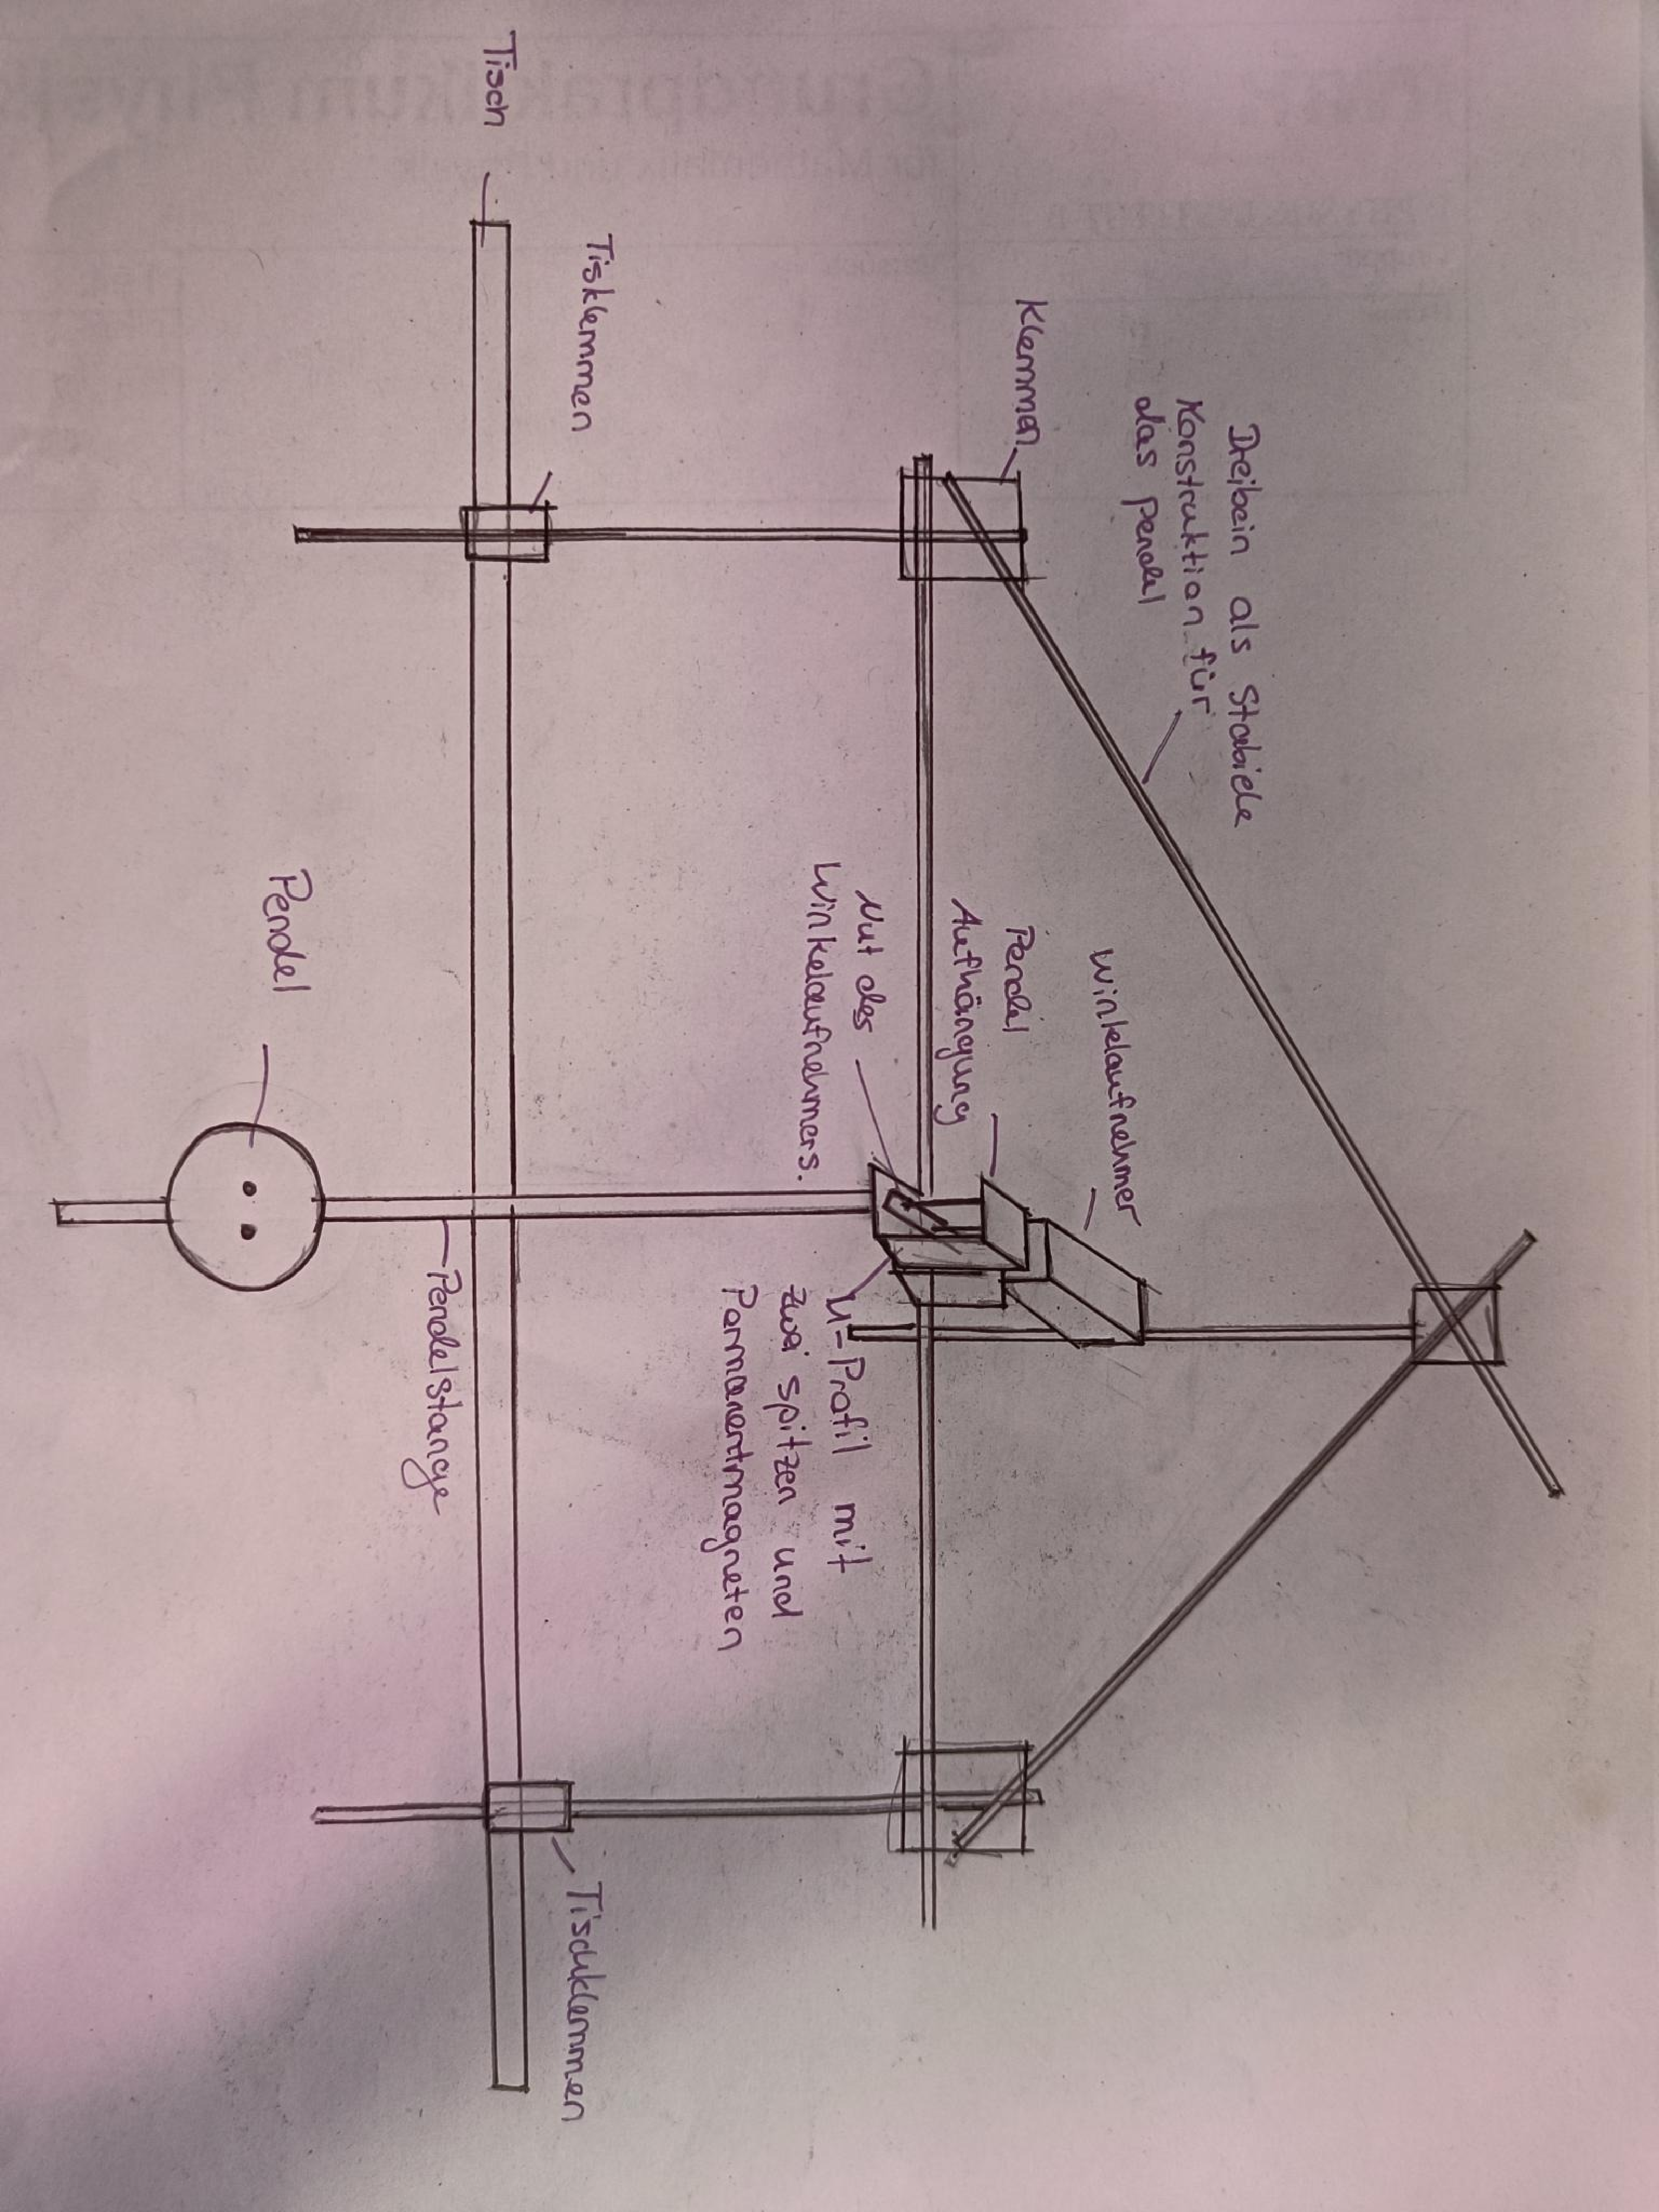
\includegraphics[width=0.9\textwidth]{Bilder/Kompletter-Aufbau.pdf}
    \caption{Nahaufnahme von der Nut mit Nadel}
\end{figure}

Der Oberen Skizze kann der Gesamtaufbau entnommen werden. 
Zunächst werden zwei Tischklemmen mit je einer Stativ Stange am vorderen Tisch befestigt.
Die dritte Stativ Stange wird auf der anderen Seite des Tisches in der bereits angebrachten Halterung befestigt. 
Mit Kreuzmuffen (in Skizze mit Klemme beschriftet) werden nun die langen Metallstangen verwendet um diese 3 Stativ Stangen zu verbinden, und so ein Dreieck zu bilden.
Es sollte darauf geachtet, werden, das die Stangen gut in den Kreuzmuffen liegen. 
Bei der vorderen Stange an welcher später das Pendel auf gehangen wird, muss darauf geachtet werden, dass diese horizontal ist.
Dies kann mithilfe der Wasserwaage überprüft werden.\\

Wenn diese Konstruktion stabil ist, kann vorne an der Stange der Winkelaufnehmer befestigt werden. 
Dieser besteht aus einer Stange in welcher 2 Nut sind mit einer Hall-Sonde. 
Dies wird an das CASSY angeschlossen.
Wir haben beide Winkelaufnehmer befestigt, um zu überprüfen welchen wir besser Nullen können, und damit wir später ein Pendel mit und eins ohne Pendelkörper bei der Synchronisation vergleichen können.
Bei den Winkelaufnehmern muss darauf geachtet werden, dass diese fest genug befestigt sind, sodass sich diese nicht verdrehen bei dem Pendelvorgang.\\

Die beiden Pendelstangen werden an ein U-Profil geschraubt.
Das U-Profil besteht aus zwei Permanentmagneten die ein homogenes Magnetfeld um die Hall-Sonde erzeugen, Zwei Nadeln auf denen das Pendel schwingen wird, und einer Halterung für die Stange. 
Die zwei Nadeln, werden in die Nut an dem Winkelaufnehmer gestellt.
Der Stellpunkt der Nadeln ist die Rotationsachse der Pendelschwingung. \\

\begin{figure}[H]
    \centering
    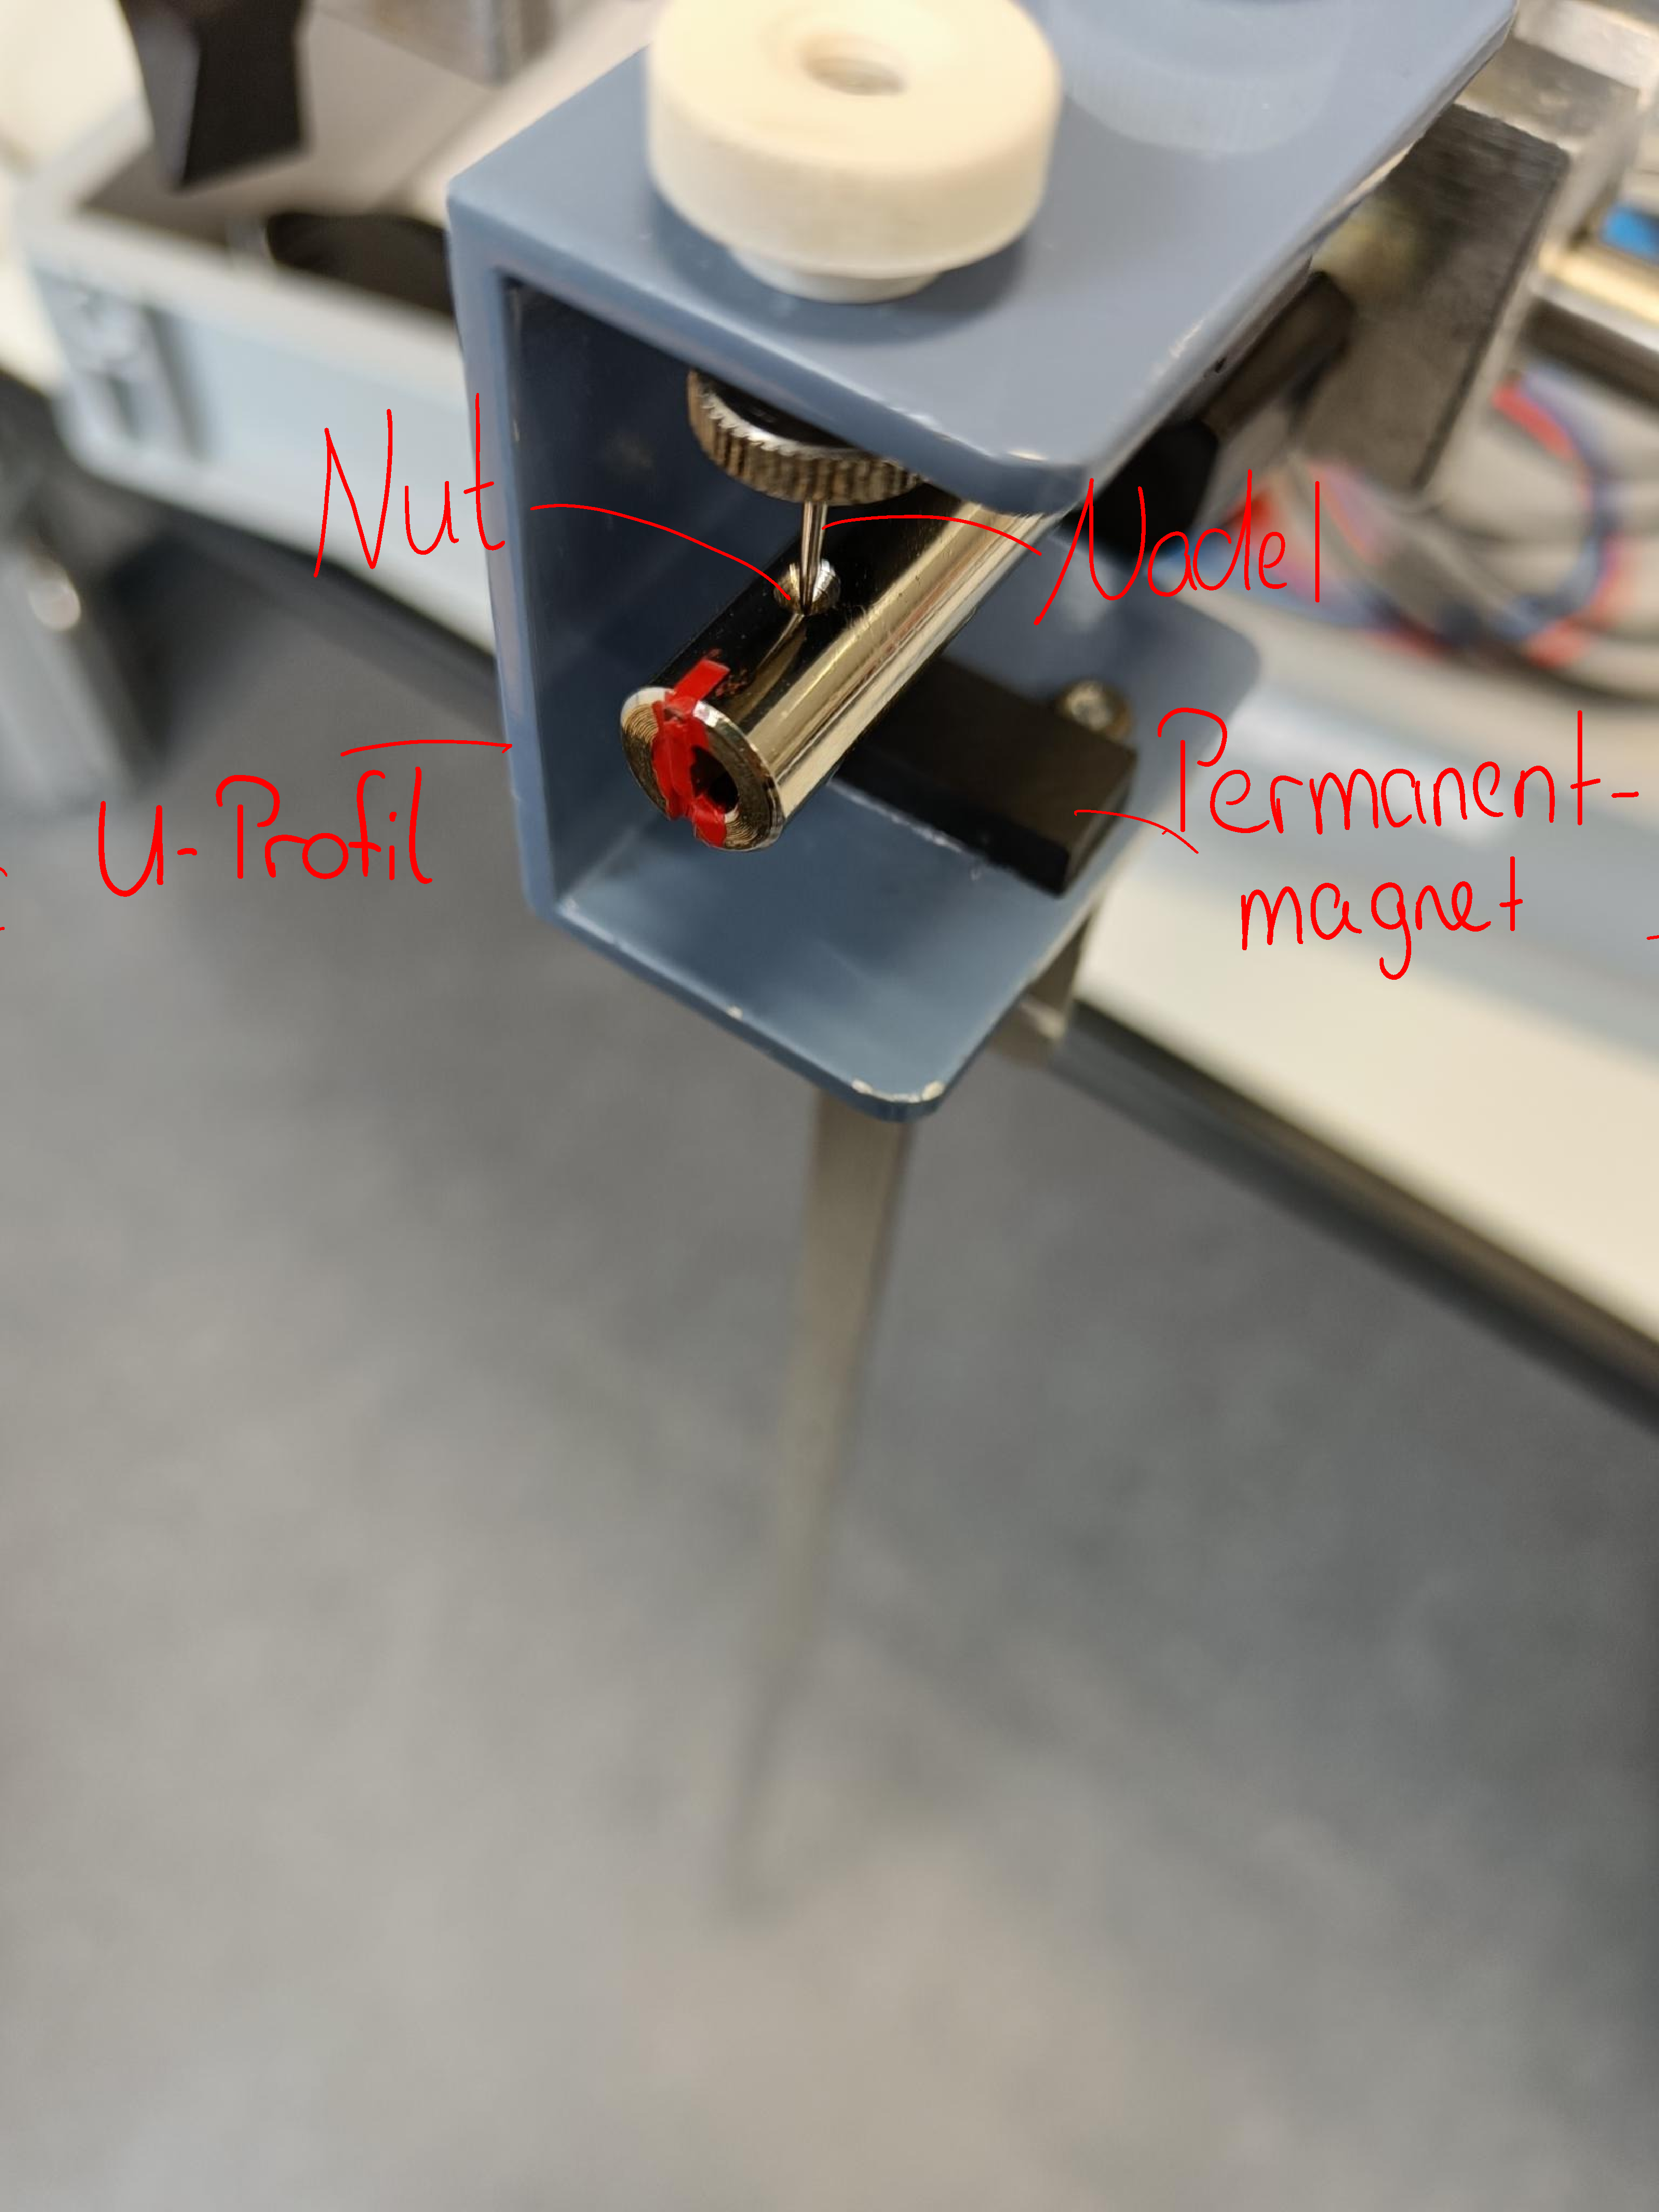
\includegraphics[width=0.7\textwidth]{Bilder/Nahaufnahme-Nut_B.pdf}
    \caption{Nahaufnahme von der Nut mit Nadel}
\end{figure}
In dem Bild oben können sie sehen, wie die Nadel des U-Profils in der Nut des Winkelaufnehmers liegt.

Ein Pendelkörper kann an der Pendelstange befestigt werden, indem man die Stange in diesen schiebt, und mit der Schraube des Pendelkörpers festzieht.\\
\subsection{Durchführung}
Zu beginn des Versuchs haben wir das 3-Bein Stativ aufgebaut wie oben beschrieben. 
Hier sind wir sicher gegangen, dass dieses Fest ist, und haben zur Überprüfung an diesem gewackelt.
Mit der Wasserwaage haben wir überprüft, dass die vordere Stange horizontal ist. 
Dann haben wir beide Winkelaufnehmer mit einer Kreuzmuffe befestigt, Später haben wir diese noch weiter auseinander gerückt, da sich sonst die Pendel in die Quere gekommen wären. 
Mit der Wasserwaage haben wir überprüft, dass der Winkelaufnehmer horizontal ist. 
Diesen haben wir stark befestigt, dass das Gewicht des Pendelkörpers diesen später nicht verdreht.
 
Die Pendelstange haben wir an dem U-Profil mit den davor vorgesehenen Schrauben festgeschraubt, und dieses dann mit den Nadeln in die Nut des Winkelaufnehmers gestellt.\\
Vor beginn der Messung haben wir den Winkelaufnehmer genullt. 
Wir haben beide Winkelaufnehmer an CASSY angeschlossen, um zu überprüfen, welchen wir besser Nullen können.
Hierfür haben wir den Winkelaufnehmer in die Steckdose eingesteckt, und an dem Drehregler des Geräts gedreht, bis bei CASSy ungefähr null Volt angezeigt wurden.
Der auf den Bildern und Skizzen linke Winkelaufnehmer konnten wir besser nullen, weswegen wir diesen für die weiteren Messungen verwendet haben.
Den Winkelaufnehmer haben wir an Input A des CASSY angeschlossen\\
\begin{figure}[H]
    \centering
    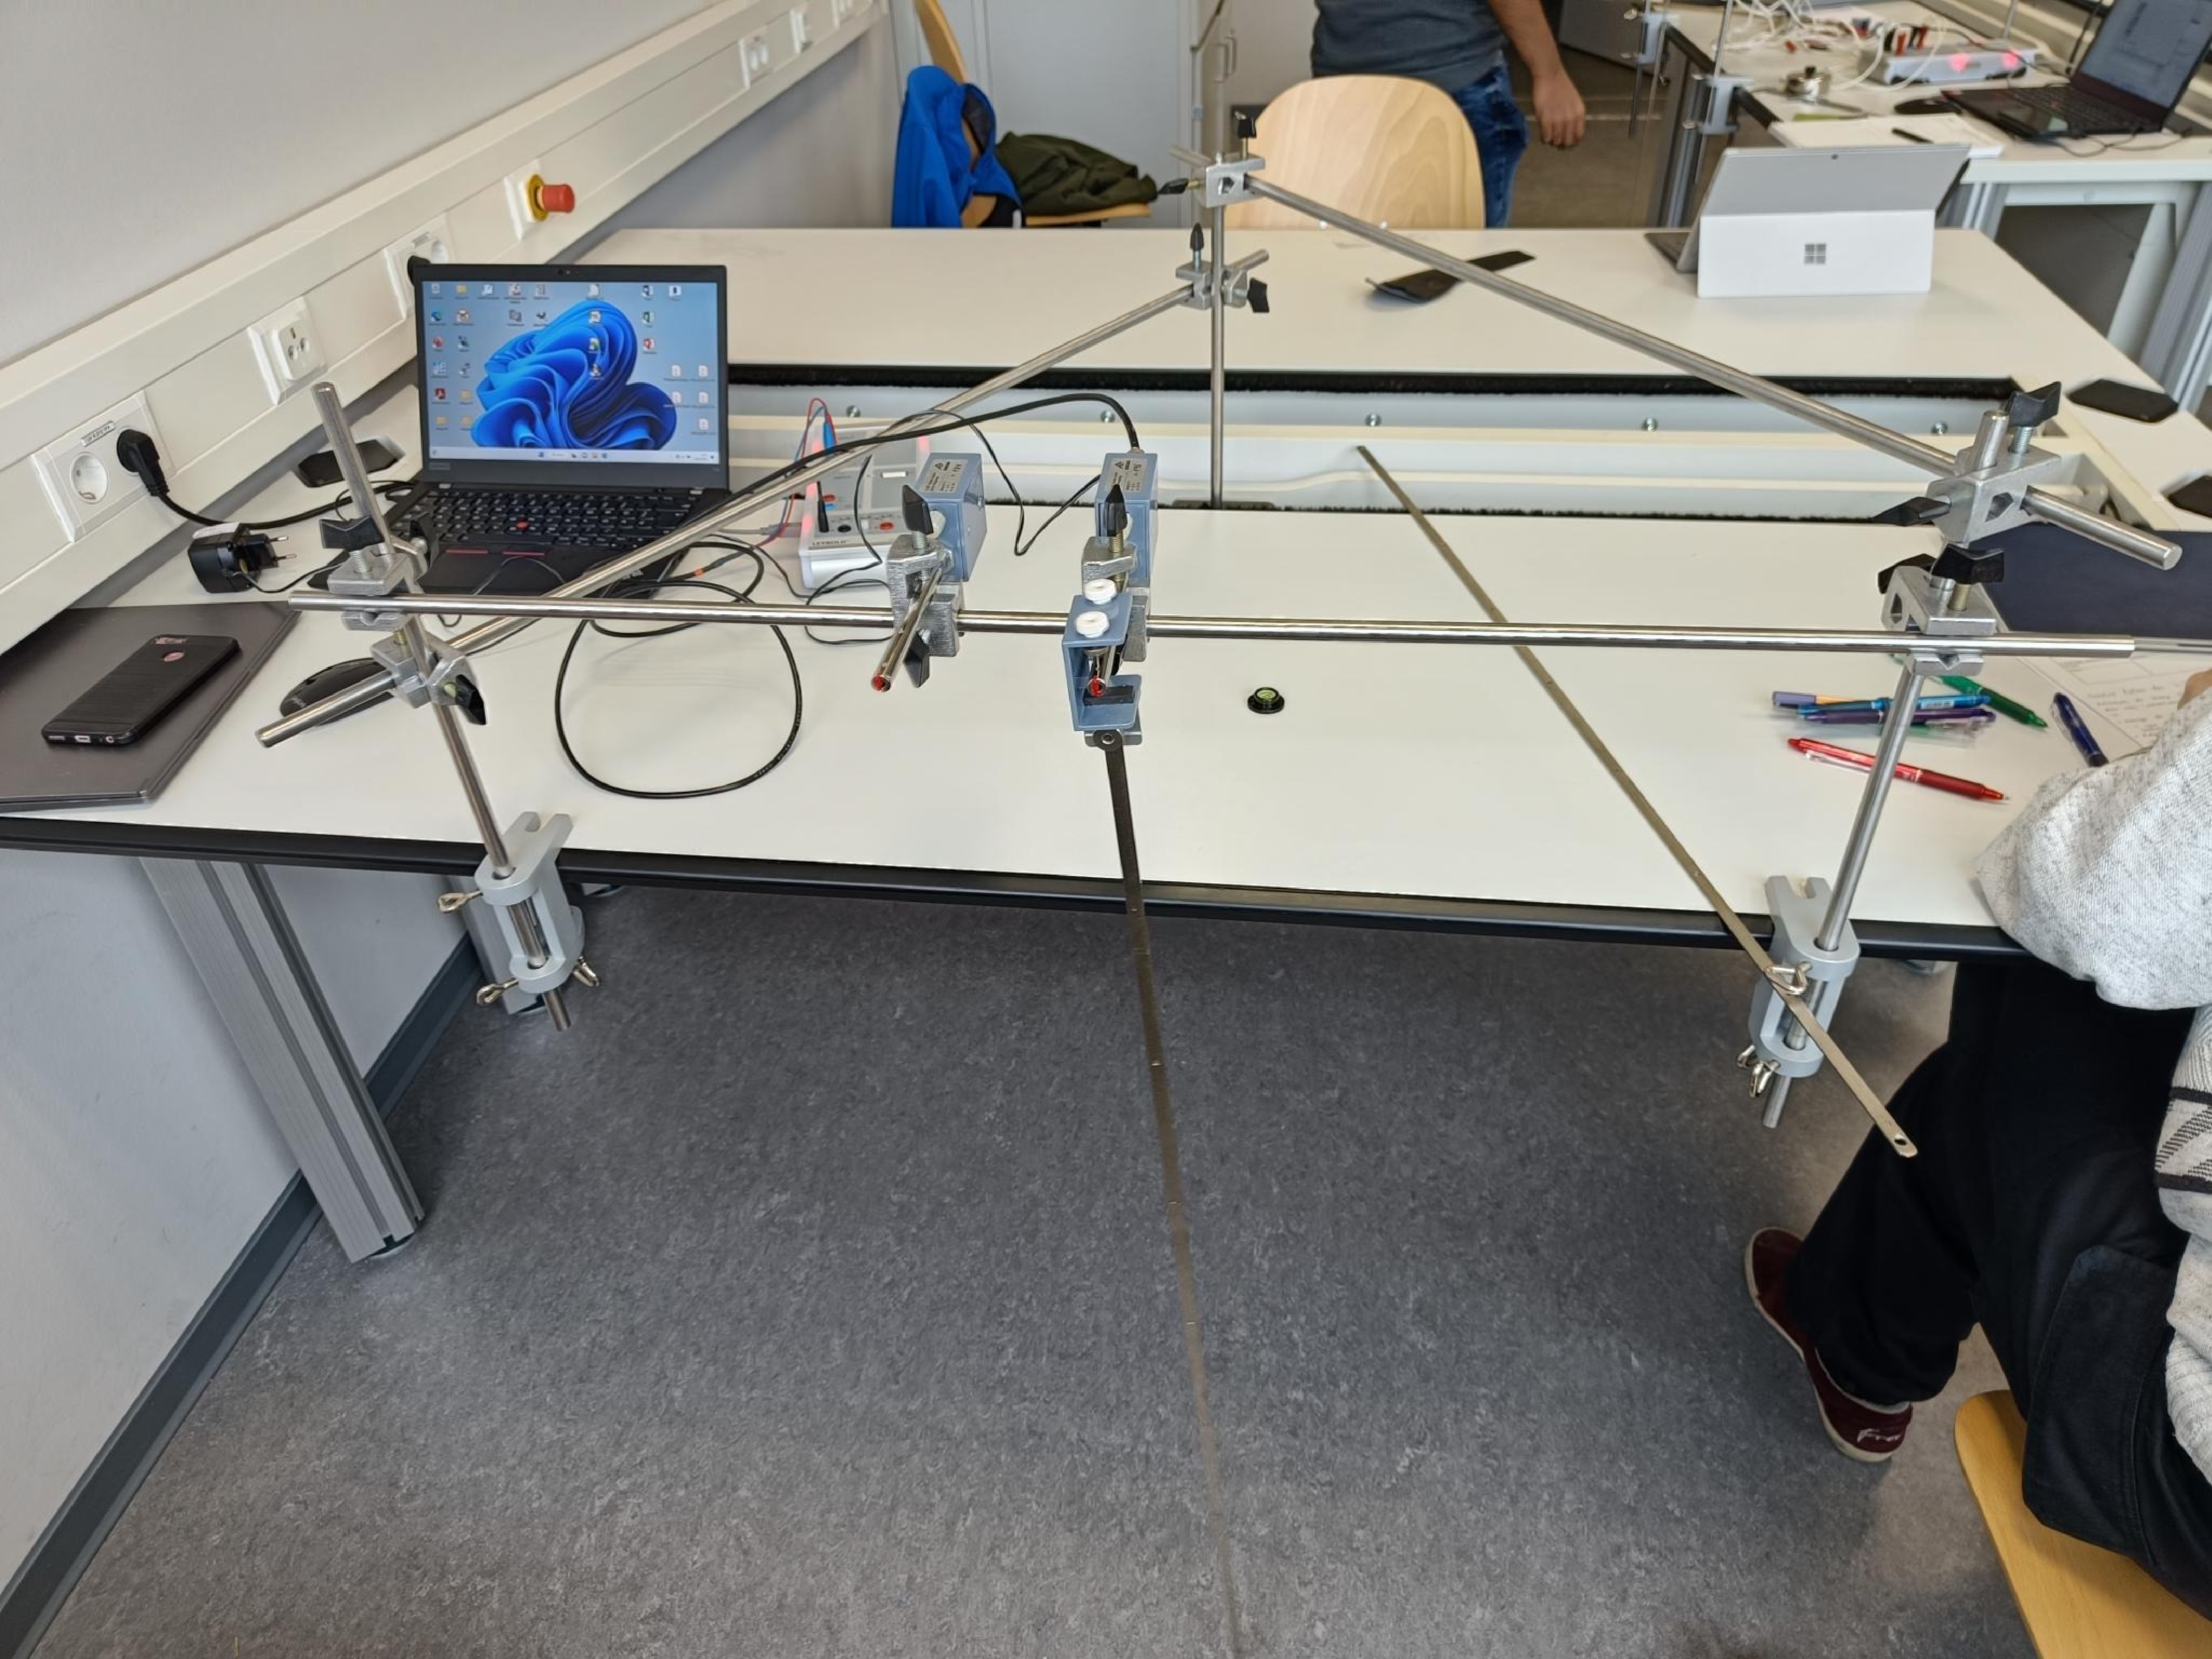
\includegraphics[width=0.7\textwidth]{Bilder/gesamtaufbau.pdf}
    \caption{Bild des Gesamtaufbaus}
    \end{figure}
Hier ein Bild des Gesamtaufbaus. Zu sehen ist das 3-Bein Stativ und das Daran befestigte Pendel.
In diesem betrachten wir das Pendelverhalten der weiten Stange welche wir nicht gewählt haben.\\

Da unsere Kleinwinkelnäherung bis Maximal 5° geht, haben wir ausgerechnet, um welche Strecke am Boden das Pendel ausgelenkt werden darf sodass wir unter 5° bleiben. 
Diese Auslenkung haben wir mit einem Geodreieck auf dem Boden gemessen. 
Die Maximale Auslenkung war 9cm weswegen wir unser Pendel 7cm Ausgelenkt haben.
Bei einer Auslenkung von 7cm hatten wir eine Spannung zwischen -0.4V und 0.4V weswegen wir den Messbereich auf -1V bis 1V gestellt haben.\\

Zur Bestimmung der Messwerterfassungseinstellungen haben wir erst eine Testmessung über wenige Schwingungsperioden durchgeführt, um zu überprüfen wie gut ablesbar die Maxima sind.
Unser erstes Messintervall war 20ms, Mit diesem Konnten wir die Maxima schon gut ablesen, bei einem Messintervall von 10ms war dies jedoch besser.\\
Wir haben ebenfalls die zweite Pendelstange aufgehangen und überprüft wie gut ablesbar bei dieser die Maxima sind.
 Diese waren unsauberer, was daran liegen könnte, dass die Stange gebogen war, und die Schwingung dadurch nicht so gleichförmig abgelaufen ist.
 Diese Vergleichsmessung haben wir unter Test-Vergleich-01 abgespeichert. \\

 Als nächstes haben wir das Pendel in drei Abschnitte eingeteilt in welche wir die Länge des Pendels messen. 
 Die genaue Aufteilung mit Skizze wird in de Rohdaten noch genauer beschrieben. Kurz zusammengefasst messen wir den Abstand zwischen den Nadeln und U-Profil Boden ($l_1$).
Vom U-Profil Boden bis zur ersten Einkerbung der Pendelstangen Halterung ($l_2$) und von dort bis zum Mittelpunkt des Pendelkörpers ($l_3$).
$l_1$ und $l_2$ sind Strecken die gut mit dem Messschieber gemessen werden können, da man diese gut ansetzen kann. 
Von der ersten Einkerbung konnte man das Maßband gut hängen lassen.
Für $l_1$ und $l_2$ haben wir die Messungen vor dem Pendeln durchgeführt. 
Wir haben jede Strecke 3 mal gemessen. Den Abstand zwischen Nadel und U-Profil Boden haben wir pro Nadel 3 mal gemessen.
Vor dem Messen mit dem Messschieber haben wir diesen komplett zusammen geschoben und überprüft, ob dieser dann null anzeigt. 
So konnten wir überprüfen, ob dieser ein Kalibrirungsfehler hat.
Das dies der Fall war, können wir davon ausgehen, dass wir keinen systematischen Fehler auf das Messen mit dem Messschieber haben.\\

Dann haben wir die erste Messung gestartet. 
Die Messung haben wir Manuell gestartet, also ohne Trigger, sodass wir anfängliche Störungen vom Auslenken des Pendels nicht aufzeichnen. 
Wir haben jede Messung von Hand abgebrochen nach ca. 185 Sekunden. 

\begin{table}[H]
        \centering
        \begin{tabularx}{1.0\textwidth}{X X X X} % adjust width as needed
            \toprule
            \textbf{Intervall} & \textbf{Messzeit} & \textbf{Trigger} & \textbf{Bereich} \\
            \midrule
            1ms & 185s & kein Trigger & -1V bis 1V \\
            \bottomrule
        \end{tabularx}
        \caption{Messwerterfassungseinstellungen}
        \label{tab:mytable}
    \end{table}

Hier eine Übersicht unserer Messwerterfassungseinstellungen.\\
Das Penel haben wir mit der Hand ca. 7cm ausgelenkt, dies haben wir mit dem Geodreieck gemessen (Auf Bild unten zu sehen). 
Bei jeder Messung haben wir versucht in etwa die gleiche Auslenkung zu haben. 
Das pendel sollte möglichst störungsarm losgelassen werden, um mögliche Effekte des Starten zu minimieren. 
Falls das Pendel zu sehr hin und her gewackelt hat, haben wir die Messung abgebrochen und neu gestartet.\\
\begin{figure}[H]
    \centering
    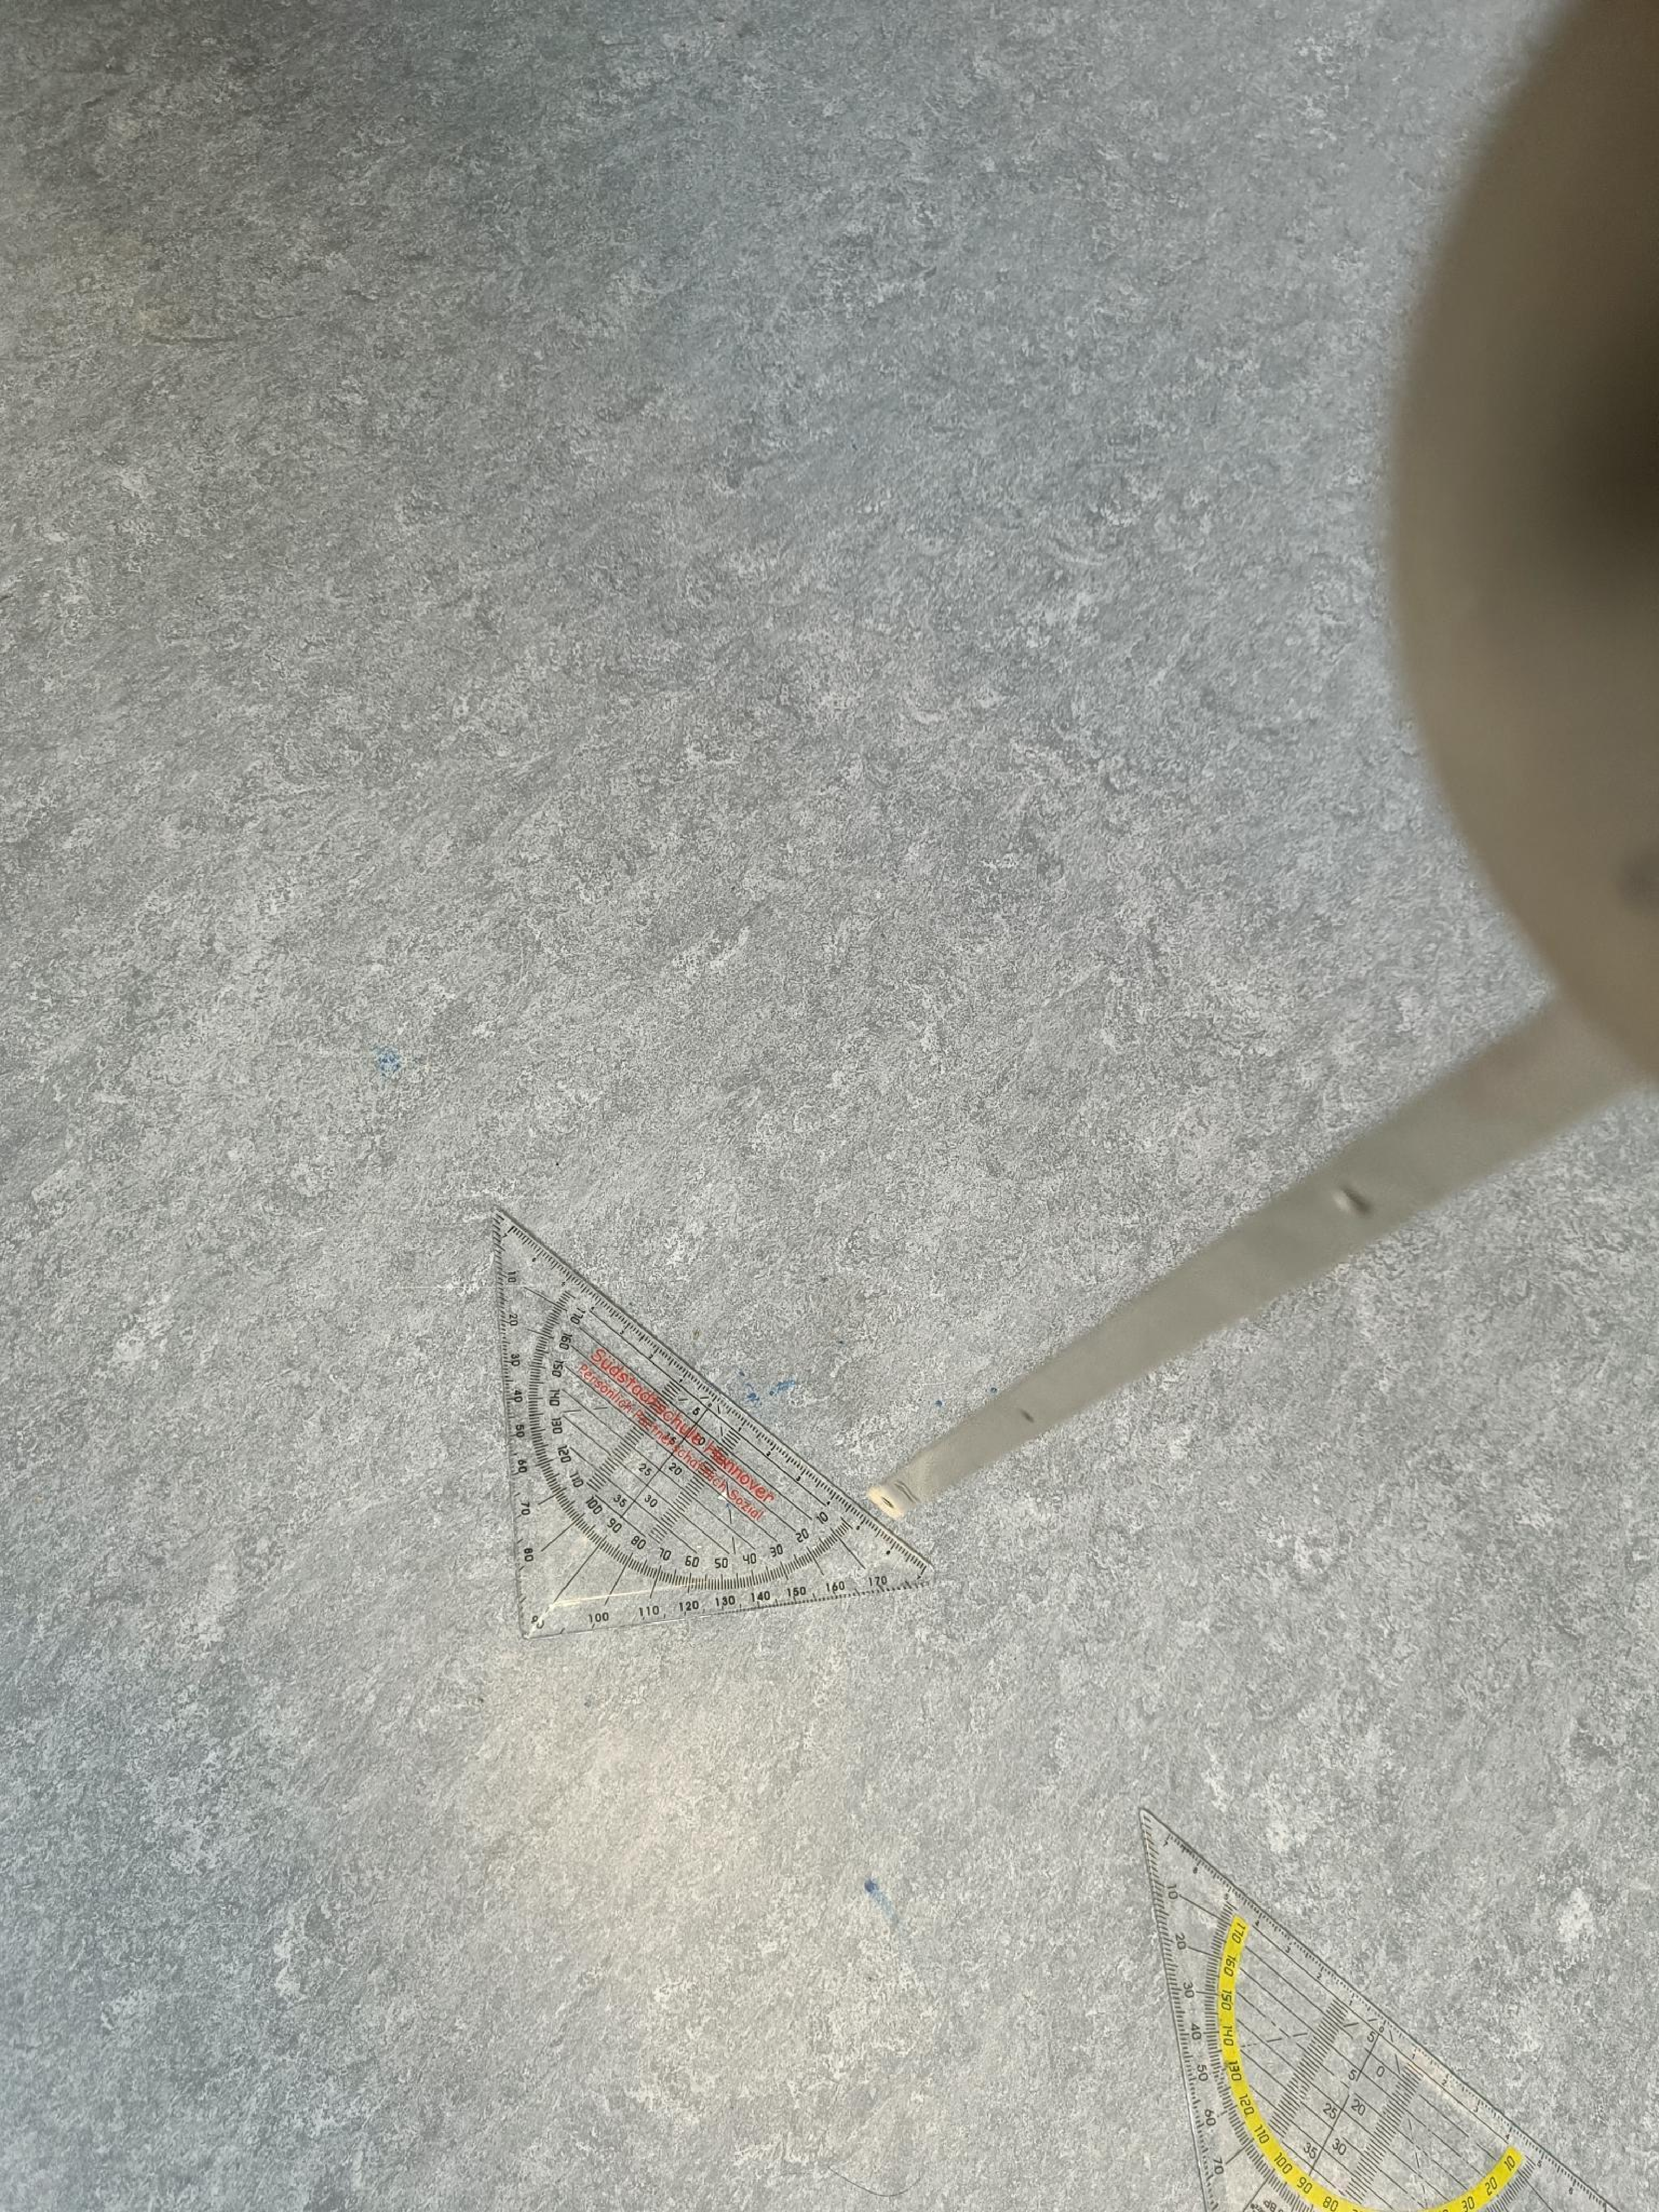
\includegraphics[width=0.7\textwidth]{Bilder/geodreieck.pdf}
    \caption{Bestimmung der Auslenkung mit Geodreieck}
    \end{figure}
Die Messung nur mit der Pendel Stange haben wir insgesamt drei mal durchgeführt. 
Für jede dieser Messungen haben wir die Periodendauer überschlagen.
Wir haben den Zeitpunkt des ersten Maximums mit dem Peakschwerpunkt bestimmt. Das selbe haben wir mit dem zwanzigsten Maximum getan. 
Die Periodendauer haben wir dann mit der folgenden Formel bestimmt.
\begin{equation}
T = \frac{t_{20} - t_{1}}{19}
\end{equation}
Bei der Rechnung nach nach der Messung haben wir durch die falsche Periodenzahl (20) geteilt. 
Dies ist uns aufgefallen, als wir g bestimmt haben, weshalb wir unsere Rechnungen für die Periodendauer wiederholt haben.\\

Nachdem wir diese durchgeführt haben, haben wir den Pendelkörper an der Pendelstange befestigt. 
Und das Pendel erneut auf gehangen. 
Diesmal waren wir beim aufhängen besonders vorsichtig, das die Masse des Pendels nun um einiges größer war, und somit den Winkelaufnehmer verdrehen könnte
An den anderen Winkelaufnehmer haben wir die andere Pendelstange gehangen, und beide Pendel ausgelenkt.
Nach Augenmaß haben wir überprüft, ob diese ungefähr die gleiche Frequenz haben. Und haben gegebenenfalls Die Position des Pendelkörpers angepasst.
Wenn dass Pendel mit Pendelkörper eine kleinerer Periodendauer hat, muss der Pendelkörper nach unten bewegt werden, wenn es eine größere Periodendauer hat nach oben.
Diese Justierungen haben wir durchgeführt, bis die Frequenz augenscheinlich übereingestimmt hat. \\

Danach haben wir mit CASSY einige Schwingungsperioden (zwischen 10 und 50) aufgenommen um zu überprüfen, ob die Frequenzen der beiden übereinstimmen. 
Hierfür haben wir die Lage der Maxima der beiden Schwingungen (Schwingung mit Pendelkörper und ohne) verglichen.
Ob deren relative position zueinander im Verlauf der Messung gleich geblieben ist.
Hier haben wir den Pendelkörper ebenfalls einige male neu justiert und den Vergleich erneut durchgeführt bis die relative Position der Maxima gleich geblieben sind.\\

Mit dieser Pendelkörperposition haben wir dann eine gesamte Messung durchgeführt.
Dies haben wir gleich wie bei dem Pendel ohne Pendelkörper gemacht. Wir haben wieder 185 Sekunden aufgezeichnet. 
Daraus haben wir ebenfalls die Periodendauer überschlagen. 
Dies haben wir auf die gleiche weise getan wie ohne Pendelkörper. Wobei wir wieder durch 20 geteilt haben.

\subsection{Übereinstimmung der beiden Pendel}

Zur genauen Überprüfung der Übereinstimmung der Periodendauern haben wir uns die relative Position der Maxima am Anfang der Messung angeschaut, und die relative Position der Maxima am Ende der Messung. 
Mit dieser Relativen Position konnten wir die Verschiebung pro Periodendauer bestimmen.
Hierfür haben wir den Peakschwerpunkt des ersten Maxima der ersten Messung mit bzw. ohne Pendelkörper bestimmt. 
So wie den Peakschwerpunkt der letzten Maxima. 

\begin{figure}[H]
    \centering
    \subfloat[Position der Messungen zueinander am Anfang]{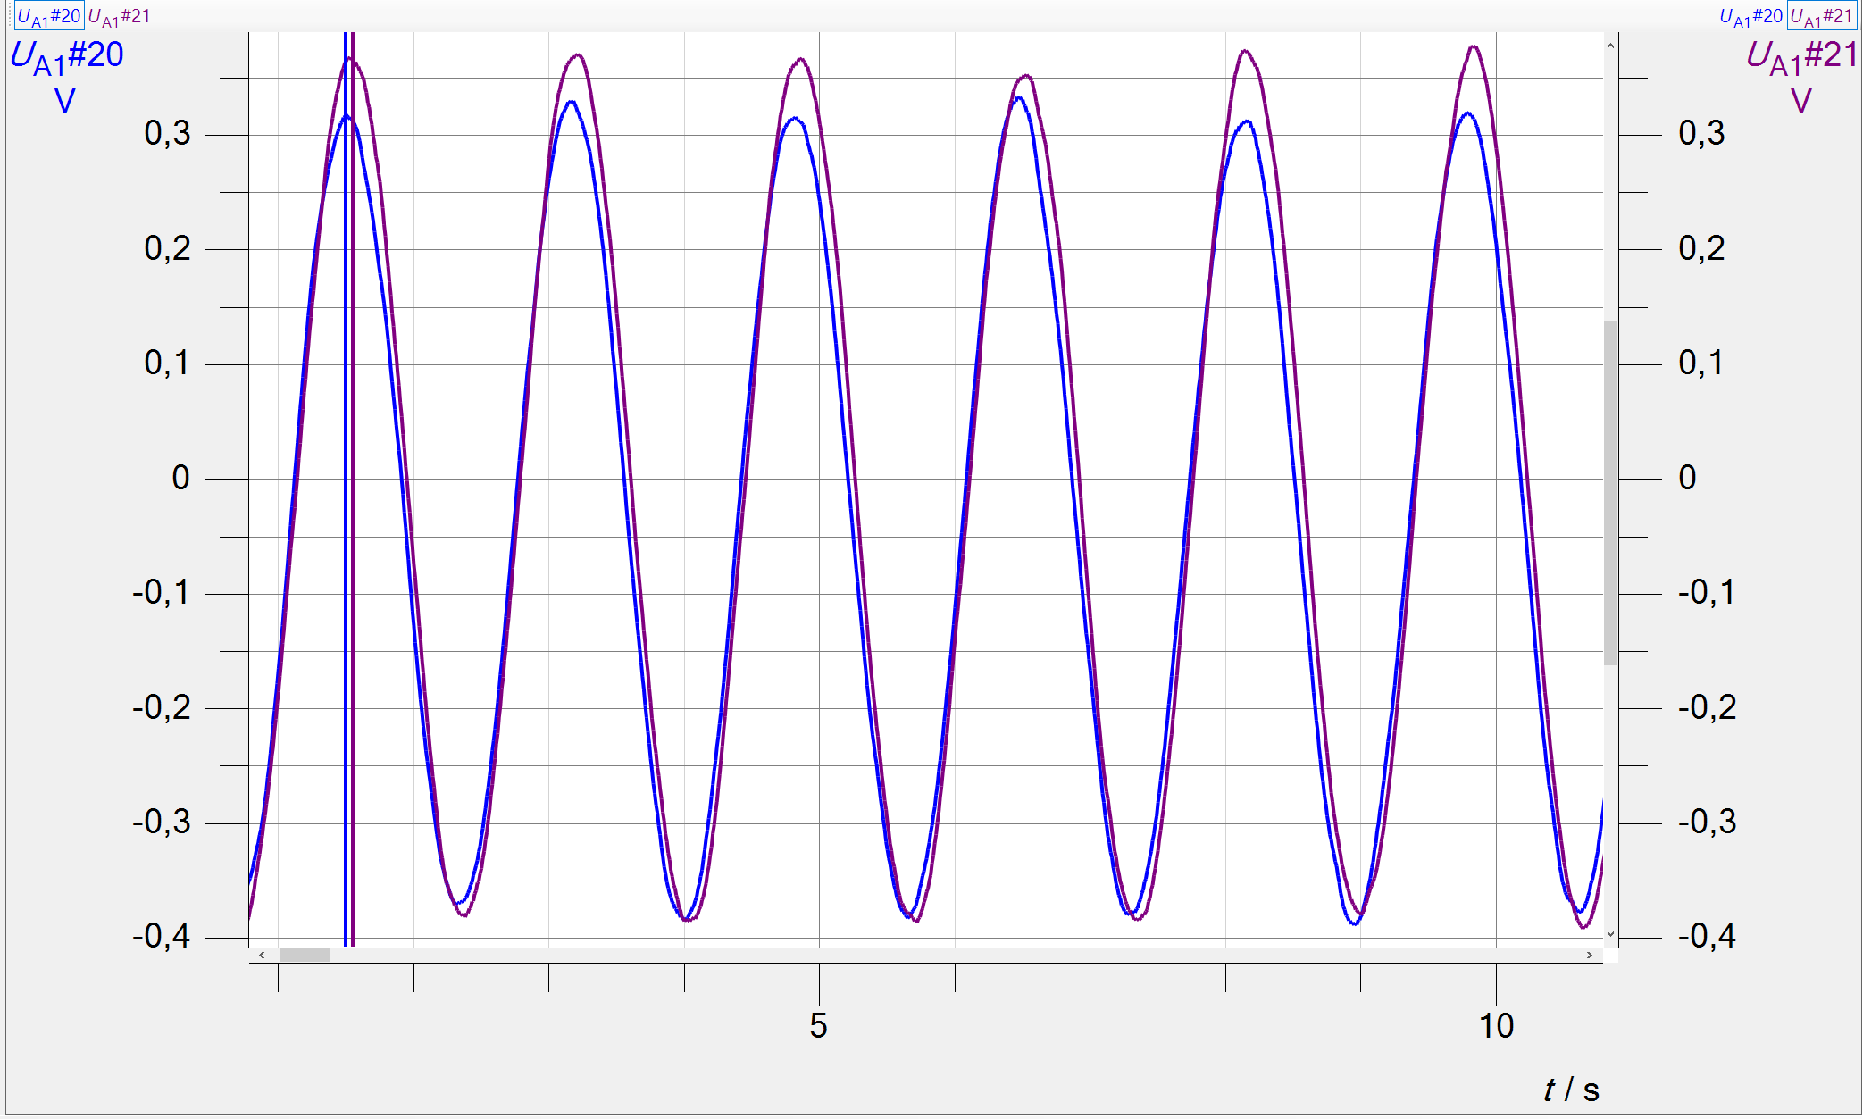
\includegraphics[width=0.8\textwidth]{plots/Verschiebung-Anfang.pdf}}
    \hfill
    \subfloat[Position der Messungen zueinander am Ende]{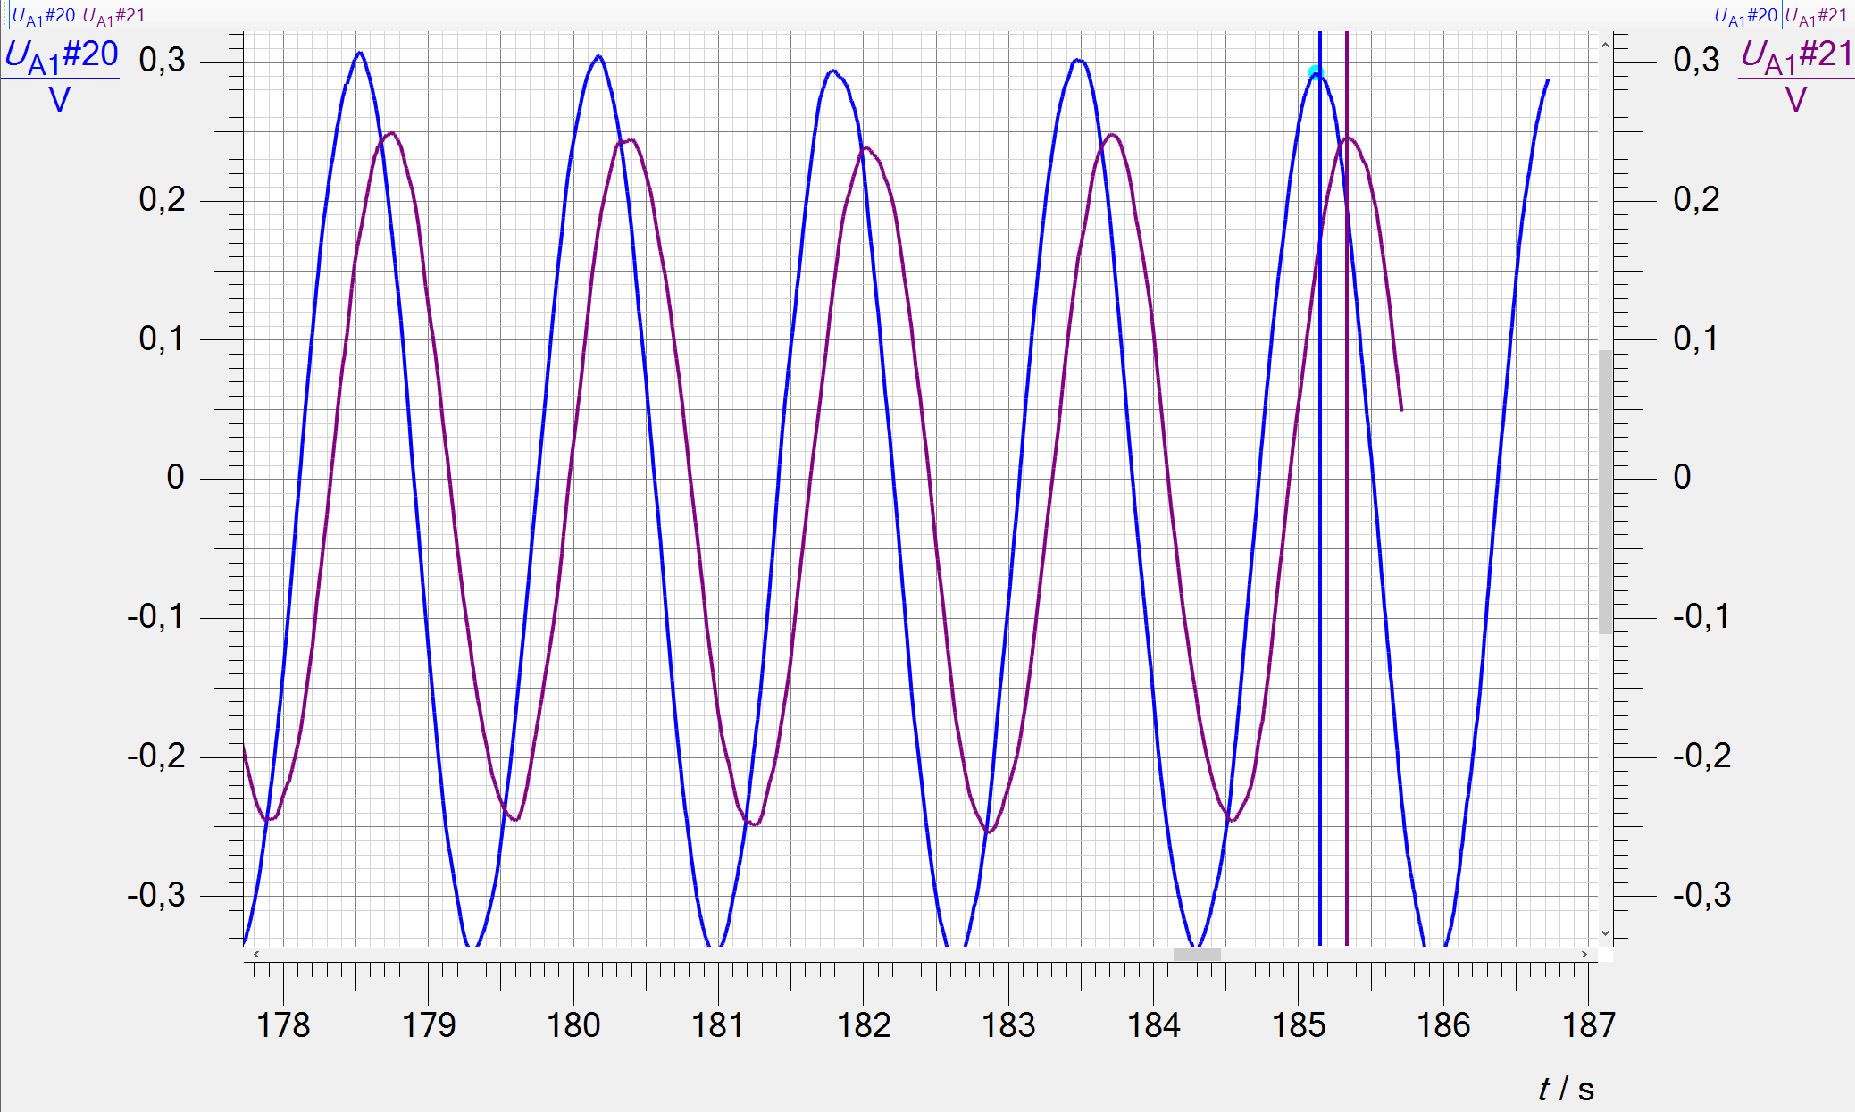
\includegraphics[width=0.8\textwidth]{plots/Verschiebung-ende.pdf}}
    \caption{Graphen zu Bestimmung der Verschiebung}
    \end{figure}

In den Graphen ist in Violett die Erste Messung der Schwingung ohne Pendelkörper zu sehen.
In blau ist die erste Messung mit Pendelkörper zu sehen. 
Der obere Graph zeigt die position der zwei Schwingungen zueinander am Anfang der Messung. 
Hier ist bei dem ersten Maxima für beide Schwingungen der Peak mit dem Schwerpunktartig eingezeichnet. 
Für den Violetten Graph ($t_v$) und für den blauen Graph ($t_b$) konnten wir so die Zeitpunkte ablesen. 
Das gleiche haben wir am Ende der Messung getan (unterer Graph).
Daraus ergibt sich:
\begin{center}
$t_{v_a}$ = 1.552s \qquad $t_{v_e}$ = 185.331s\\
$t_{b_a}$ = 1.499s \qquad $t_{b_e}$ = 185.148s
\end{center}

aus diesen Werten können wir die zeitliche Verschiebung pro Periode berechnen, indem wir zunächst $ \Delta t_a = t_{v_a}-t_{b_a}$ und $ \Delta t_e = t_{v_e}-t_{b_e}$ berechnen.
Daraus können wir $ \Delta t = \Delta t_e - \Delta t_a $ berechnen was die Verschiebung über die gesamte Messzeit ist.
Wir haben in diesen Messungen insgesamt 114 Maxima, weshalb wir dieses $\Delta t$ durch 113 teilen müssen, um die Verschiebung pro Periode zu bestimmen. 
Daraus ergibt sich:
\begin{center}
$\Delta t $ = 0.13s \qquad und pro Periode \quad $\Delta t_P$ = 0.00115s
\end{center}
Mit der überschlagenen Periodendauer von T = 1.6559s Aus der Messung der Stange, ergibt das eine relative Abweichung pro Periode von 0.07\% 

Die relative Verschiebung mit weniger als 1 Promille pro Periode ist gut weshalb wir mit dieser Pendelposition weiter gemessen haben.
Da die Periodendauern übereingestimmt haben, haben wir mit dieser Position zwei weitere Messungen durchgeführt.
Für diese haben wir jedes mal die Periodendauer überschlagen.\\

Zur Messung des Durchmessers, haben wir das Pendel vom Winkelaufnehmer genommen und mit dem Messschieber den Durchmesser gemessen.
Wir haben darauf geachtet, dass er möglichst mittig positioniert war, und wir in drei verschiedenen Positionen gemessen haben. \\

Den Abstand vom Pendelkörpermittelpunkt bis zu der ersten Einkerbung der Pendelaufhängung haben wir in hängendem Zustand mit dem Maßband gemessen ($l_3$).
Wir haben das Maßband gerade runter hängen lassen sodass es nicht gebogen ist. 
Durch die Messung mit dem Messschieber wussten wir, dass der Mittelpunkt 4.040cm unter der oberen Kante war.
Wir haben die Position das Maßband sowohl nach Augenmaß mit dem Mittelpunkt verglichen, als auch geschaut, 
dass der Punkt an welchem wir ablesen 4.040cm unterhalb dem oberen Pendelkörper Rands ist.

Auch diese Messung haben wir drei mal durchgeführt.\\
Im Nachhinein ist uns aufgefallen, dass dies keine sehr geschickte Wahl war, da wir eh den Radius des Pendelkörpers mit der Messschieber bestimmt haben.
Eine höhere Genauigkeit hätten wir erzielen können, wenn wir nur bis zu der Oberseite des Pendels gemessen hätten. 

Zuletzt haben wir dann eine Überschlagsrechnung für g gemacht. Dies haben wir mit Formel \ref{eq:formel} gemacht.
Da wir kein sinnvolles Ergebnis erhalten haben, ist uns aufgefallen, dass in der Vorherigen Berechnung von T einen Fehler gemacht haben. 
So konnten wir unsere Rechnung für T korrigieren und g erneut bestimmen. Da dieses Ergebnis mit unseren Erwartungen (von ca. 9.81$m/s^2$) übereinstimmt haben wir den Versuch beendet.

\begin{aufgabe}{Rohdaten}
  Stellen Sie Ihre Rohdaten dar, tabellarisch für $l_p$ und $r_p$,
  grafisch für den Verlauf der Schwingung der Stange ohne Pendelkörper
  sowie der Pendelschwingung (für mindestens drei Messreihen).
\end{aufgabe}

\section{Rohdaten}
Zur Bestimmung der Pendellänge haben wir das Pendel in verschiedene Teilstücke unterteilt, damit wir diese Möglichst genau messen können. 
Dies Abschnitte haben wir so gewählt, dass wir diese mit dem jeweiligen Messinstrument möglichst exakt bestimmen können. 

\begin{figure}[H]
    \centering
    \subfloat[Skizze U-Profil mit Längenabschnitten]{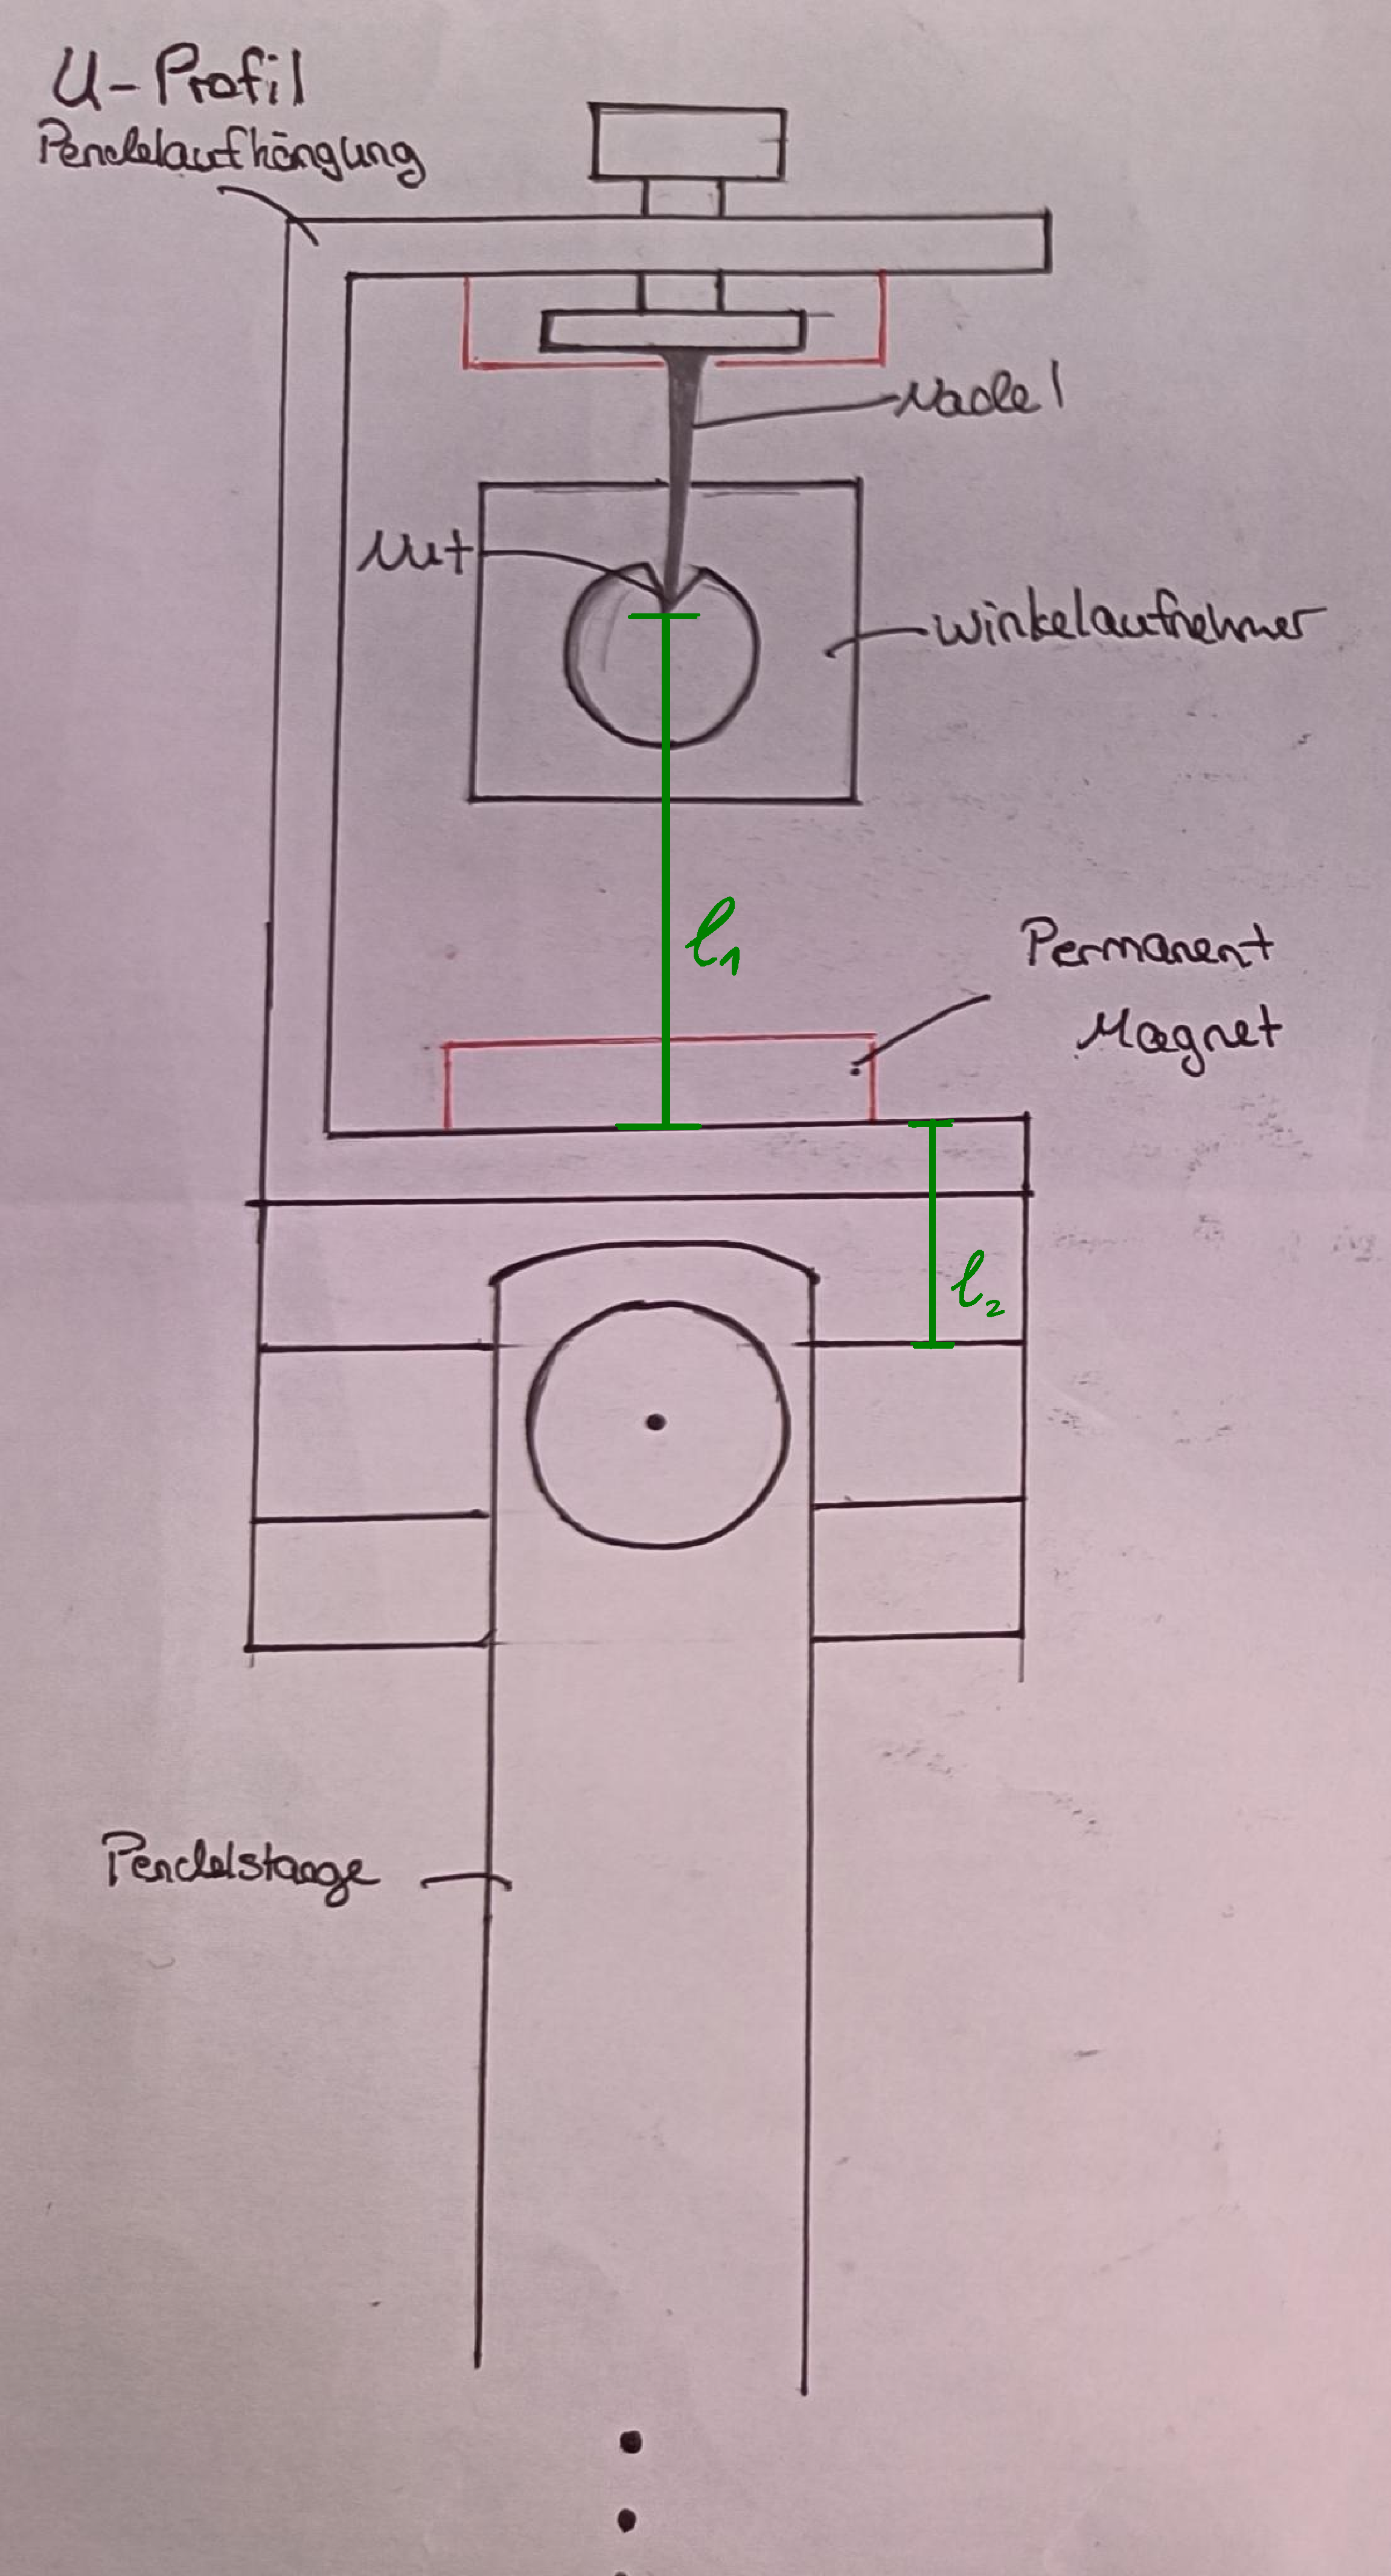
\includegraphics[width=0.45\textwidth]{Bilder/u-profiel-L.pdf}}
    \hfill 
    \subfloat[Skizze des Gesamten Pendel mit Längenabschnitten]{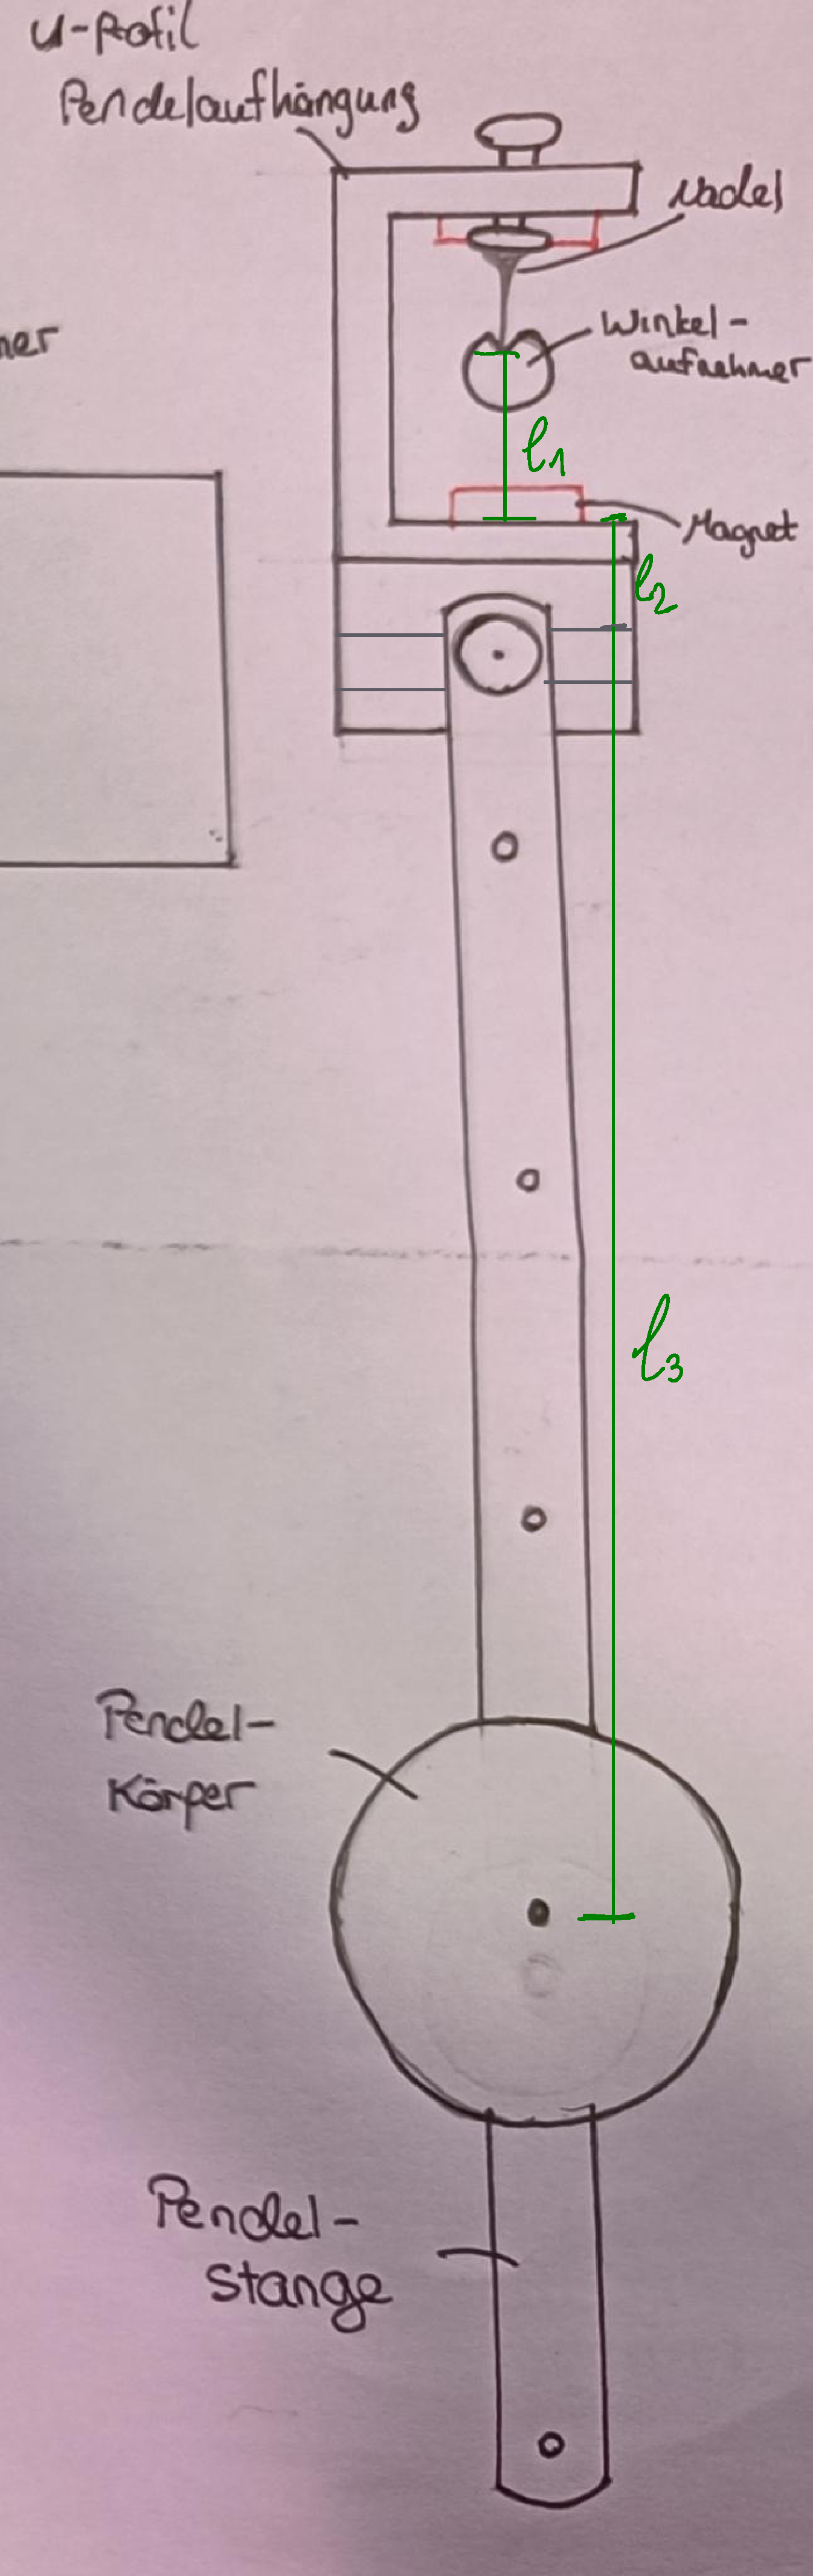
\includegraphics[width=0.3\textwidth]{Bilder/pendel-gesamt-L.pdf}}
    \label{Pendel Aufbau}
\end{figure}
In den beiden Skizzen ist zu sehen wie wir die Längenabschnitte gewählt haben. 
Hier ist zu beachten, dass die Zeichnung nicht Maßstabsgetreu ist.
$l_1$ ist der Abstand zwischen Nadelspitze und dem Boden des U-Profils. 
Dies haben wir mit der Schieblehre gemessen, wären die Pendelstange noch nicht montiert war und das U-Profil nicht auf gehangen.\\

$l_2$ bezeichnet den Abschnitt zwischen dem Boden des U-Profils und der ersten Einkerbug der Pendelaufhängung.
$l_3$ ist der Abstand zwischen der Ersten Einkerbung bis zum Mittelpunkt des Pendelkörpers.\\ 

Da das U-Profil zwei Nadeln hat, haben wir von jeder jeweils den Abstand zum Boden gemessen. 
Die eine Messung bezeichnen wir als $l_1$ die andere als $l_4$.
\begin{figure}[H]
    \centering
    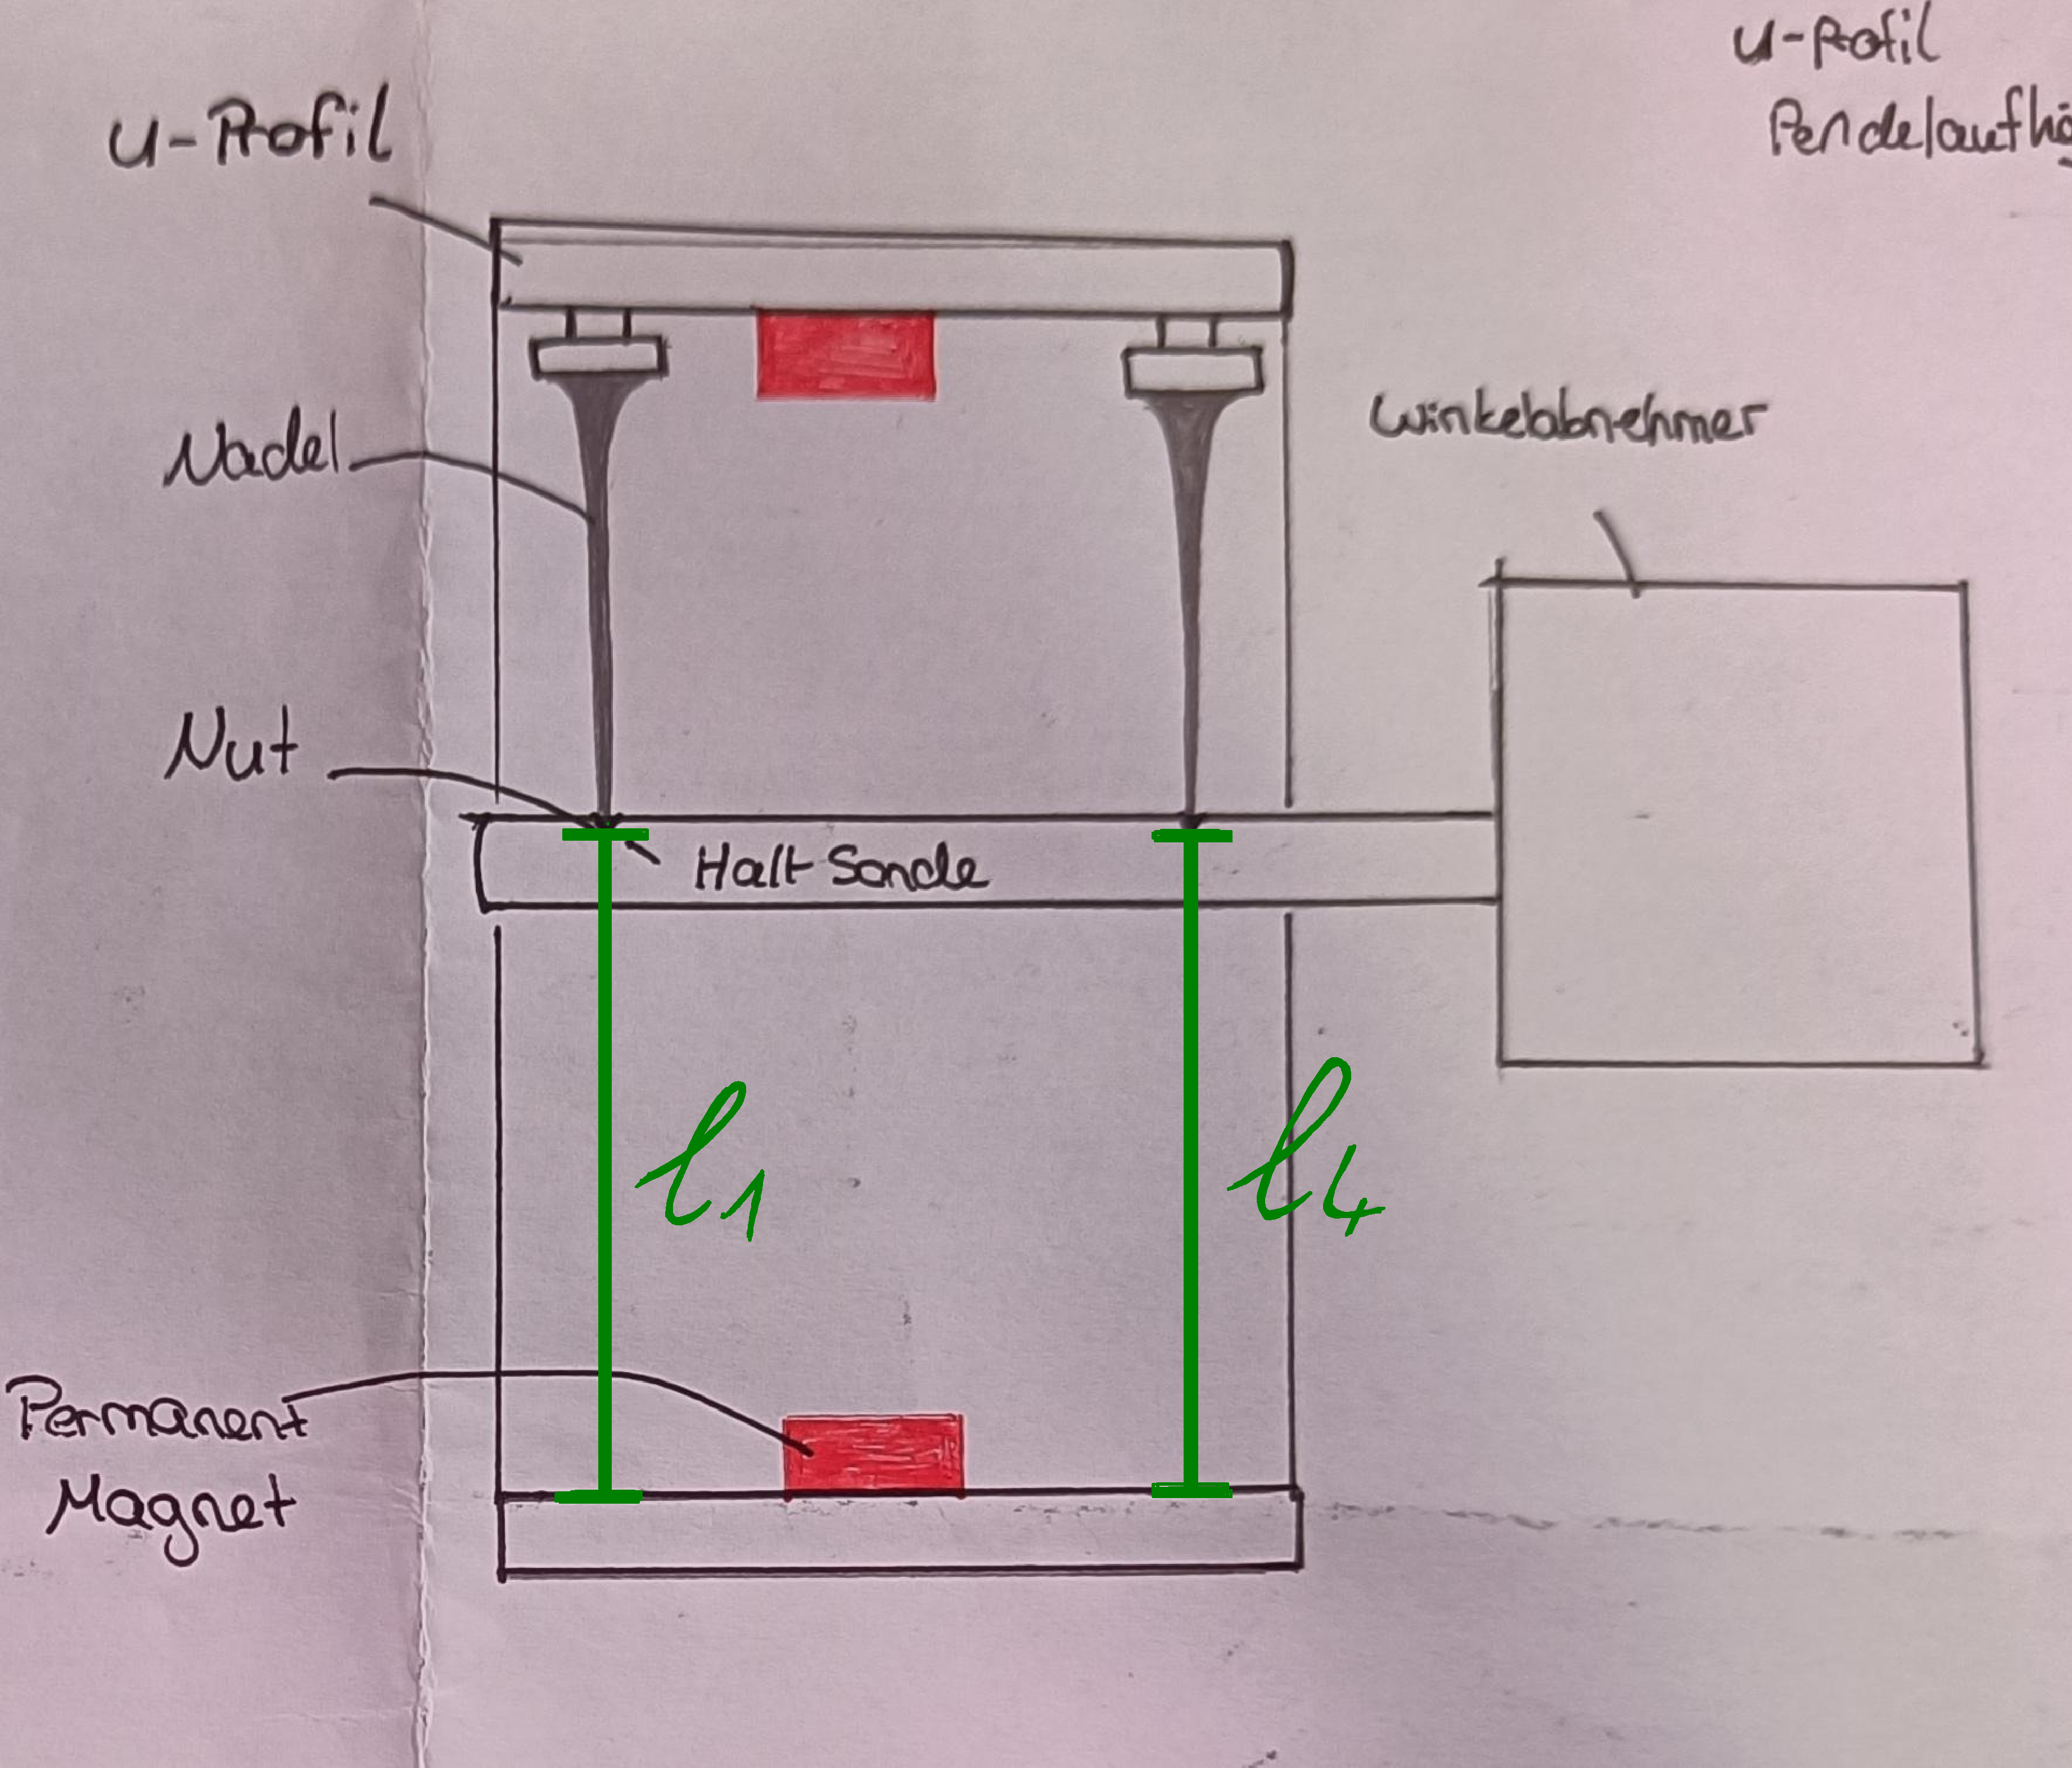
\includegraphics[width=0.45\textwidth]{Bilder/auflage-pende-L.pdf}
    \caption{Skizze des U-Profils mit beiden Nadeln und den Längenabschnitten}
\end{figure}

Für den Radius des Pendelkörpers haben wir den Durchmesser ($d_p$) von diesem bestimmt.
Auf diese Längenmessungen gibt es auch Fehler, hier liegen sowohl systematische Fehler als auch statistische Fehler vor.
Die Systematischen Fehler können den Herstellerangaben entnommen werden für das Maßband. Der Messschieber hat kein Systematischen Fehler.
Die statistischen Fehler können aus der Ablesegenauigkeit bestimmt werden. Diese Fehler werden in der Auswertung genauer diskutiert. 


\begin{table}[H]
        \centering
        \begin{tabularx}{1.0\textwidth}{X l X X} % adjust width as needed
            \toprule
            \textbf{Messung} & \textbf{Längenabschnitt} & \textbf{Wert in cm} & \textbf{Messinstrument} \\
            \midrule
            1. & $l_1$ & 2.595 & Messschieber \\
            2. & & 2.590 &\\ 
            3. & & 2.585 &\\
            \midrule
            1. & $l_2$ & 1.110 & Messschieber \\
            2. & & 1.110 &\\
            3. & & 1.110 &\\
            \midrule
            1. & $l_3$ & 64.2 & Maßband \\
            2. & & 64.2 &\\
            3. & & 64.1 &\\
            \midrule
            1. & $l_4$ & 2.600 & Messschieber \\
            2. & & 2.605 &\\
            3. & & 2.605 &\\
            \midrule
            1. & $d_p$ & 8.080 & Messschieber \\
            2. & & 8.080 &\\
            3. & & 8.080 &\\
            \bottomrule
        \end{tabularx}
        \caption{Tabelle der Längenmessungen}
        \label{tab:längen}
    \end{table}
     
Die Messung der Schwingung ohne Pendelkörper, haben wir insgesamt drei mal durchgeführt.
Für jede haben wir die Schwingungsverläufe aufgezeichnet.
\begin{figure}[H]
    \centering
    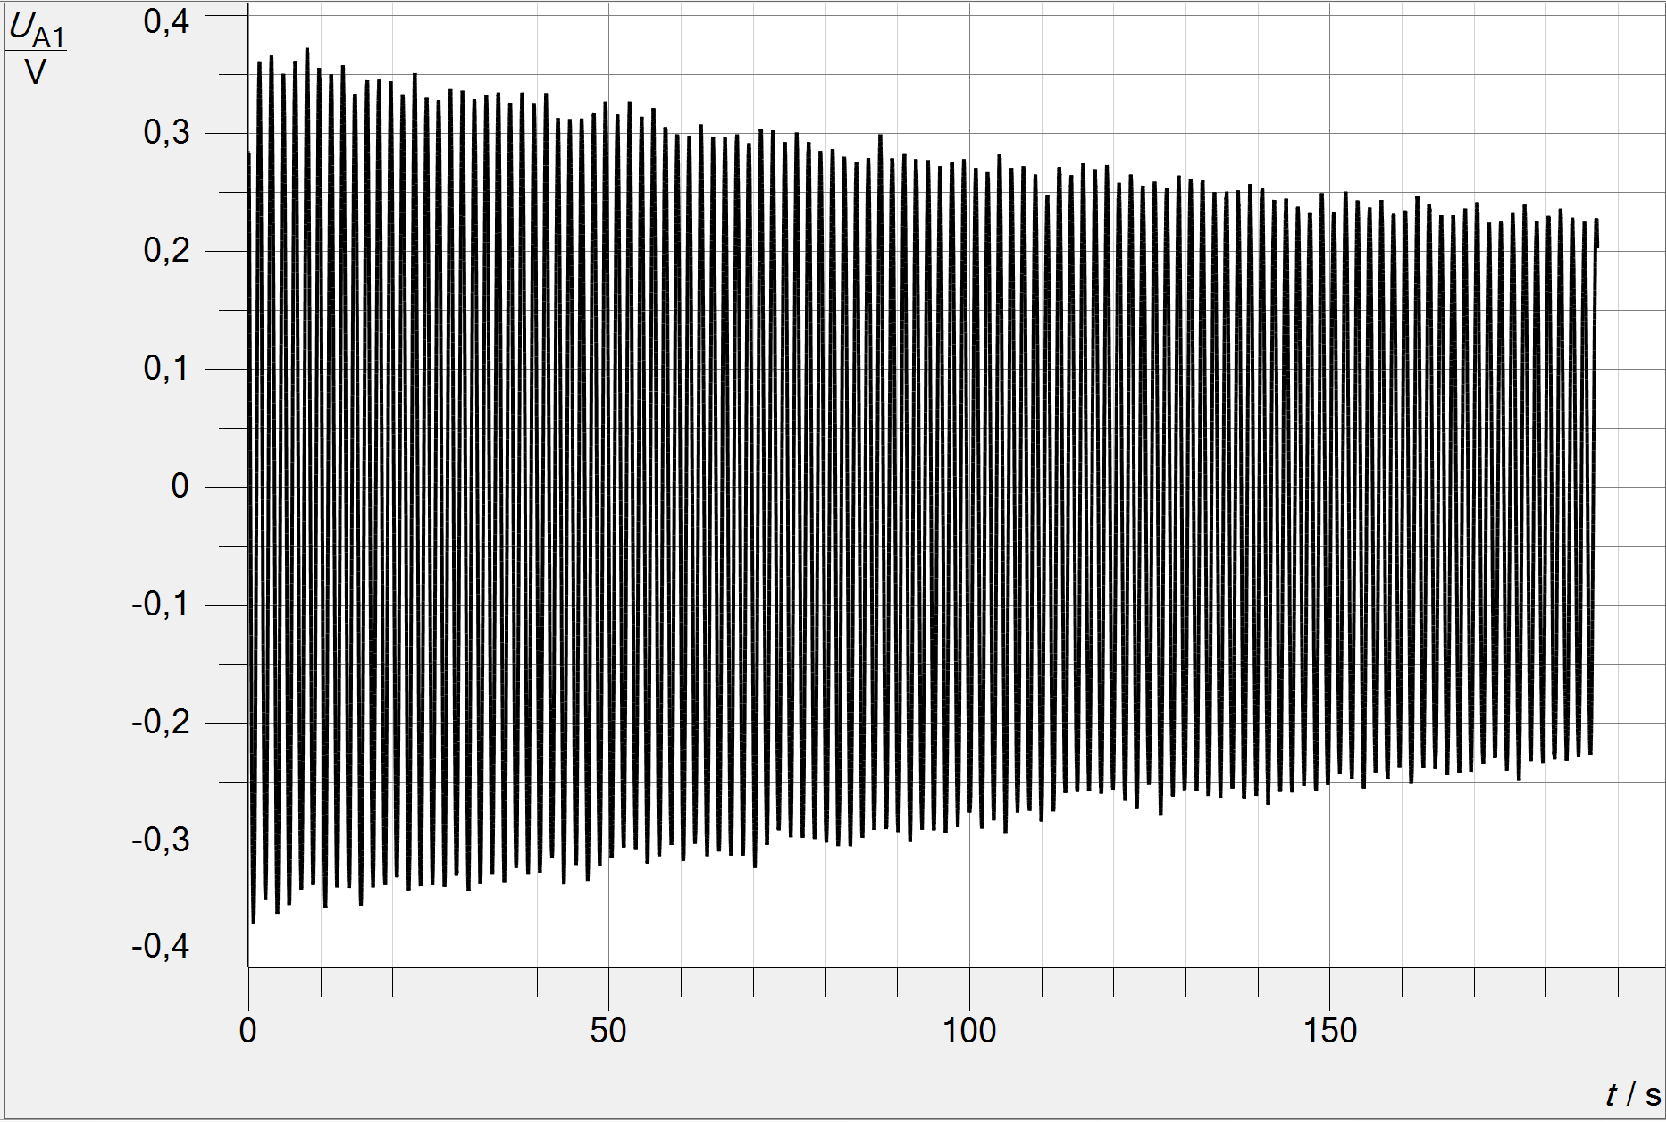
\includegraphics[width=0.9\textwidth]{plots/stange-1-komplett.pdf}
    \caption{Gesamtschwingungsverlauf der ersten Messung ohne Pendelkörper}
\end{figure}
Hier können sie Exemplarisch den Gesamtschwingungsverlauf der ersten Messung sehen bis 185 Sekunden.
Gut zu erkennen ist, dass wir eine Dämpfung der Schwingung haben.
Dies kann man daran sehen, dass die Amplitude der Schwingung mit der Zeit abnimmt. 

Um den genauen Verlauf der Schwingung nach zu volziehen, betrachten wir einen Ausschnitt dieser. 
\begin{figure}[H]
    \centering
    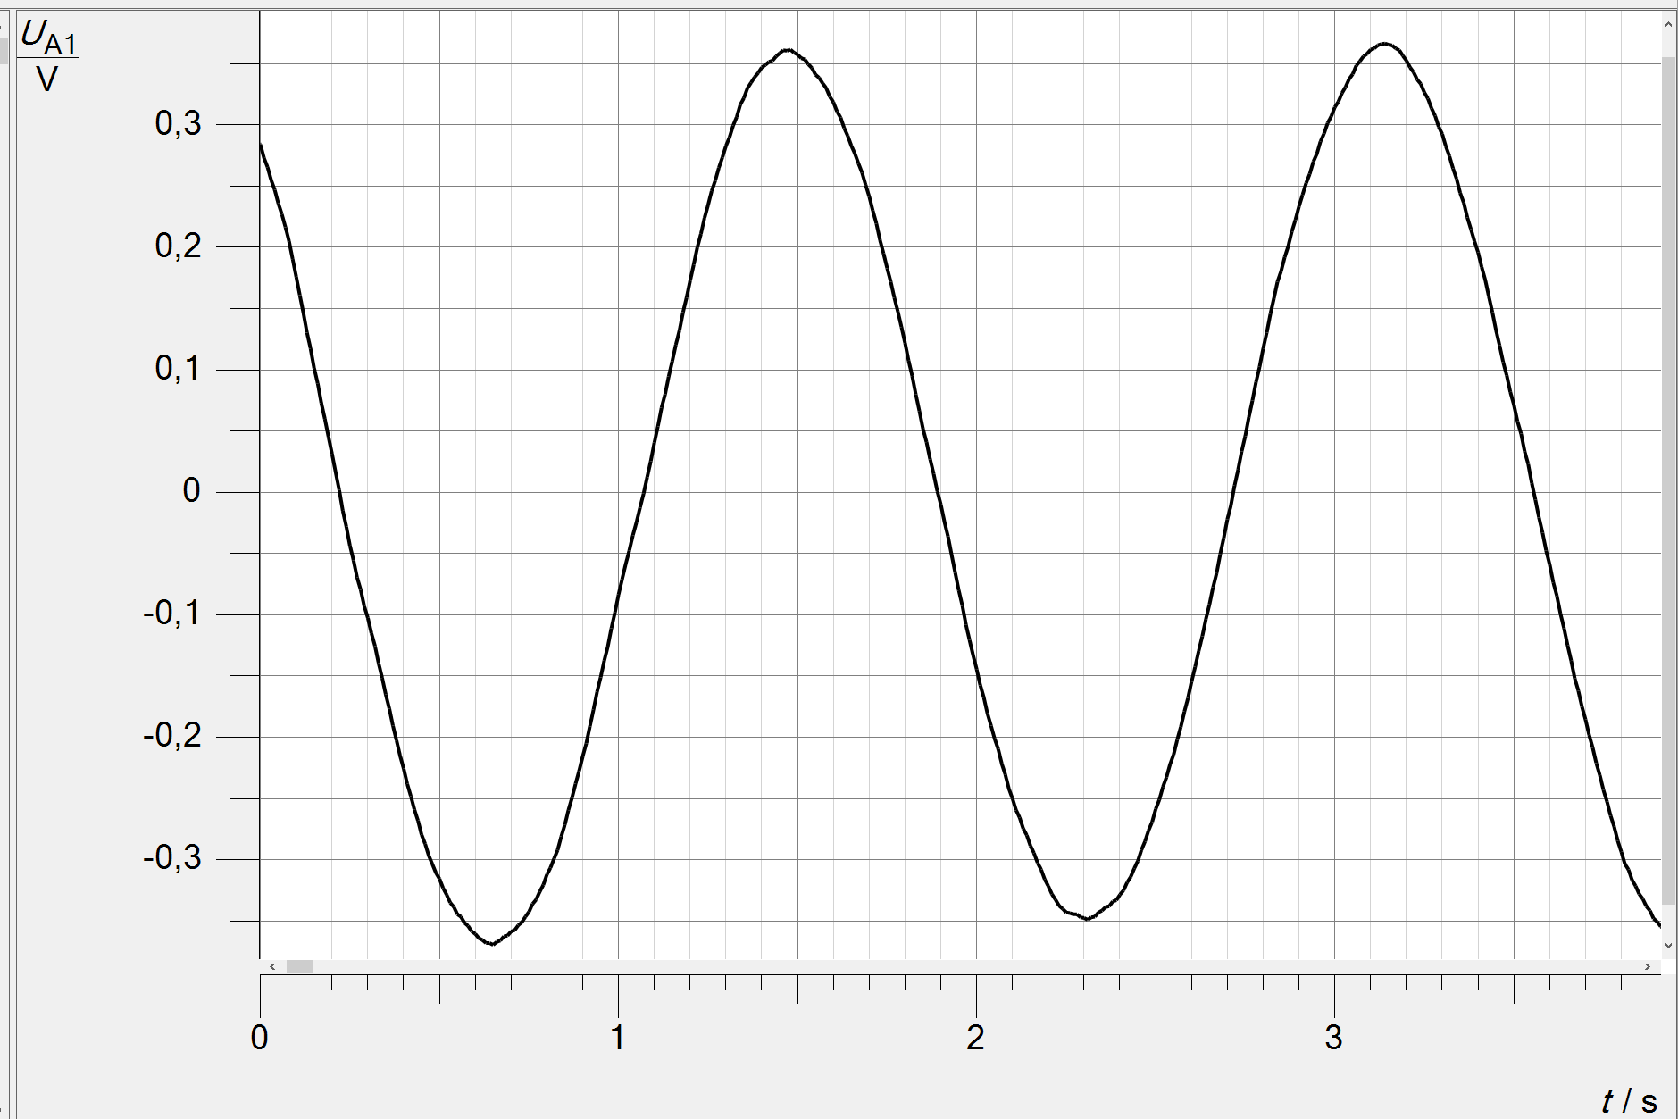
\includegraphics[width=0.7\textwidth]{plots/stange-1-mehrere-schwingungeng.pdf}
    \caption{Ausschnitt des Schwingungsverlauf der ersten Messung ohne Pendelkörper}
\end{figure}

Auf dem Bild sind die ersten 2.25 Schwingungsperioden zu sehen.
Hier können wir gut erkennen, dass die Schwingung einem Kosinus förmigen verlauf hat.  
Sie hat eine Amplitude von ca 0.35 Volt. 
Die in der Graphik angezeigte Nulllinie, wird nicht genau null sein, da es nicht möglich war den Winkelaufnehmer perfekt auf null zu kalibrieren.
Die leichten Unregelmäßigkeiten in der Kurve stammen daher, dass wir nur diskrete Messpunkte haben. 

\begin{figure}[H]
    \centering
    \subfloat{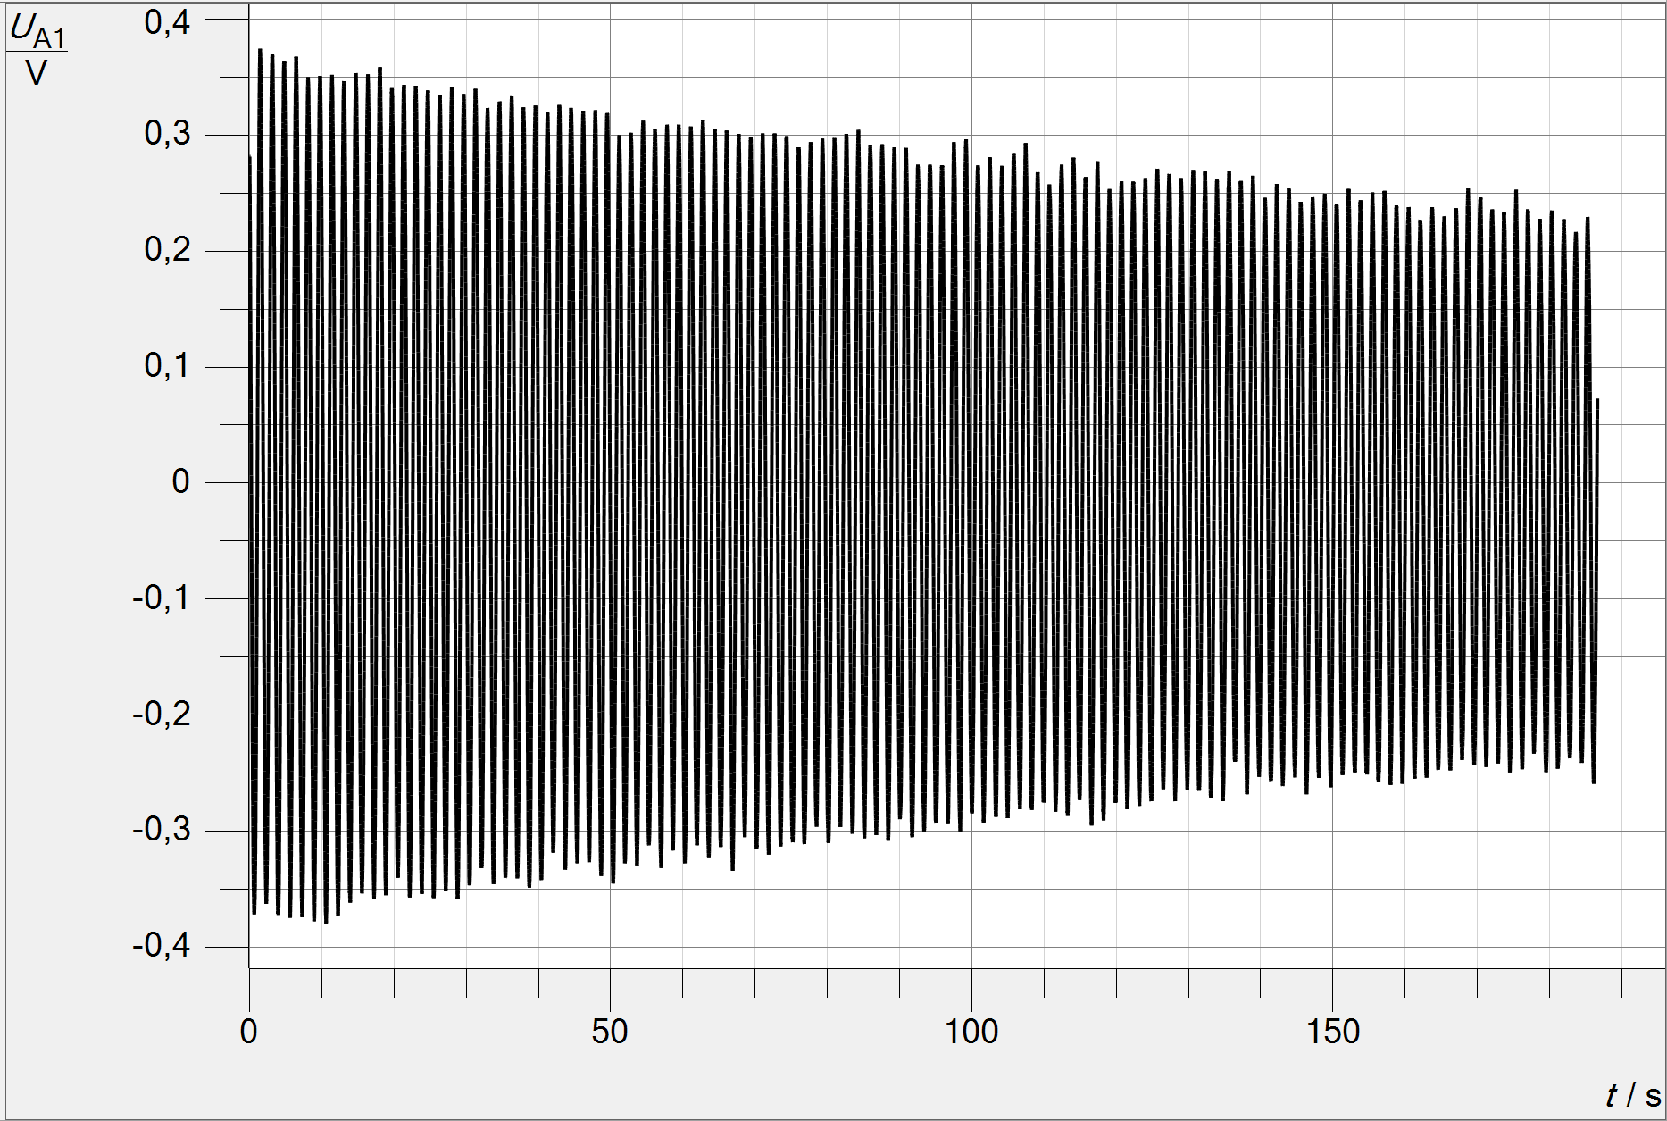
\includegraphics[width=0.45\textwidth]{plots/stange-2-komplett.pdf}}
    \hfill
    \subfloat{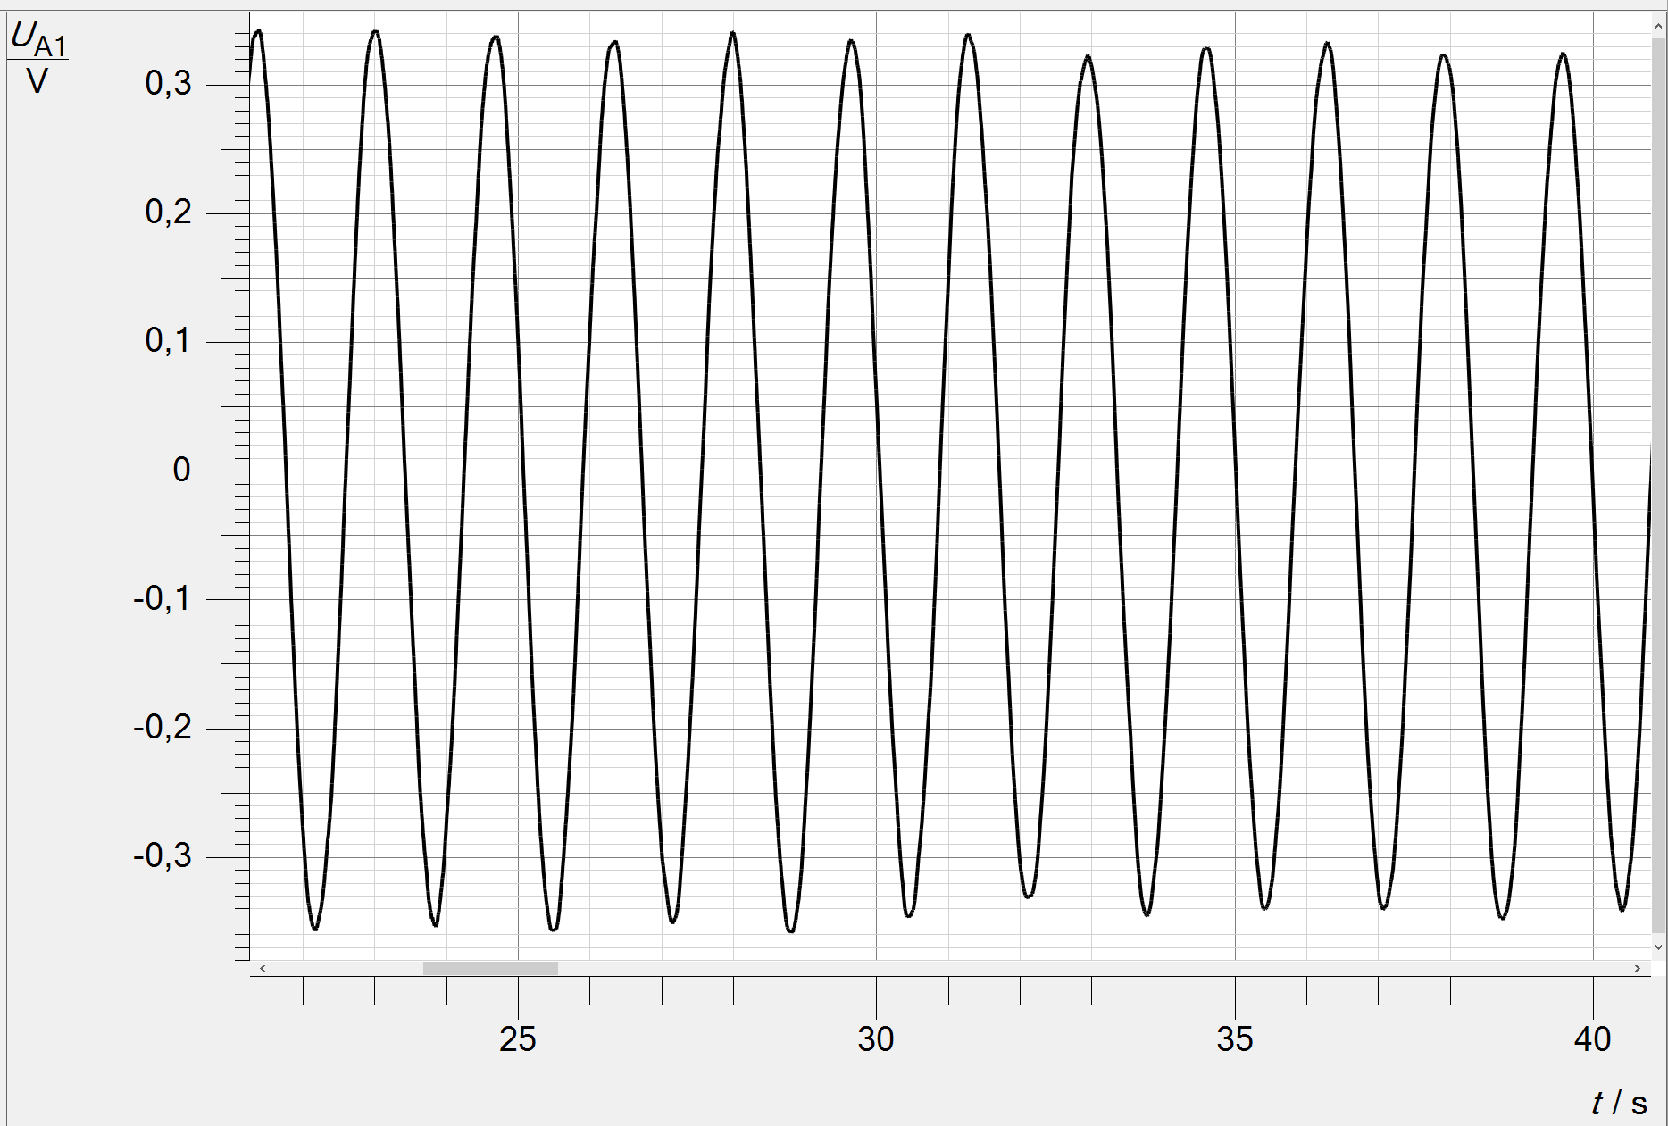
\includegraphics[width=0.45\textwidth]{plots/stange-2-mehrere-schwingungeng.pdf}}
    \caption{Schwingungsverläufe der zweiten Messung ohne Pendelkörper}
\end{figure}

Hier sind die Schwingungsverläufe der zweiten Messung ohne Pendelkörper dargestellt. 
Auch hier können wir die Abnahme der Amplitude sehen.
Hier ist ein größerer Ausschnitt zu sehen. Hier kann man erkennen, dass die Schwingung auch Kosinus förmig Verläuft. 
Beim betrachten der Gesamten Schwingung in CASSY konnten wir sehen, dass dieser Kosinus förmige Verlauf die gesamte Messung über beibehalten wird.
Dies stimmt auch mit den Theoretischen Erwartungen überein.

\begin{figure}[H]
    \centering
    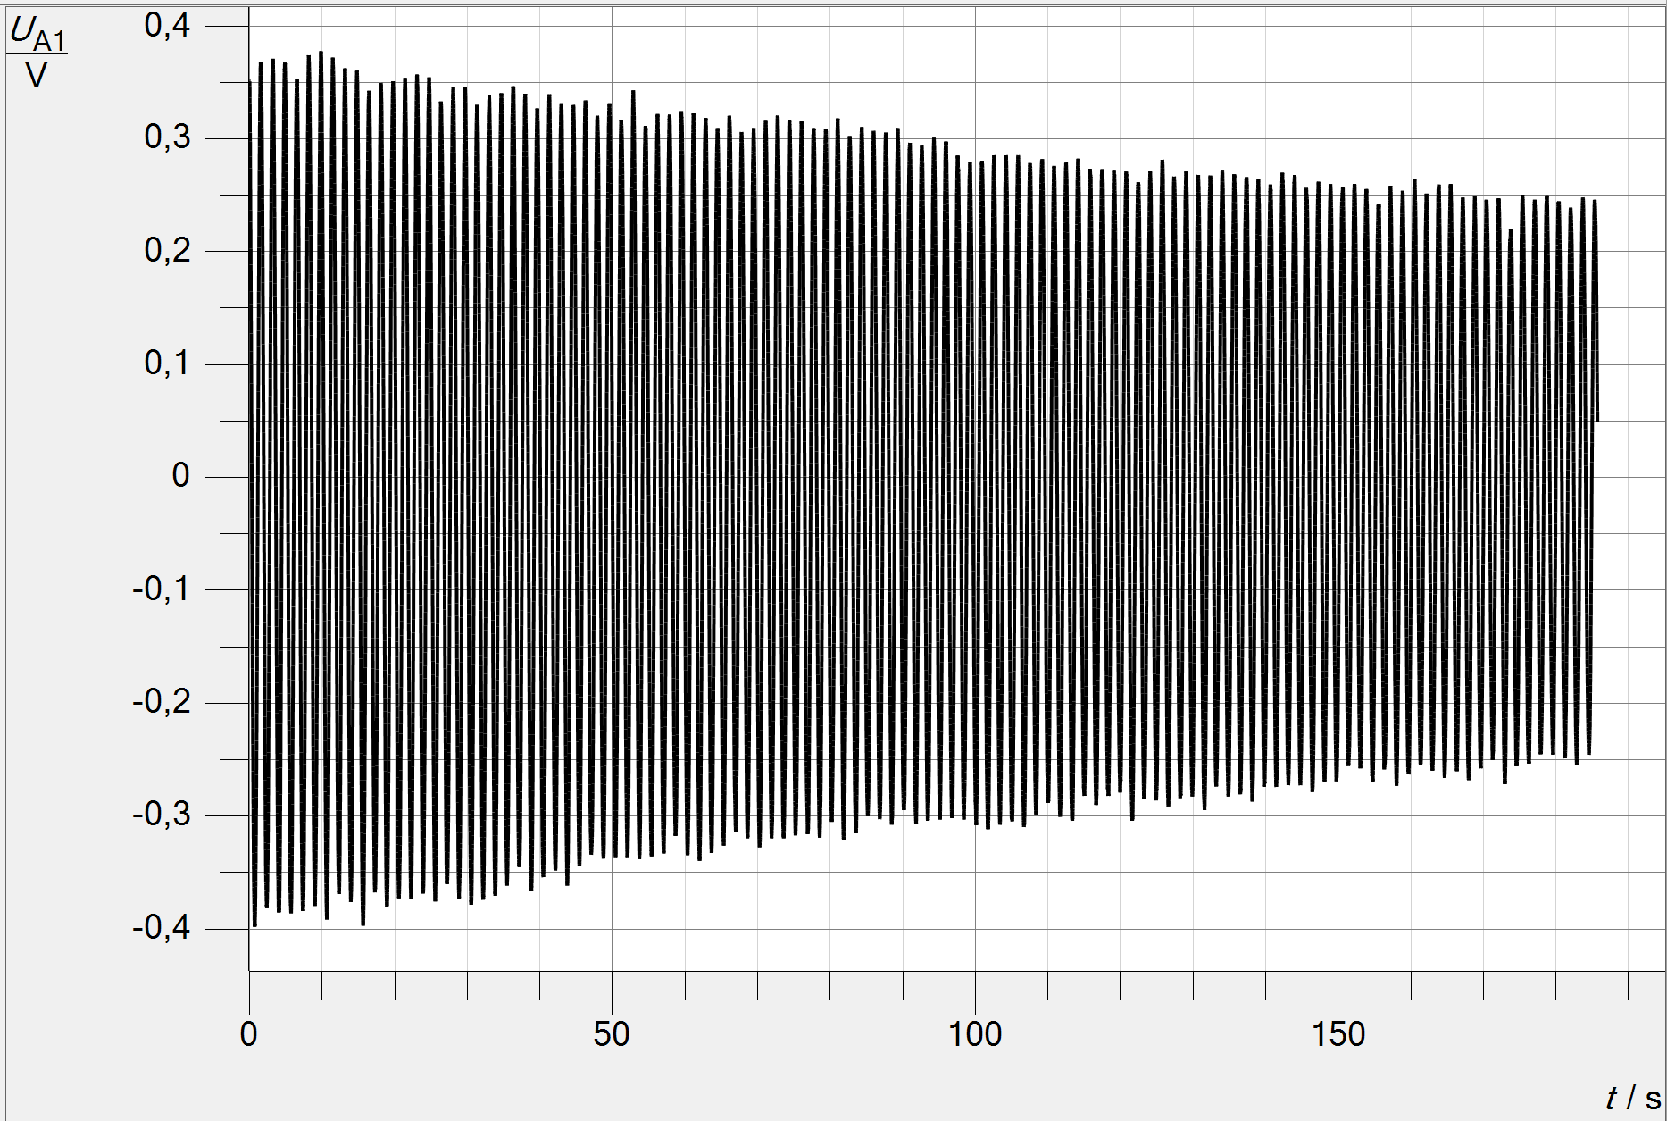
\includegraphics[width=0.7\textwidth]{plots/stange-3-komplett.pdf}
    \caption{Schwingungsverlauf der dritten Messung ohne Pendelkörper}
\end{figure}
\begin{figure}[H]
    \centering
    \subfloat{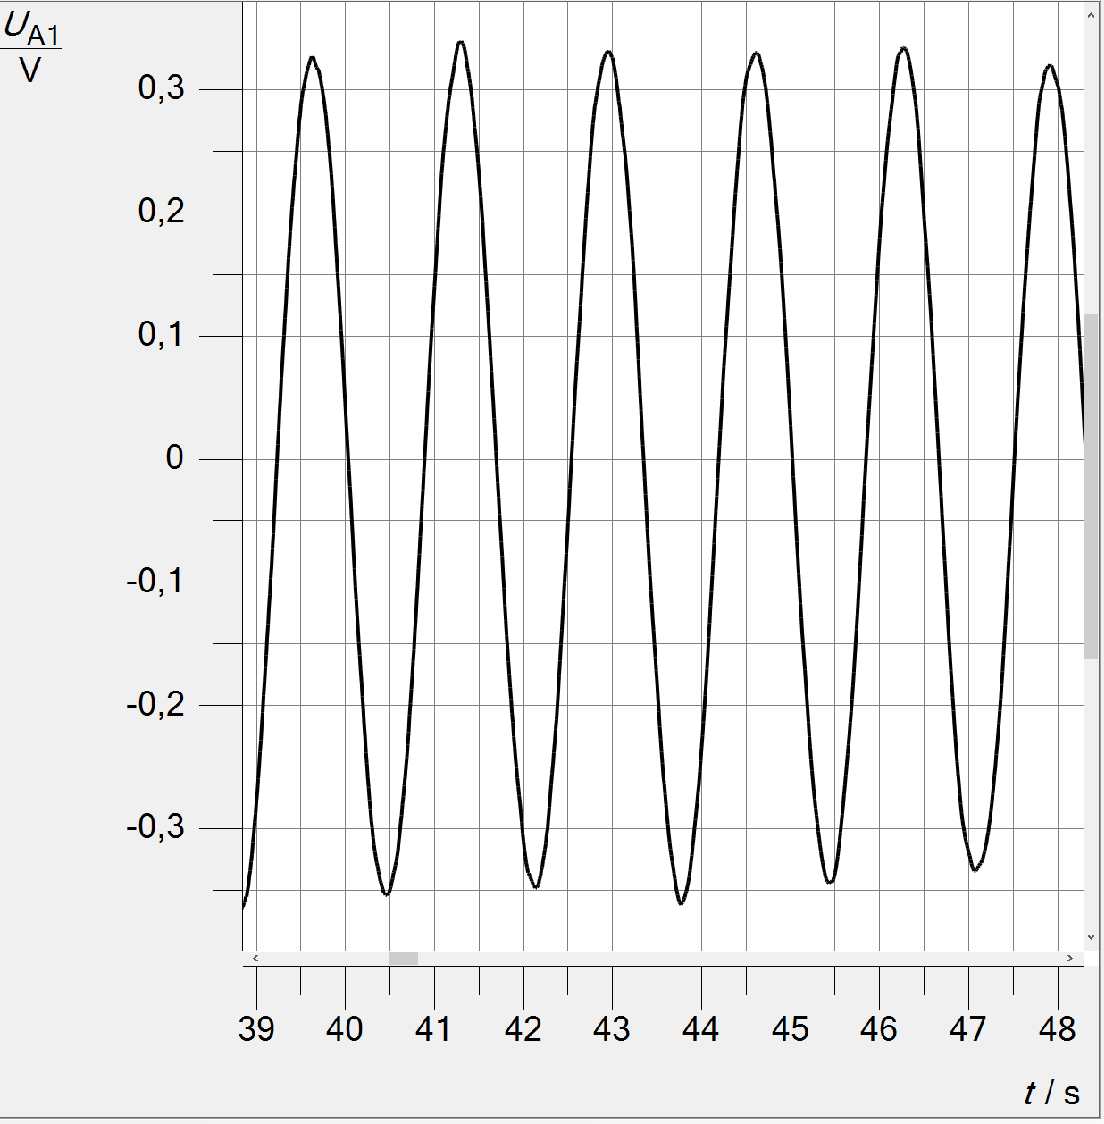
\includegraphics[width=0.45\textwidth]{plots/stange-3-mehrere-schwingungeng.pdf}}
    \hfill
    \subfloat{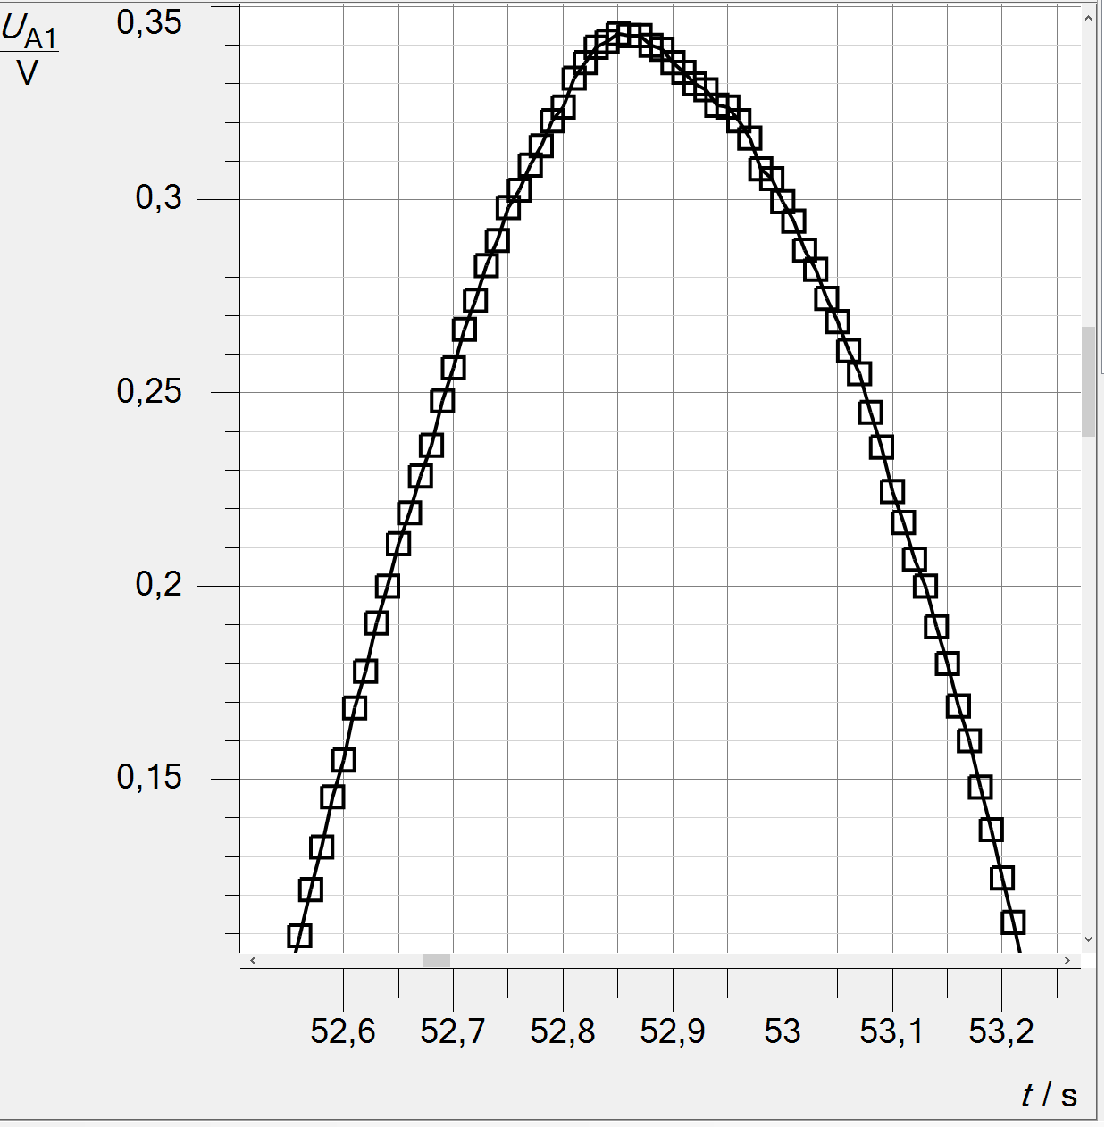
\includegraphics[width=0.45\textwidth]{plots/stange-3-maximum.pdf}}
    \caption{Ausschnitt des Schwingungsverlauf der dritten Messung ohne Pendelkörper}
\end{figure}

Hier sind die Schwingungsverläufe der dritten Messung dargestellt. Diese weisen die selbe Charakteristik auf wie die vorherigen.
Dieses Bild zeigt exemplarisch ein Maxima der Schwingung mit eingezeichneten Datenpunkten. 
Gut zu sehen ist, dass wir diskrete Datenpunkte haben, es liegen genug Datenpunkte im Bereich des Maximums um mit diesen das Maximum zu bestimmen.\\
Während den Messungen haben wir damit wir die Periodendauer überschlagen können, bei CASSY mit dem Peakschwerpunkt das erste und das zwanzigste Maximum bestimmt.

Sobald das Pendel mit Pendelkörper synchronisiert war zu dem ohne Pendelkörper haben wir hier auch drei Messungen durchgeführt.
\begin{figure}[H]
    \centering
    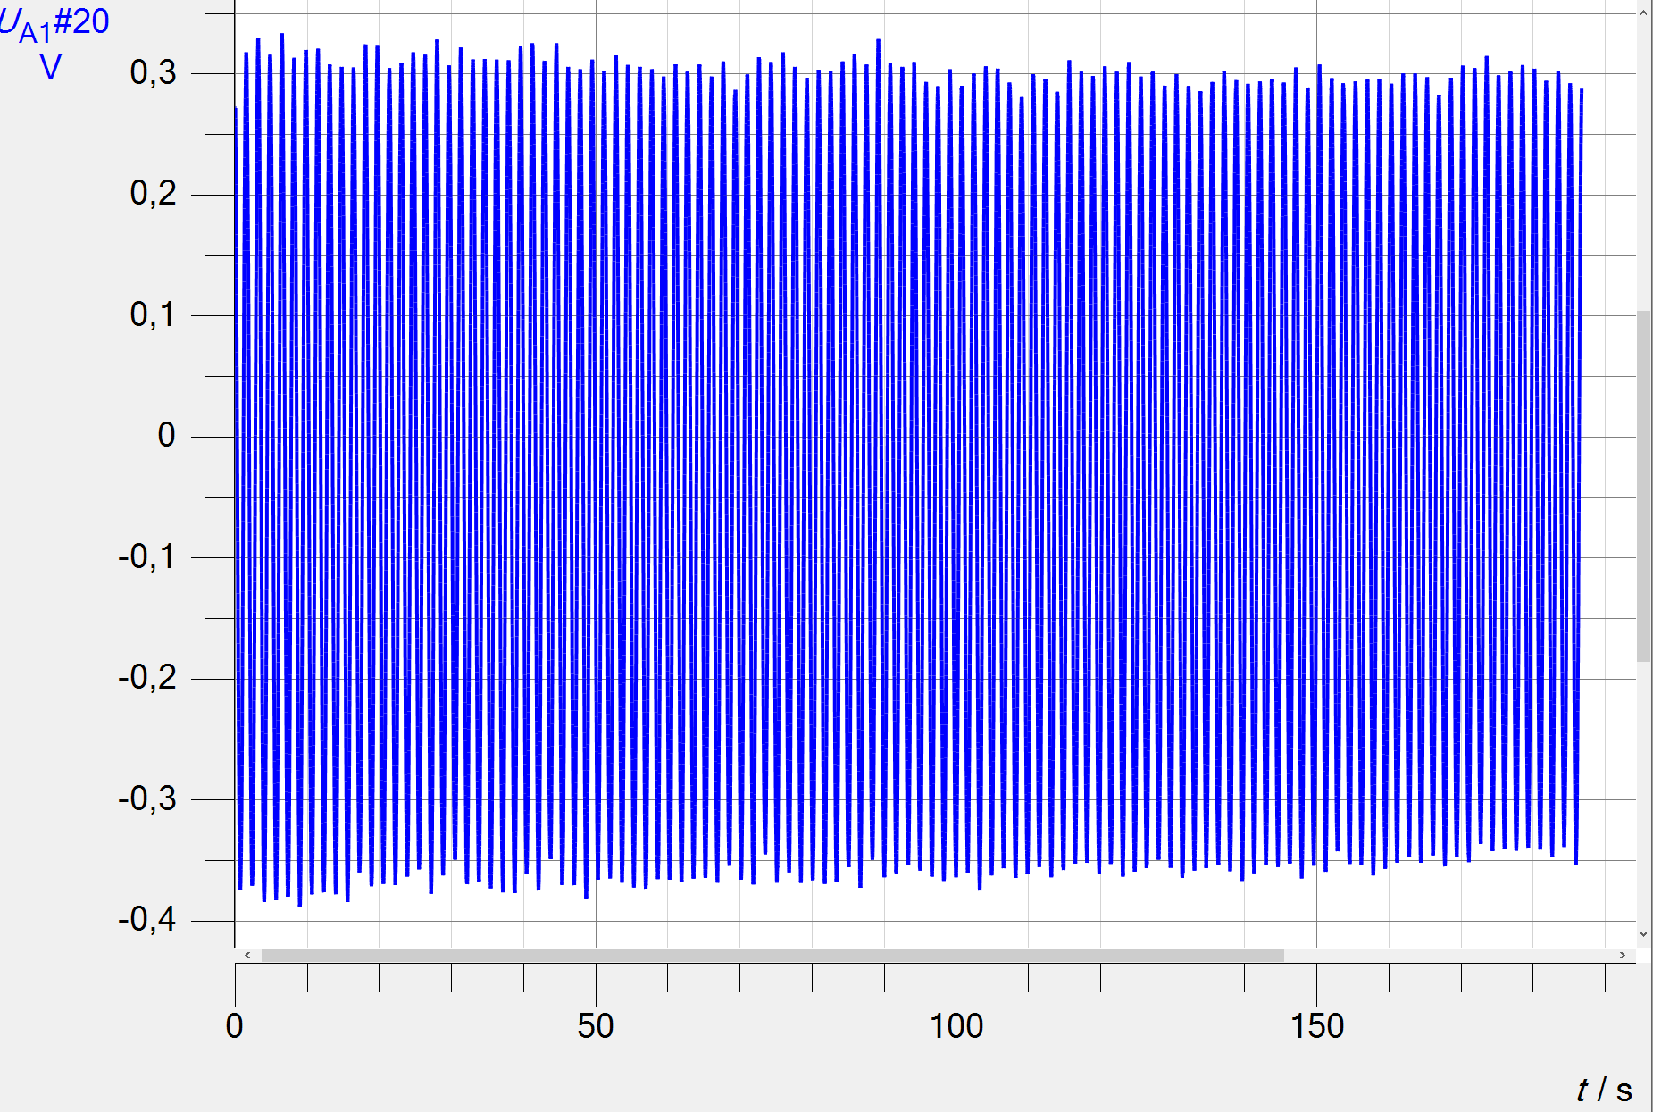
\includegraphics[width=0.9\textwidth]{plots/gewicht-1-komplett.pdf}
    \caption{Schwingungsverlauf der ersten Messung mit Pendelkörper}
    \end{figure}

In diesem Graphen kann man erkennen, dass im Gegensatz, zu dem Schwingvorgang ohne Pendelkörper, die Amplitude der Schwingung kaum abnimmt.
Die Dämpfung ist nach 185s kaum zu erkennen.
Die Amplitude der Maxima schwankt leicht, dies ist in allen Schwingungsverläufen mit und ohne Pendelkörper zu sehen.\\

Die zwei Hauptfaktoren der Dämpfung sind der Luftwiederstand und die Reibung am Auflagepunkt der Nadel. 
Da wir kaum Amplitudenabnahme mit Pendelkörper feststellen können, können wir daraus schließen, dass der Luftwiederstand den größeren Anteil der Dämpfung liefert.

\begin{figure}[H]
    \centering
    \subfloat{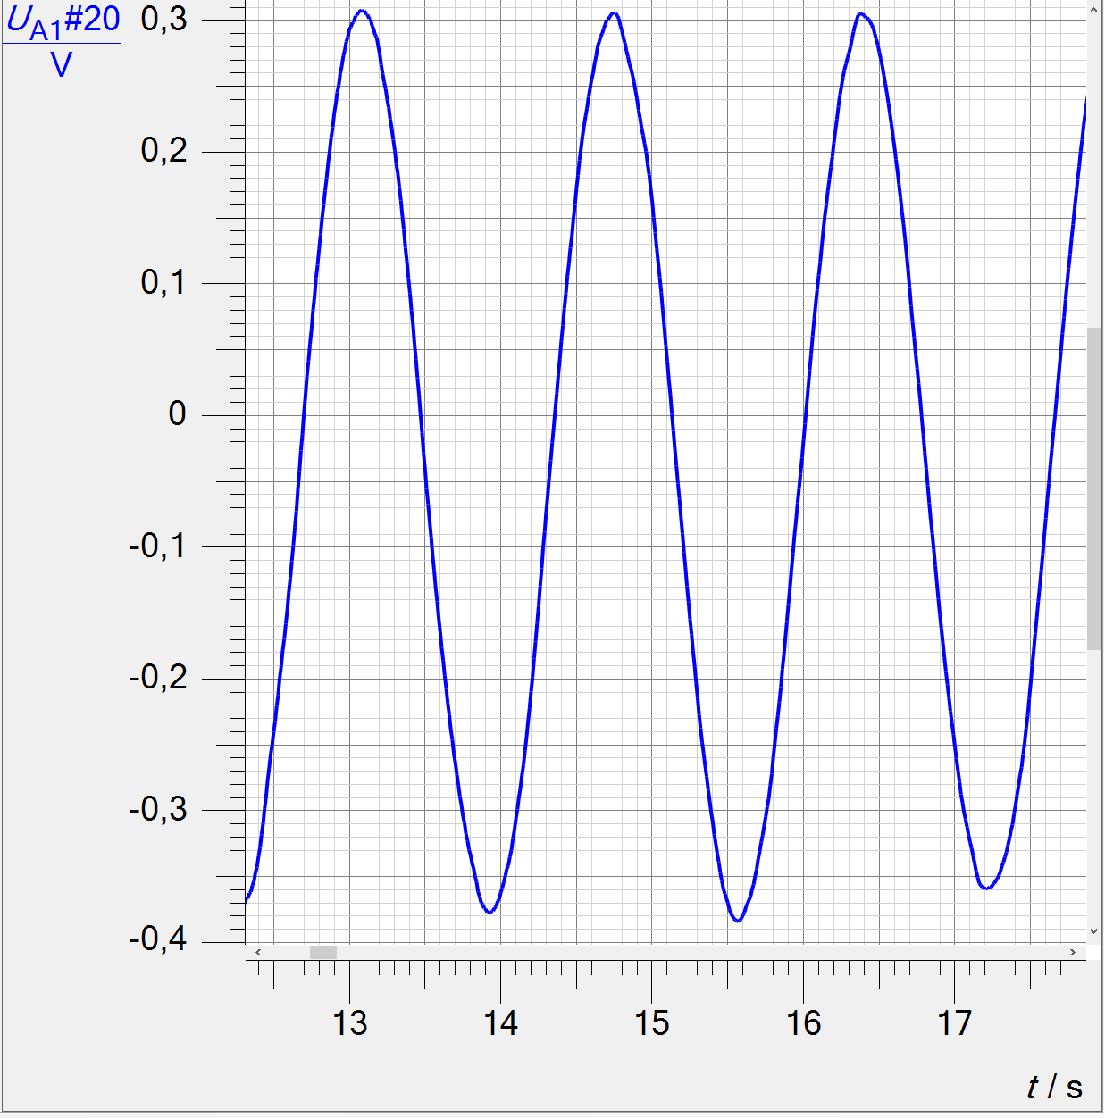
\includegraphics[width=0.4\textwidth]{plots/gewicht-1-mehrere-schwingungen.pdf}}
    \hfill
    \subfloat{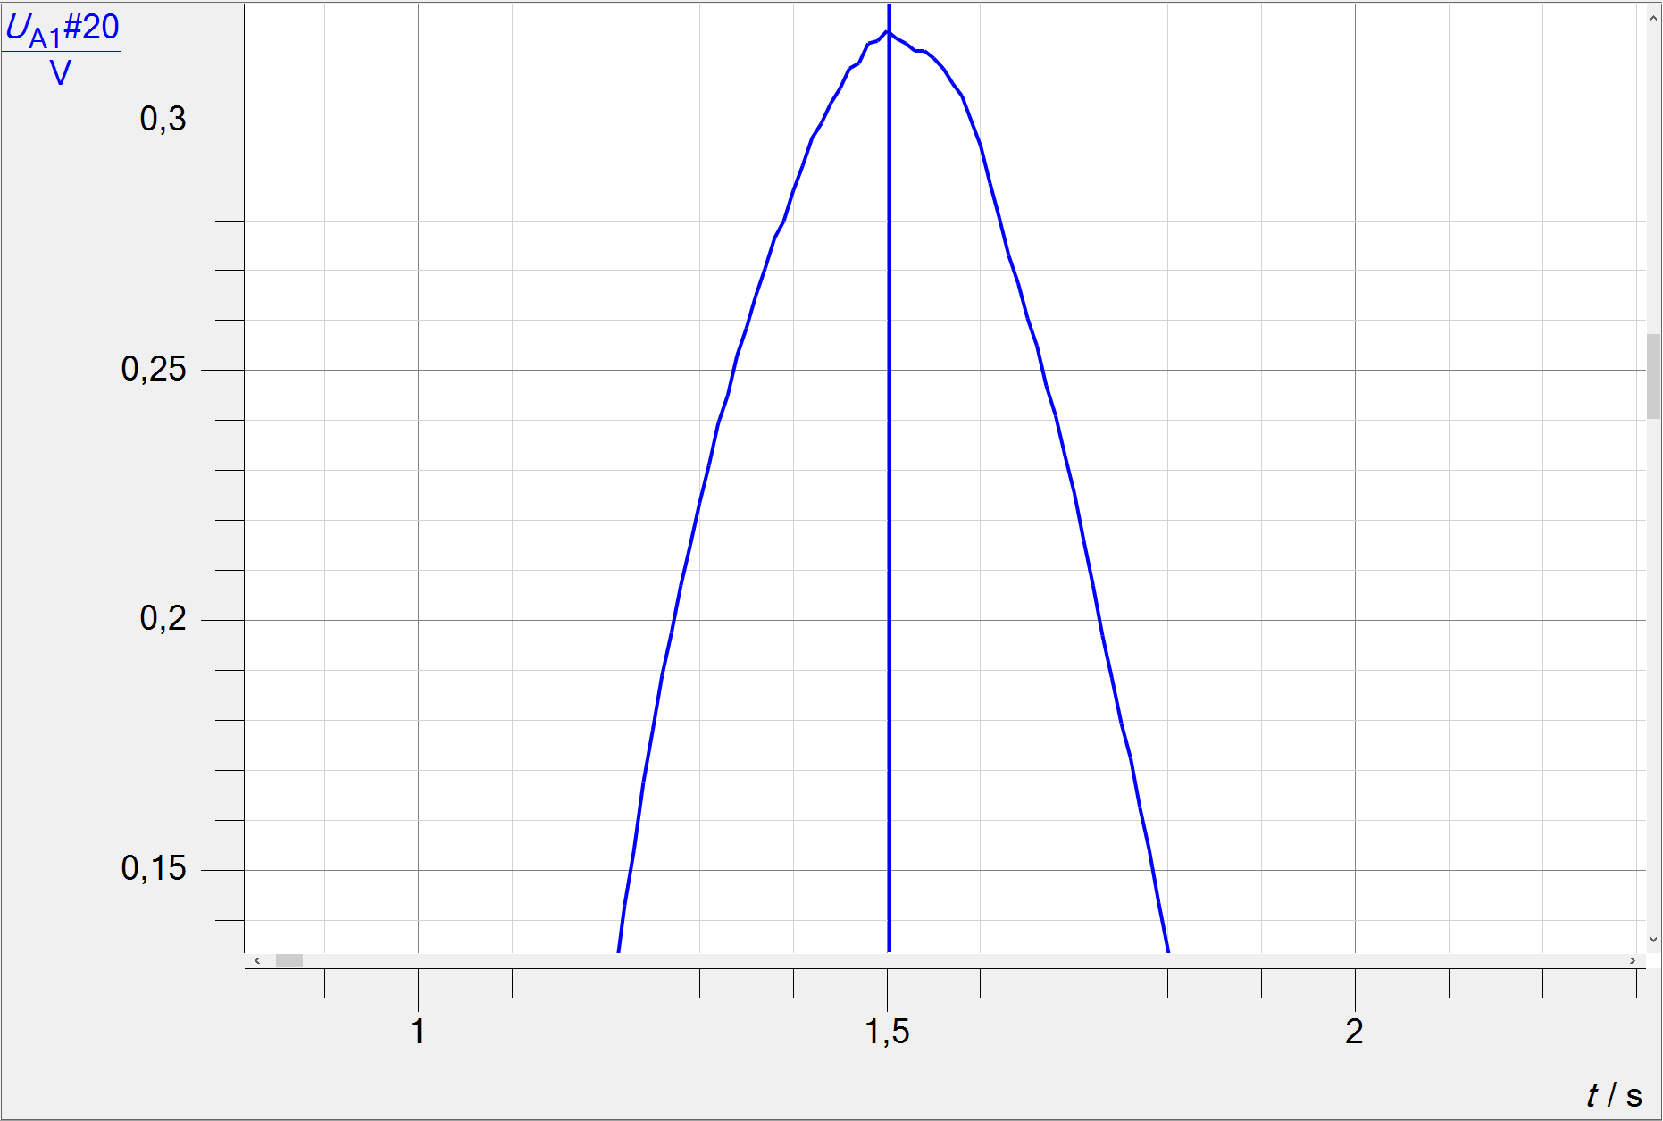
\includegraphics[width=0.55\textwidth]{plots/gewicht-1-peak-schnell.pdf}}
    \caption{Ausschnitt des Schwingungsverlauf der ersten Messung mit Pendelkörper}
    \end{figure}

Auch hier können wir erkennen, dass die Schwingung einem Kosinus förmigen Verlauf folgt.
Zum Vergleich der Periodendauern haben wir wieder das erste und das zwanzigste Maximum bestimmt.
Exemplarisch ist hier das Ablesen des ersten Maximums dargestellt.

Für die Weiteren Messungen sind hier auch die Schwingungsverläufe Dargestellt.
Für jede Messung der komplette Schwingungsverlauf und ein Ausschnitt der Schwingung. 

\begin{figure}[H]
    \centering
    \subfloat{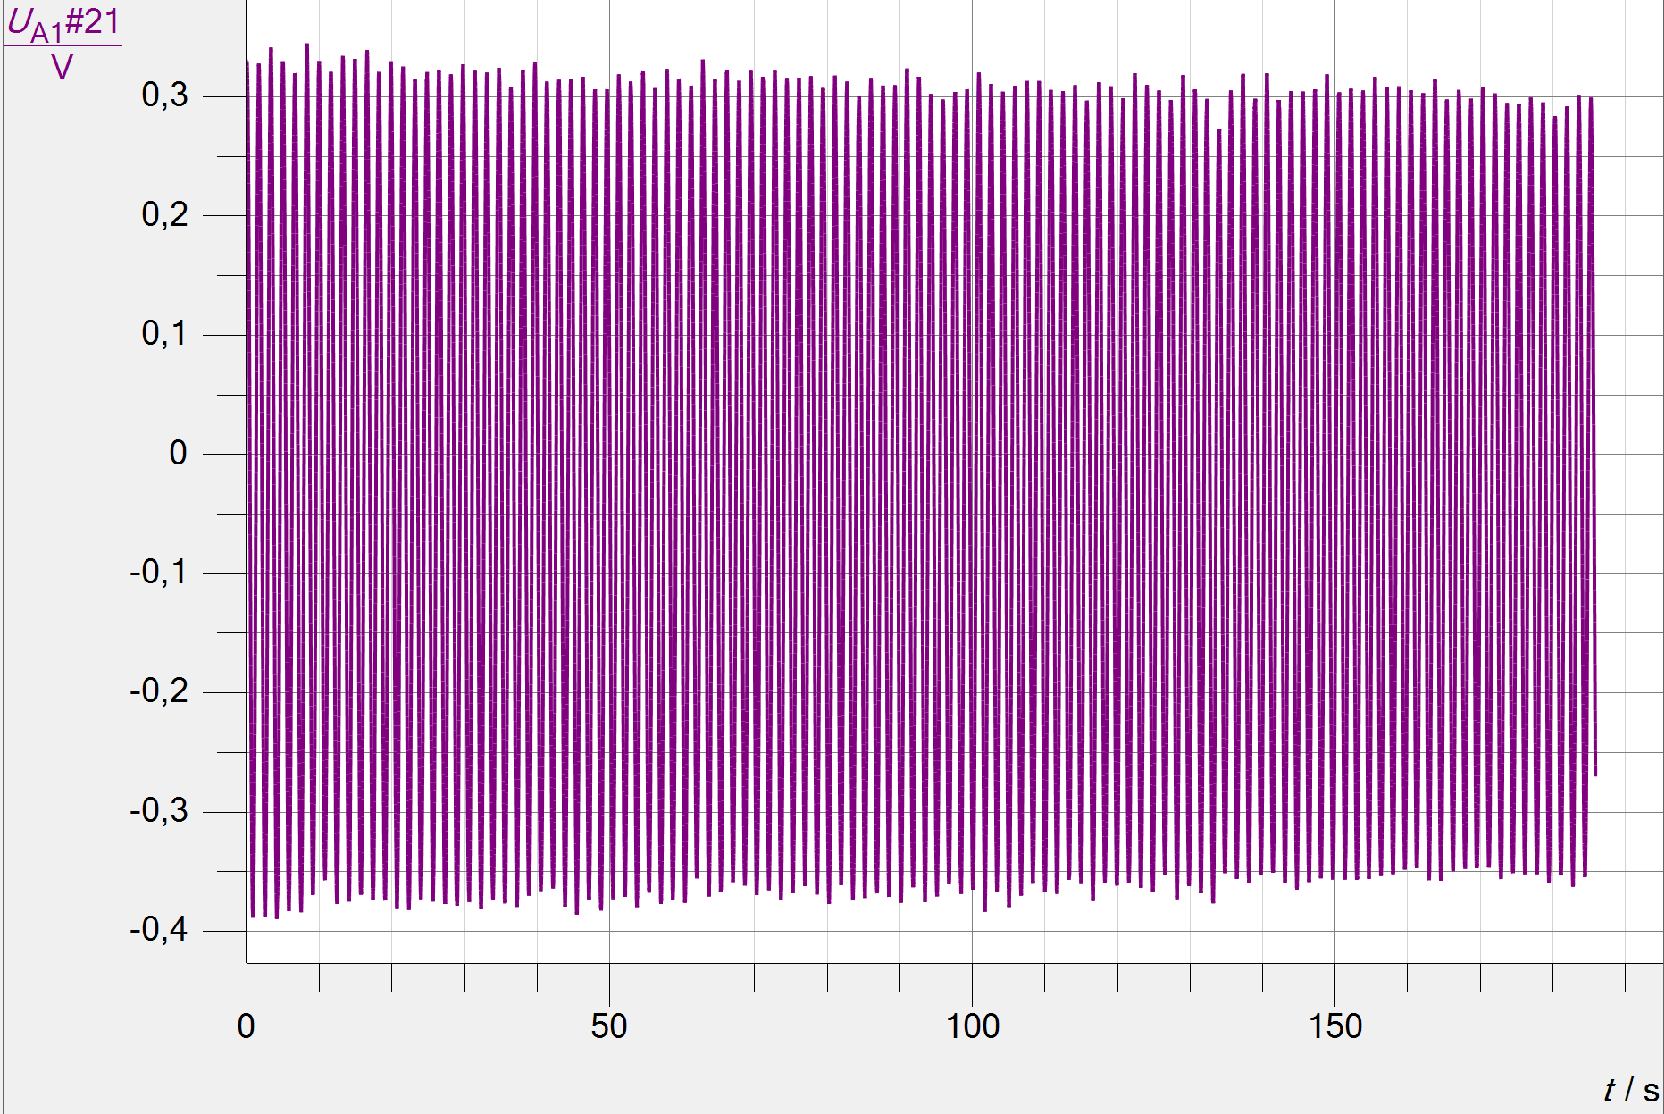
\includegraphics[width=0.55\textwidth]{plots/gewicht-2-komplett.pdf}}
    \hfill
    \subfloat{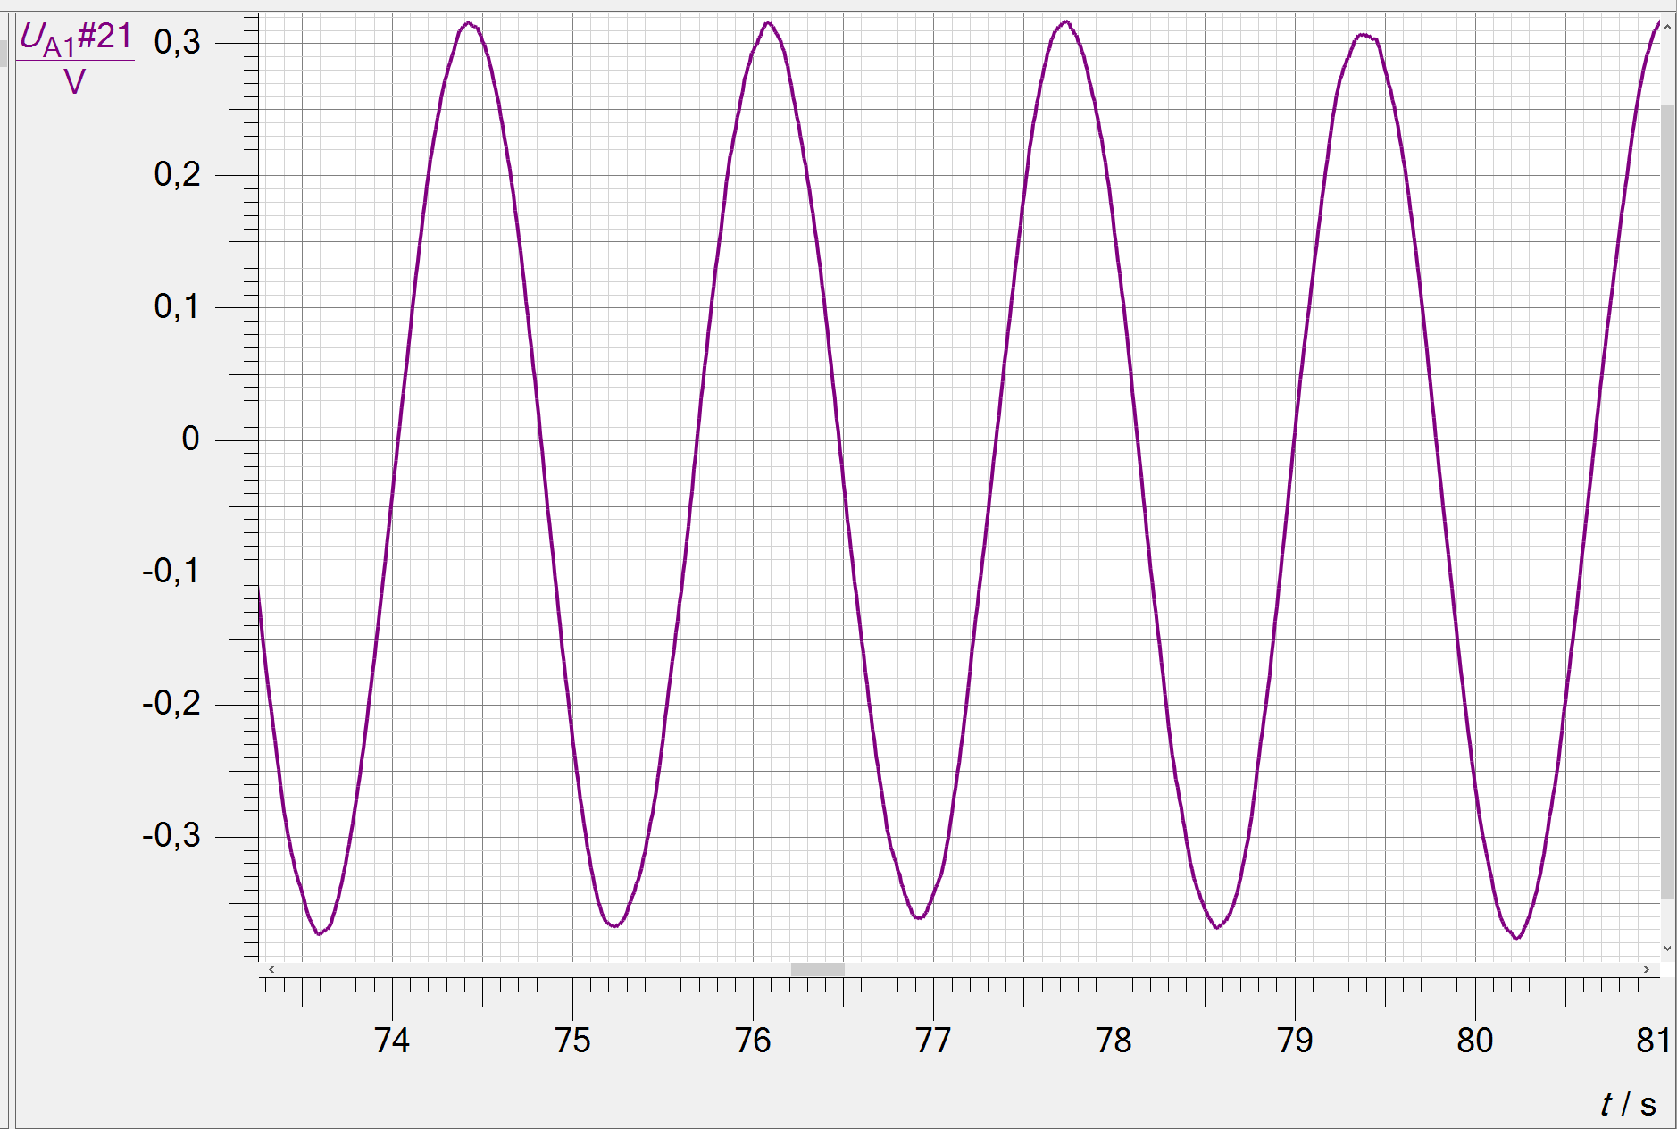
\includegraphics[width=0.40\textwidth]{plots/gewicht-2-schwungungen.pdf}}
    \caption{Schwingungsverlauf der zweiten Messung mit Pendelkörper}
    \end{figure}
 
\begin{figure}[H]
    \centering
    \subfloat{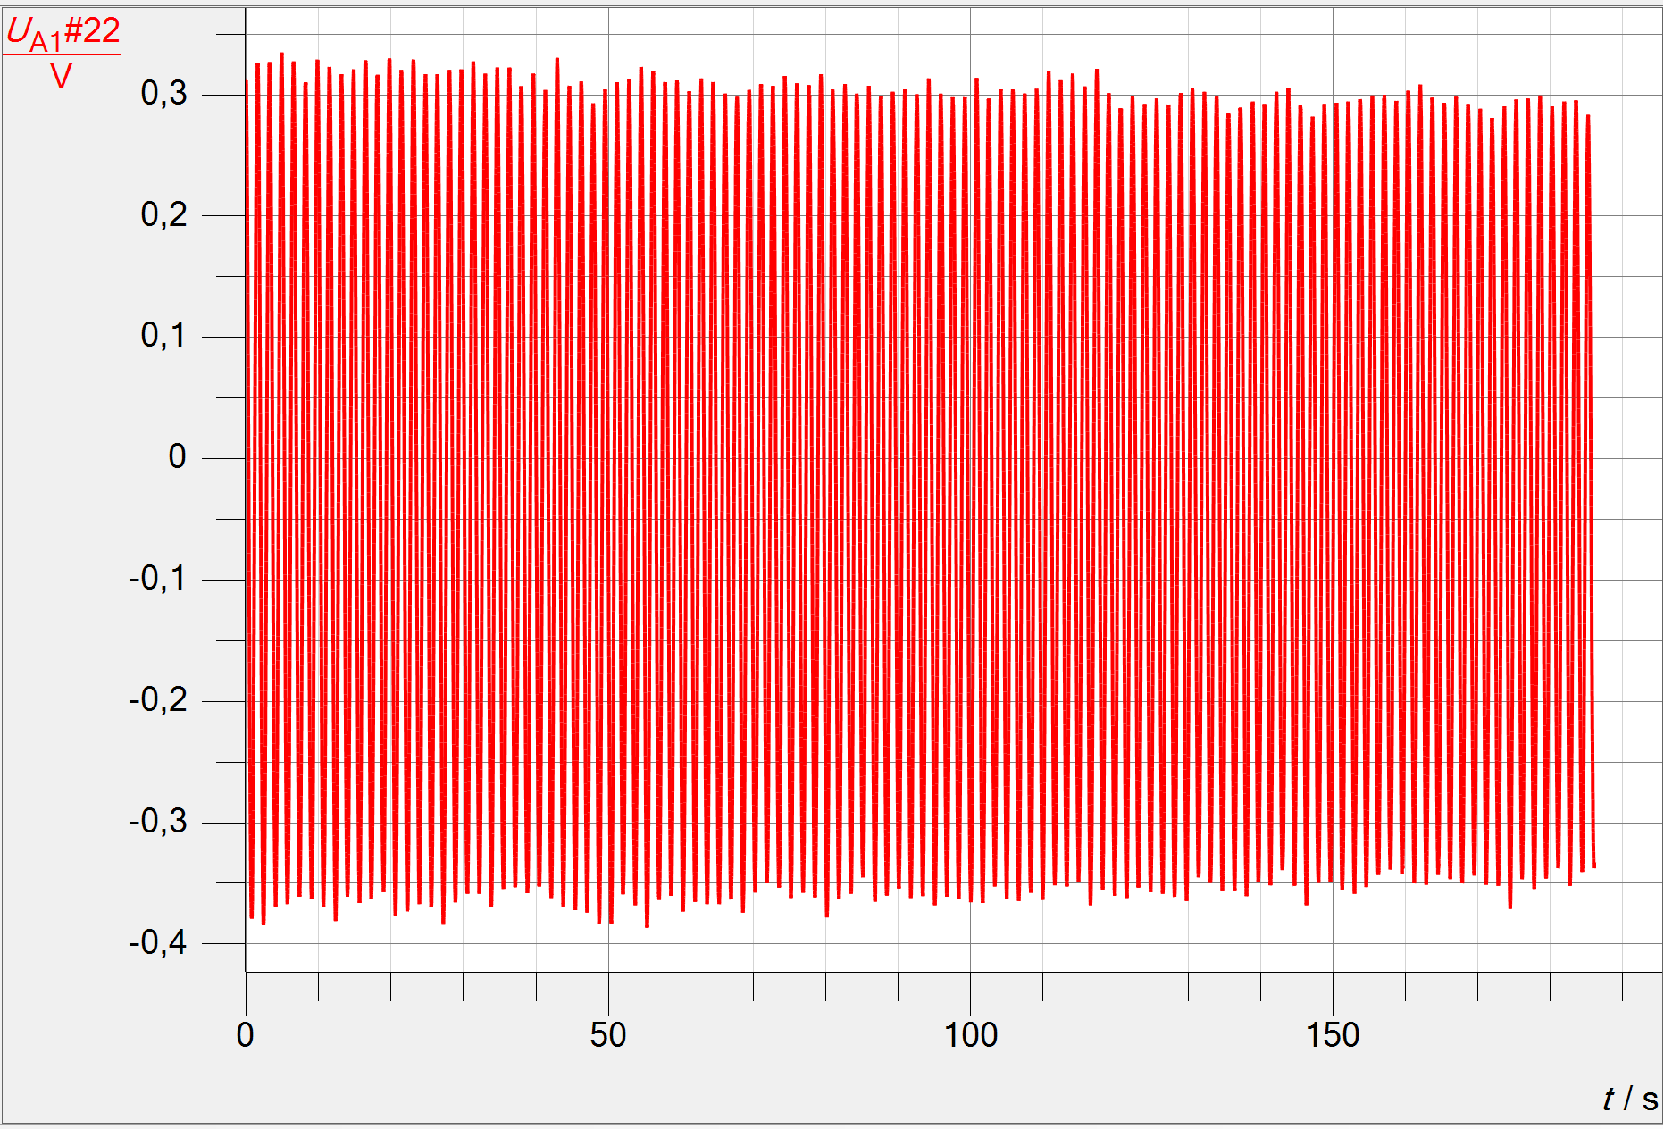
\includegraphics[width=0.55\textwidth]{plots/gewicht-3-komplett.pdf}}
    \hfill
    \subfloat{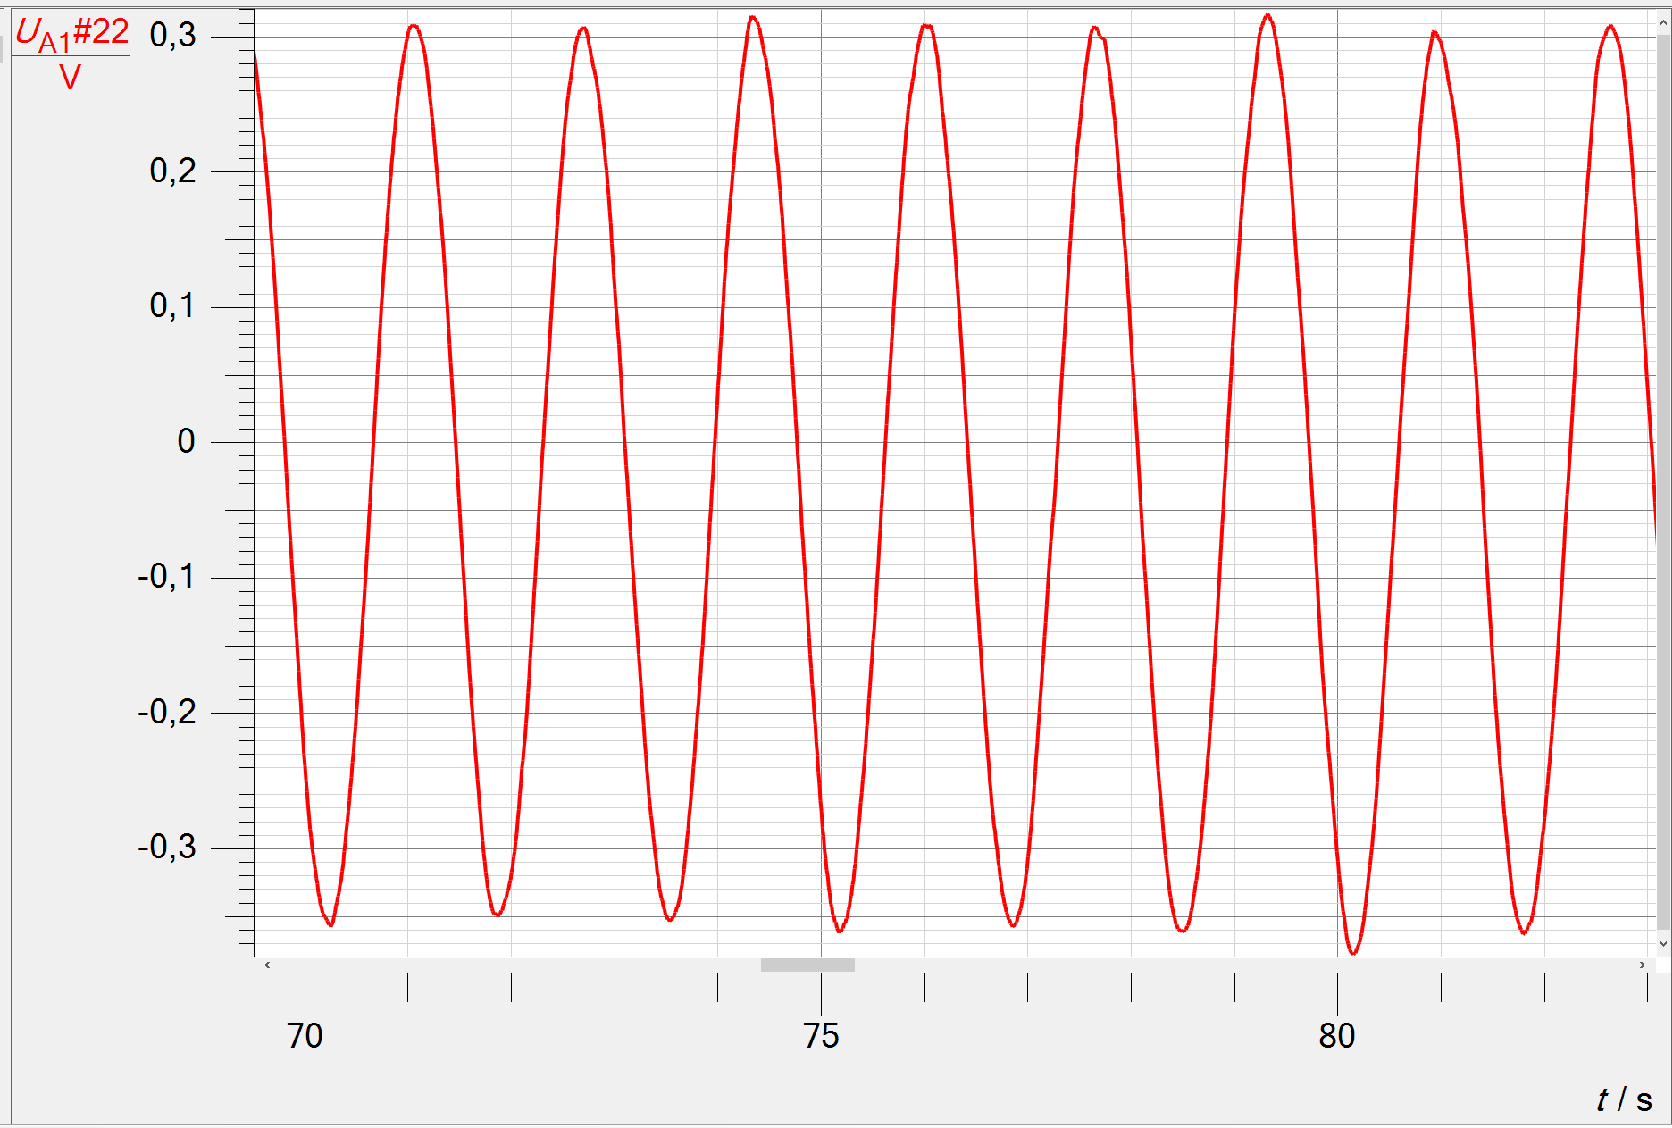
\includegraphics[width=0.40\textwidth]{plots/gewicht-3-schwungungen.pdf}}
    \caption{Schwingungsverlauf der dritten Messung mit Pendelkörper}
    \end{figure}

Zuletzt ist hier noch eine Nahaufnahme eines Maxima gezeigt, in dieser kann man erkennen, dass die Messpunkte um das Maxima nicht perfekt Kosinus förmig sind.
Dies ist jedoch zur Bestimmung des Peaks kein problem, da wir hierfür den Peakschwerpunkt berechnen.

\begin{figure}[H]
    \centering
    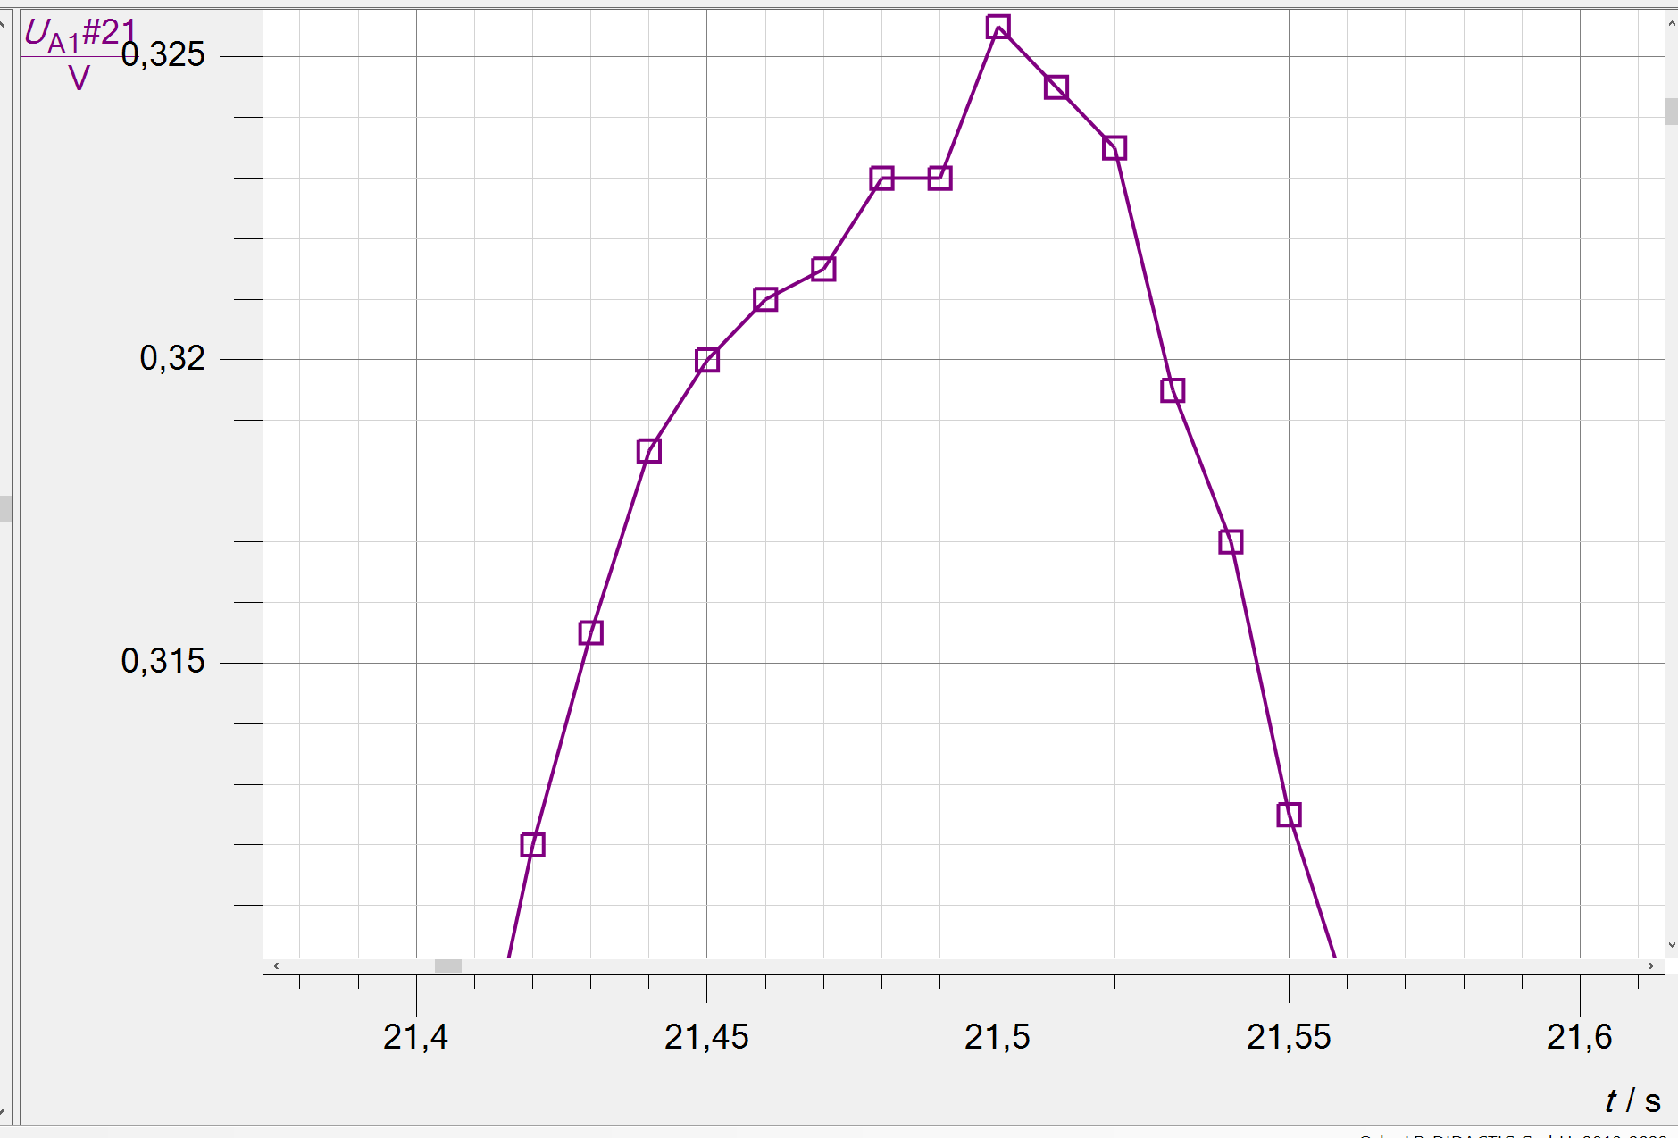
\includegraphics[width=0.6\textwidth]{plots/gewicht-2-peak.pdf}
    \caption{Peak der zweiten Messung mit Pendelkörper}
    \end{figure}
     
     
\begin{aufgabe}{Auswertung}
  Bestimmen Sie für alle Messreihen die Periodendauer und ihre
  Messunsicherheit, indem Sie eine geeignete lineare Regression
  durchführen. Demonstrieren Sie, dass Sie das Trägheitsmoment der
  Stange kompensiert haben. Tabellieren Sie die Zwischenergebnisse
  der relevanten Größen samt ihrer Messunsicherheiten. Berechnen
  Sie die Erdbeschleunigung. Führen Sie eine Fehlerrechnung zur
  Bestimmung der Messunsicherheit durch. Geben Sie bei Ihrer
  Fehlerrechnung die Größe der Einzelbeiträge an, die zu dem
  Gesamtfehler führen. Diskutieren Sie, welcher Fehler den
  Gesamtfehler dominiert. Vergleichen Sie Ihr Endergebnis mit dem
  relevanten Literaturwert.
\end{aufgabe}
\section{Auswertung}

\subsection{Unsicherheiten auf den Abgelesenen Zeitpunkte}
Allgemein unterscheidet man zwischen systematischen und statistischen Fehlern.
Bei der Zeit haben wir keinen Systematischen Fehler.
Der Statistische Fehler kommt in unserem Falle durch das ablesen.
Um diesen möglichst präzise zu bestimmen, haben wir ihn für jede der 6 Messungen einzeln bestimmt.
Eigentlich sollte der einmal bestimmte Ablesefehler für alle Messungen gelten, da wir immer die gleiche Messmethode und Messeinstellungen hatten, und auch alle Pendel ungefähr mit der gleichen Frequenz geschwungen sind.
Da wir beim anschauen der Rohdaten aber festgestellt haben, das nicht alle Peaks von allen Messreihen gleich sauber sind, haben wir den Fehler für jede Messung einzeln analysiert.
Zudem ist die hier bestimmte Unsicherheit auch wichtig für das Chi-Quadrat, weshalb es für jede Messreihe genau passen sollte.\\
 
 
Wir haben alle Peaks mit der Peakschwerpunkt Methode von Cassy bestimmt.
Diese haben wir benutzt, da wir wissen, das unser Signal einer Sinusfunktion folgt.
Mithilfe der Schwerpunkts Methode wird berücksichtigt, das wenn das Maximum zwischen 2 Punkten liegt, die umliegenden Punkte mit verwendet werden können, um die genaue position des Maximums zu gewichten.
Da es immer mehrere mögliche sinnvolle Grenzen für den Peakschwerpunkt gibt, haben wir hier für die 1. Messung des Pendels ohne Gewicht, die gewählten Grenzen bei der Fehler Bestimmung genau gezeigt.
Dabei haben wir bei der Bestimmung des Ablesefehlers die Grenzen versucht ähnlich zu wählen, wie wir sie auch vorher bei der Bestimmung der Peaks gewählt haben.
Insegasmt haben wir 5 bis 6 verschieden Grenzen genommen. Diese haben wir vom Peak abhängig gemacht. Wir haben darauf geachtet diese nicht immer symmetrisch zu wählen.
Die schwankung der bestimmten peaks haben wir dann statistisch analysiert. 
(Die Reihenfolge der Nummerierung ist nicht die Reihenfolge der Grenzen, sonder dient um das vorgehen zu beschreiben)
\begin{figure}[H]
    \centering
    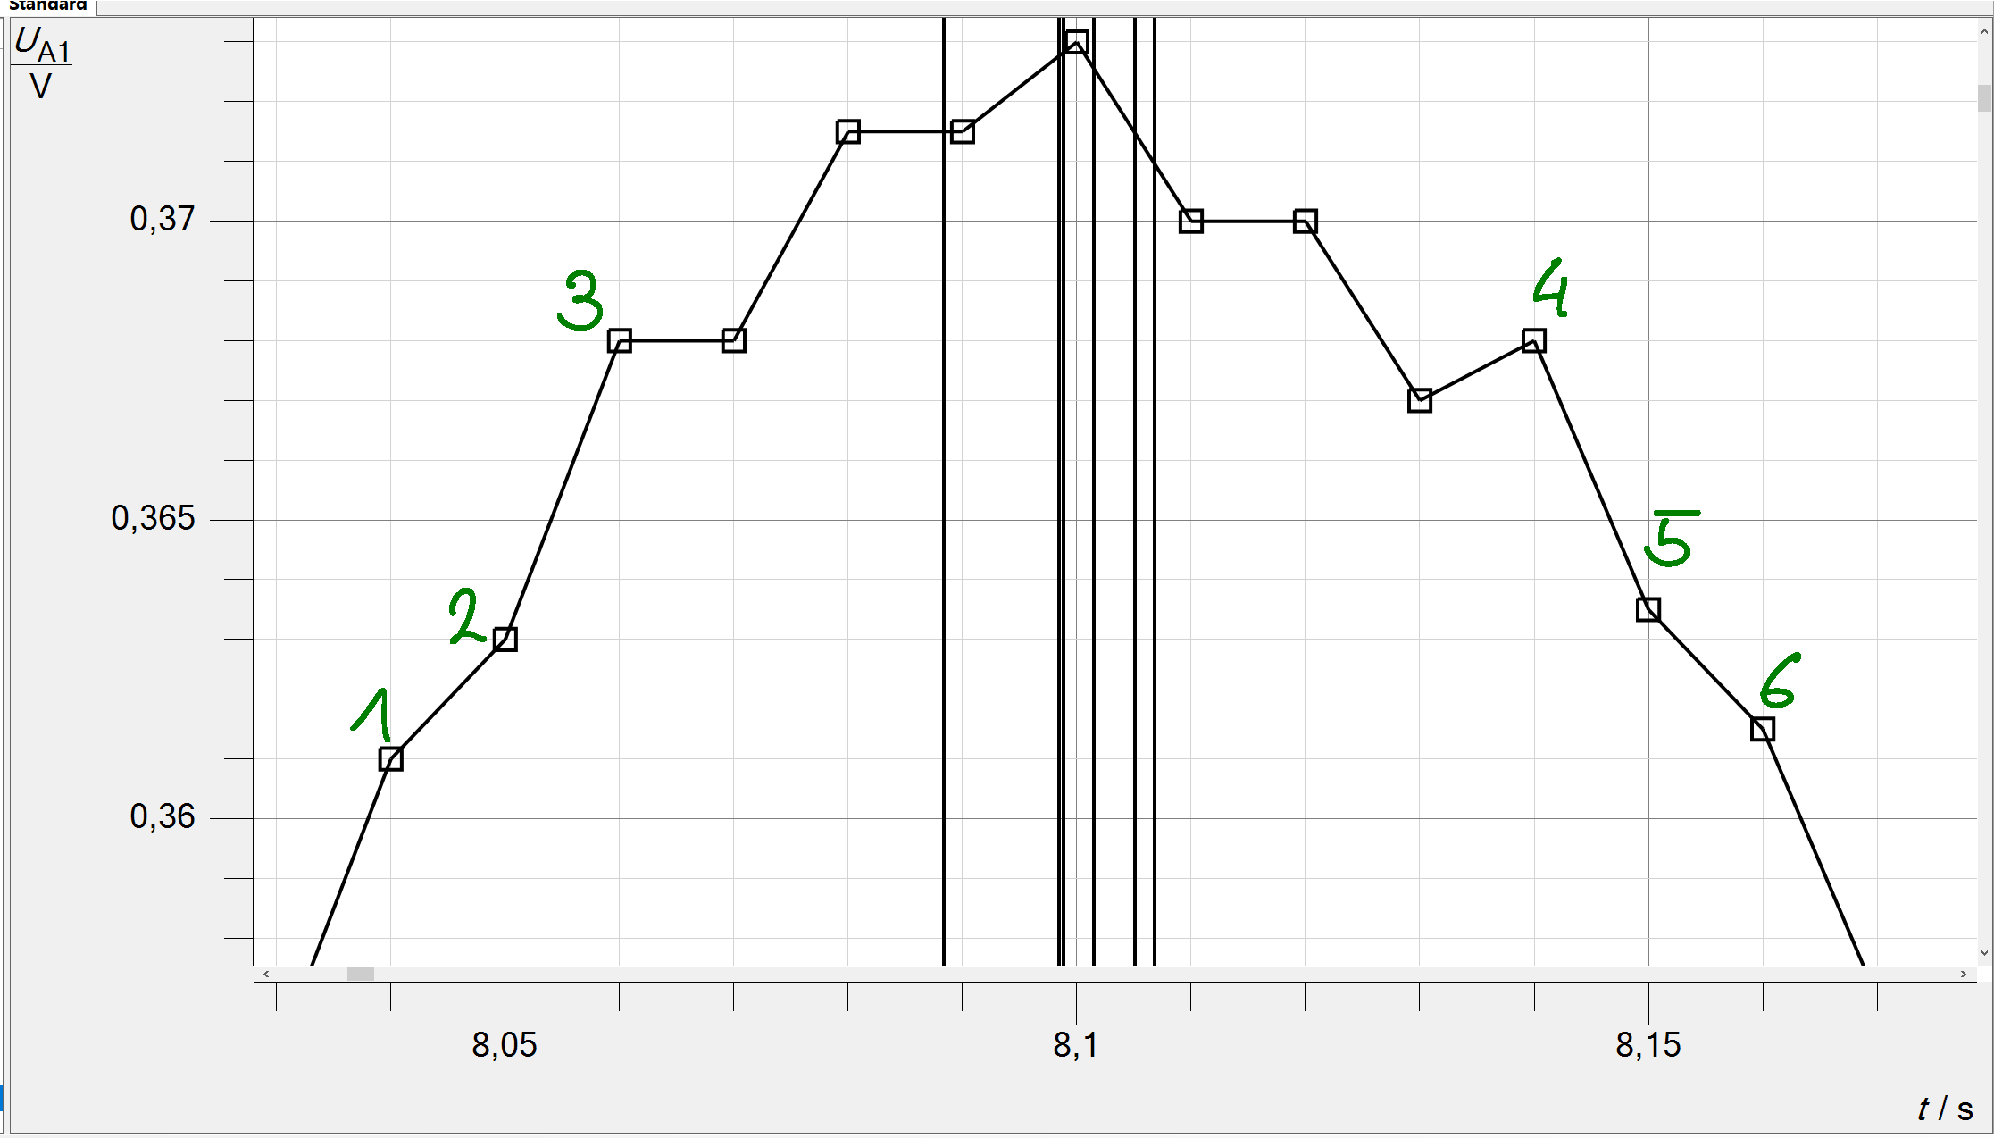
\includegraphics[width=0.8\textwidth]{plots/unsicherheit-bestimmen-stange1-punkte.pdf}
    \caption{Peakfinder Variation der Grenzen bei Messung Stange 1}     
\end{figure}
Zuerst haben wir als Grenzen 3-4, 2-5 und 1-6 genommen, da diese Punkte immer in etwa auf der gleichen Höhe lagen.
Da wir beim Auswerten aber nicht immer Punkte auf der gleichen Höhe nehmen konnten, haben wir auch noch leicht verschobene Grenzen gewählt.
Dies war auch nötig, damit in der anschließenden Fehlerbestimmung für die Streuung ein Realistischer Wert herauskommt.
Darum haben wir noch die Kombinationen 1-5, 5-3 und 2-6 genommen.
Anschließend haben wir den Mittelwert gebildet.
Dieses ist Sinnvoll, da alle Peaks gleichwarscheinlich sind, entsprechend können wir sie alle gleich gewichten.
Anschließend haben wir eine konservative Fehlerabschätzung gemacht, indem wir die Differenz zu dem Wert genommen haben, welcher am stärksten vom Mittelwert abweicht.
Diese Differenz haben wir dann als Fehler angenommen.
Dabei haben wir diesen Fehler auf die Zeit für alle bestimmten Peaks von der Messung angenommen.
Dies ist eine valide Annahme, da wir bei allen Peaks die gleiche Auflösung in der Zeit und der Spannung haben, und auch alle Peaks mit der gleichen Methode abgelesen haben.
Auch die Einflussfaktoren auf das Pendel, wärend der Versuchszeit (Dämpfung Erschütterungen etc.) waren nicht so groß, dass sie einen Einfluss auf den Fehler haben werden.

\begin{figure}[H]
    \centering
    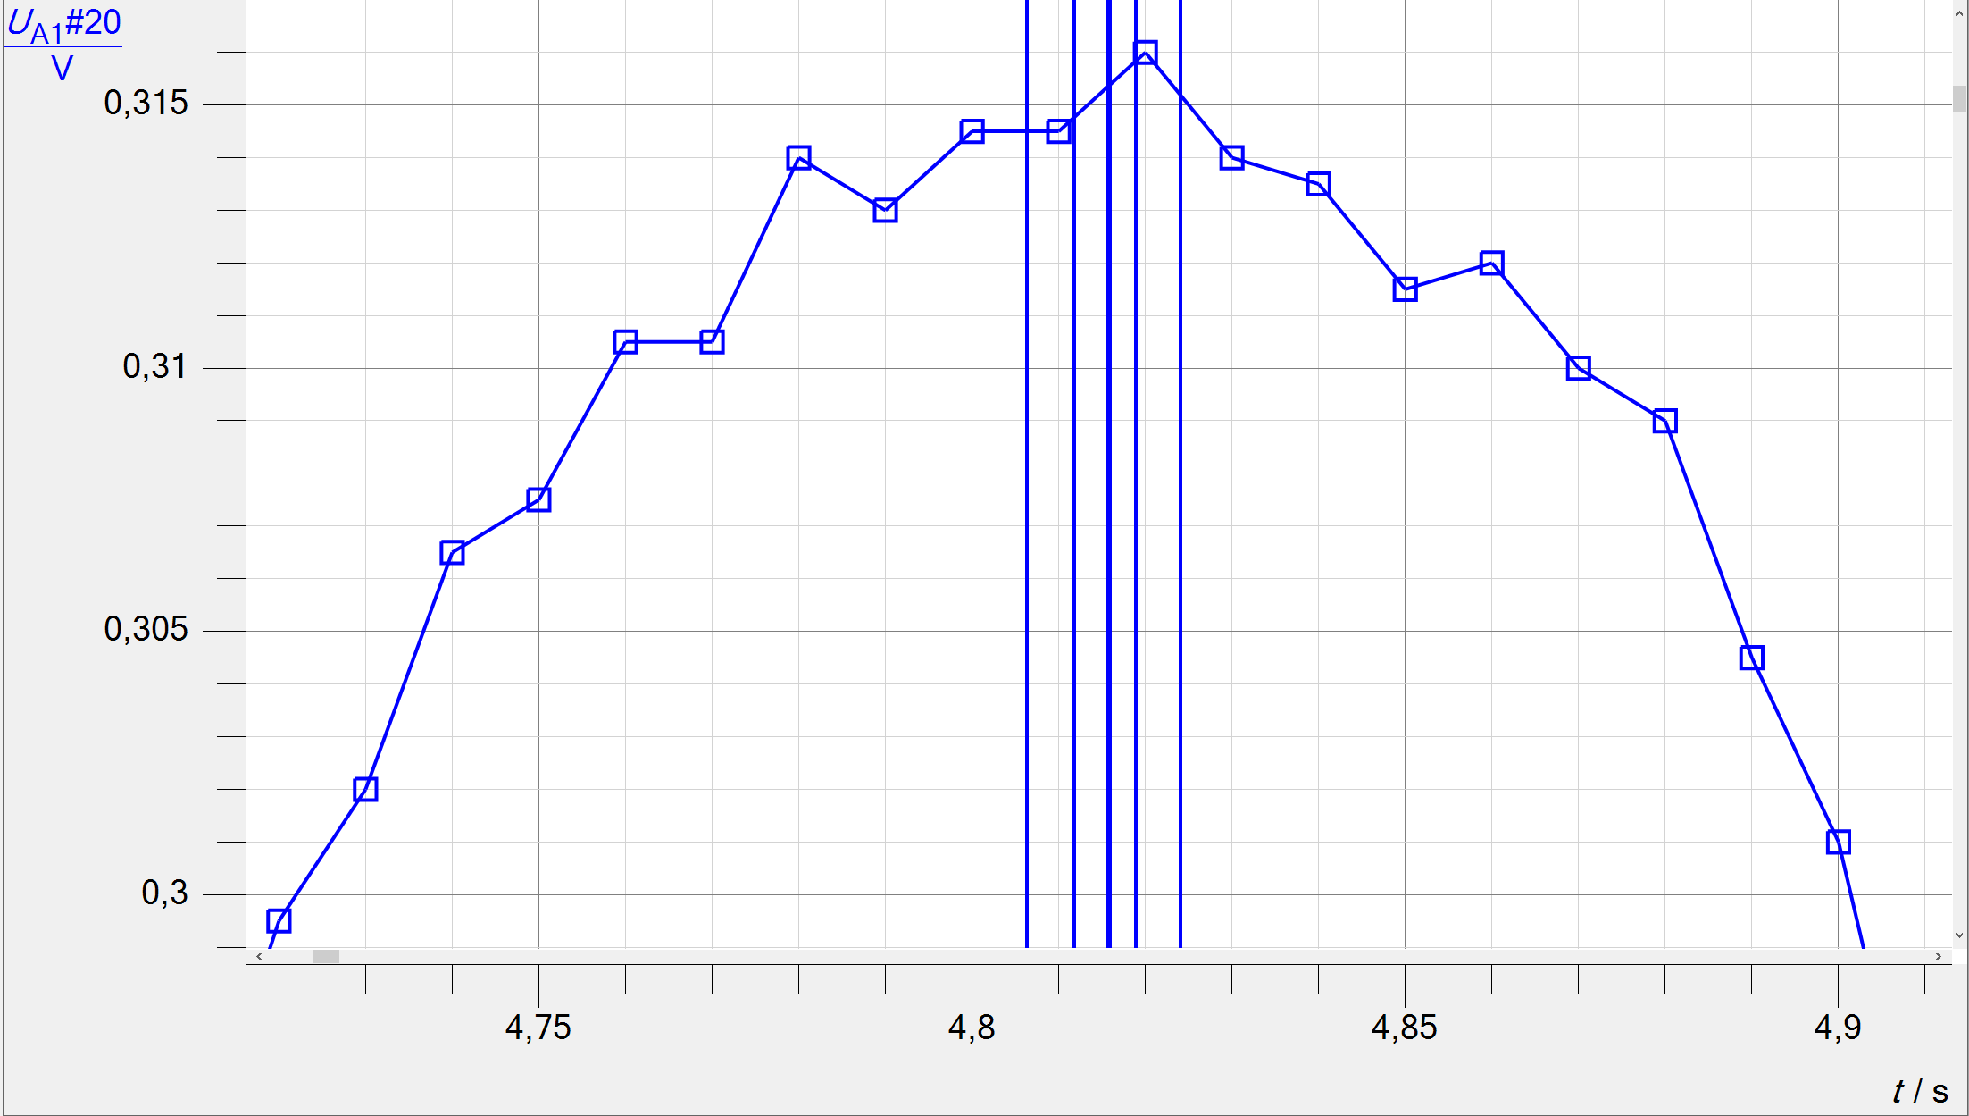
\includegraphics[width=0.8\textwidth]{plots/unsicherheit-bestimmen-gewicht-1.pdf}
    \caption{Peaks bei Messung Pendel mit Gewicht 1}
\end{figure}

Hier noch eine Grafik wo wir den Fehler auf die Zeit der ersten Messung mit Pendelkörper bestimmt haben. 
Hier sind wir gleich vorgegangen wie oben erklärt. 

\subsection{Bestimmung der Periodendauer}
Wir haben jede Messung (3x ohne Gewicht und 3x mit) einzeln ausgewertet um die Periodendauer zu bestimmen.
Für jede Messung haben wir über 110 Perioden aufgezeichnet und diese auch ausgewertet. 
Zur Auswertung haben wir immer in etwa jeden 10. Peak den Zeitpunkt bestimmt, sodass wir insgesamt 12 Peaks für jede Messung haben.
Dies sind somit schon genug Messungen um anschließend Sinnvoll eine Lineare Regression durchzuführen.
Dabei haben wir aber nicht immer strikt jeden 10 Peak genommen, dabei manchen Peaks kein klares Maximum zu erkennen war.
Wenn dies der Fall war, haben wir den Peak davor oder dahinter genommen.
In der Folgenden Tabelle sind die Ergebnise von allen Messungen dargestellt.
Da wir die Auswertung mit CASSY gemacht haben, haben wir eine Messung bei welcher wir alle benötigten Maxima bestimmt haben, gesondert abgespeichert mit dem Suffix "mit-maxima".
Dort lassen sich alle bestimmten Peaks (auch die für die Fehlerbestimmung) nachschauen.

In der Tabelle ist N der Index des Maximums, also das wievielte Maximum vorliegt , in der Spalte rechts daneben ist der Zeitpunkt dieses Maxima eingetragen.

\begin{table}[H]
    \centering
    \begin{tabularx}{1.0\textwidth}{X X X X X X}
       \textbf{N}  & \textbf{Stange 1} & \textbf{N} & \textbf{Stange 2} & \textbf{N} & \textbf{Stange 3} \\
       \toprule
       2 & 3.138s &  1 & 1.455s &  1 & 1.528s \\
       11 & 18.063s &  10 & 16.382s &  11 & 18.088s \\
       20 & 32.935s &  20 & 32.944s &  20 & 33.022s \\
       30 & 49.473s &  29 & 47.857s &  29 & 47.909s \\
       40 & 66.058s &  39 & 64.411s &  39 & 64.471s \\
       50 & 82.598s &  50 & 82.628s &  51 & 84.347s \\
       60 & 99.19s &  60 & 99.192s &  60 & 99.269s \\
       70 & 115.729s &  69 & 114.075s &  69 & 114.162s \\
       79 & 130.651s &  80 & 132.288s &  79 & 130.7s \\
       90 & 148.843s &  90 & 148.857s &  90 & 148.936s \\
       101 & 167.079s &  100 & 165.417s &  101 & 167.164s \\
       112 & 185.279s &  111 & 183.626s &  111 & 183.715s \\
       \midrule
        & \textbf{$\sigma_{Stange-1-stat}$} & & \textbf{$\sigma_{Stange-2-stat}$} & & \textbf{$\sigma_{Stange-3-stat}$} \\
       \midrule
        & 0.0115s & & 0.0072s & & 0.0110s \\
       \toprule
    \end{tabularx}
    \caption{Maxima \& stat Fehler bei Messung des Pendels ohne Pendelkörper}
\end{table}

 
 
\begin{table}[H]
    \centering
    \begin{tabularx}{1.0\textwidth}{X X X X X X}
       \textbf{N}  & \textbf{Gewicht 1} & \textbf{N} & \textbf{Gewicht 2} & \textbf{N} & \textbf{Gewicht 3} \\
       \toprule
       1 & 1.508s &  1 & 1.636s &  1 & 1.59s \\
       11 & 18.062s &  11 & 18.176s &  12 & 19.772s \\
       21 & 34.581s &  21 & 34.733s &  21 & 34.653s \\
       31 & 51.141s &  31 & 51.253s &  30 & 49.539s \\
       41 & 67.679s &  39 & 64.501s &  39 & 64.445s \\
       50 & 82.562s &  50 & 82.71s &  50 & 82.636s \\
       60 & 99.13s &  60 & 99.246s &  59 & 97.518s \\
       70 & 115.653s &  69 & 114.136s &  69 & 114.06s \\
       79 & 130.521s &  82 & 135.616s &  80 & 132.239s \\
       91 & 150.368s &  91 & 150.532s &  90 & 148.788s \\
       99 & 163.627s &  100 & 165.394s &  101 & 166.969s \\
       108 & 178.526s &  111 & 183.606s &  110 & 181.893s \\
       \midrule
        & \textbf{$\sigma_{Gewicht-1-stat}$} & & \textbf{$\sigma_{Gewicht-2-stat}$} & & \textbf{$\sigma_{Gewicht-3-stat}$} \\
       \midrule
        & 0.0095s & & 0.0096s & & 0.0084s \\
       \toprule
    \end{tabularx}
    \caption{Maxima \& stat Fehler bei der Messung des Pendels mit Pendelkörper}
\end{table}

Wie zu sehen ist, hat sich das bestimmen der verschiedenen Statistischen Fehler gelohnt, da diese zum teil sehr unterschiedlich sind.
Das sie so unterschiedlich sind, kann aber auch zufall sein, da wir immer einen zufälligne Peak untersucht haben.\\

\subsubsection{Bestimmen von T des Pendels ohne Pendelkörper}
Anschließend haben wir N (auf der x-Achse) gegen die Zeit (y-Achse) geplottet.
Dabei gibt es keinen Fehler auf N, da wir davon ausgehen das wir uns nicht verzählt haben.
Der Fehler auf die Zeit ist dabei der statistische Fehler vom ablesen.

Anschließend haben wir eine lineare Regression gemacht.
Dabei ist die Steigung der Geraden die Periodendauer.
Der Fehler auf die Periodendauer ist dann der Fehler auf die Steigung welchen wir aus der linearen Regression erhalten.
Im folgenden werden Sämtliche lineare Regressionen dargestellt.
Im obere Graph ist immer die Anzahl gegen die Zeit aufgetragen. 
Der untere Graph stellt die Abweichung unserer Werte von der linearen Regression dar. 
\begin{figure}[H]
    \centering
    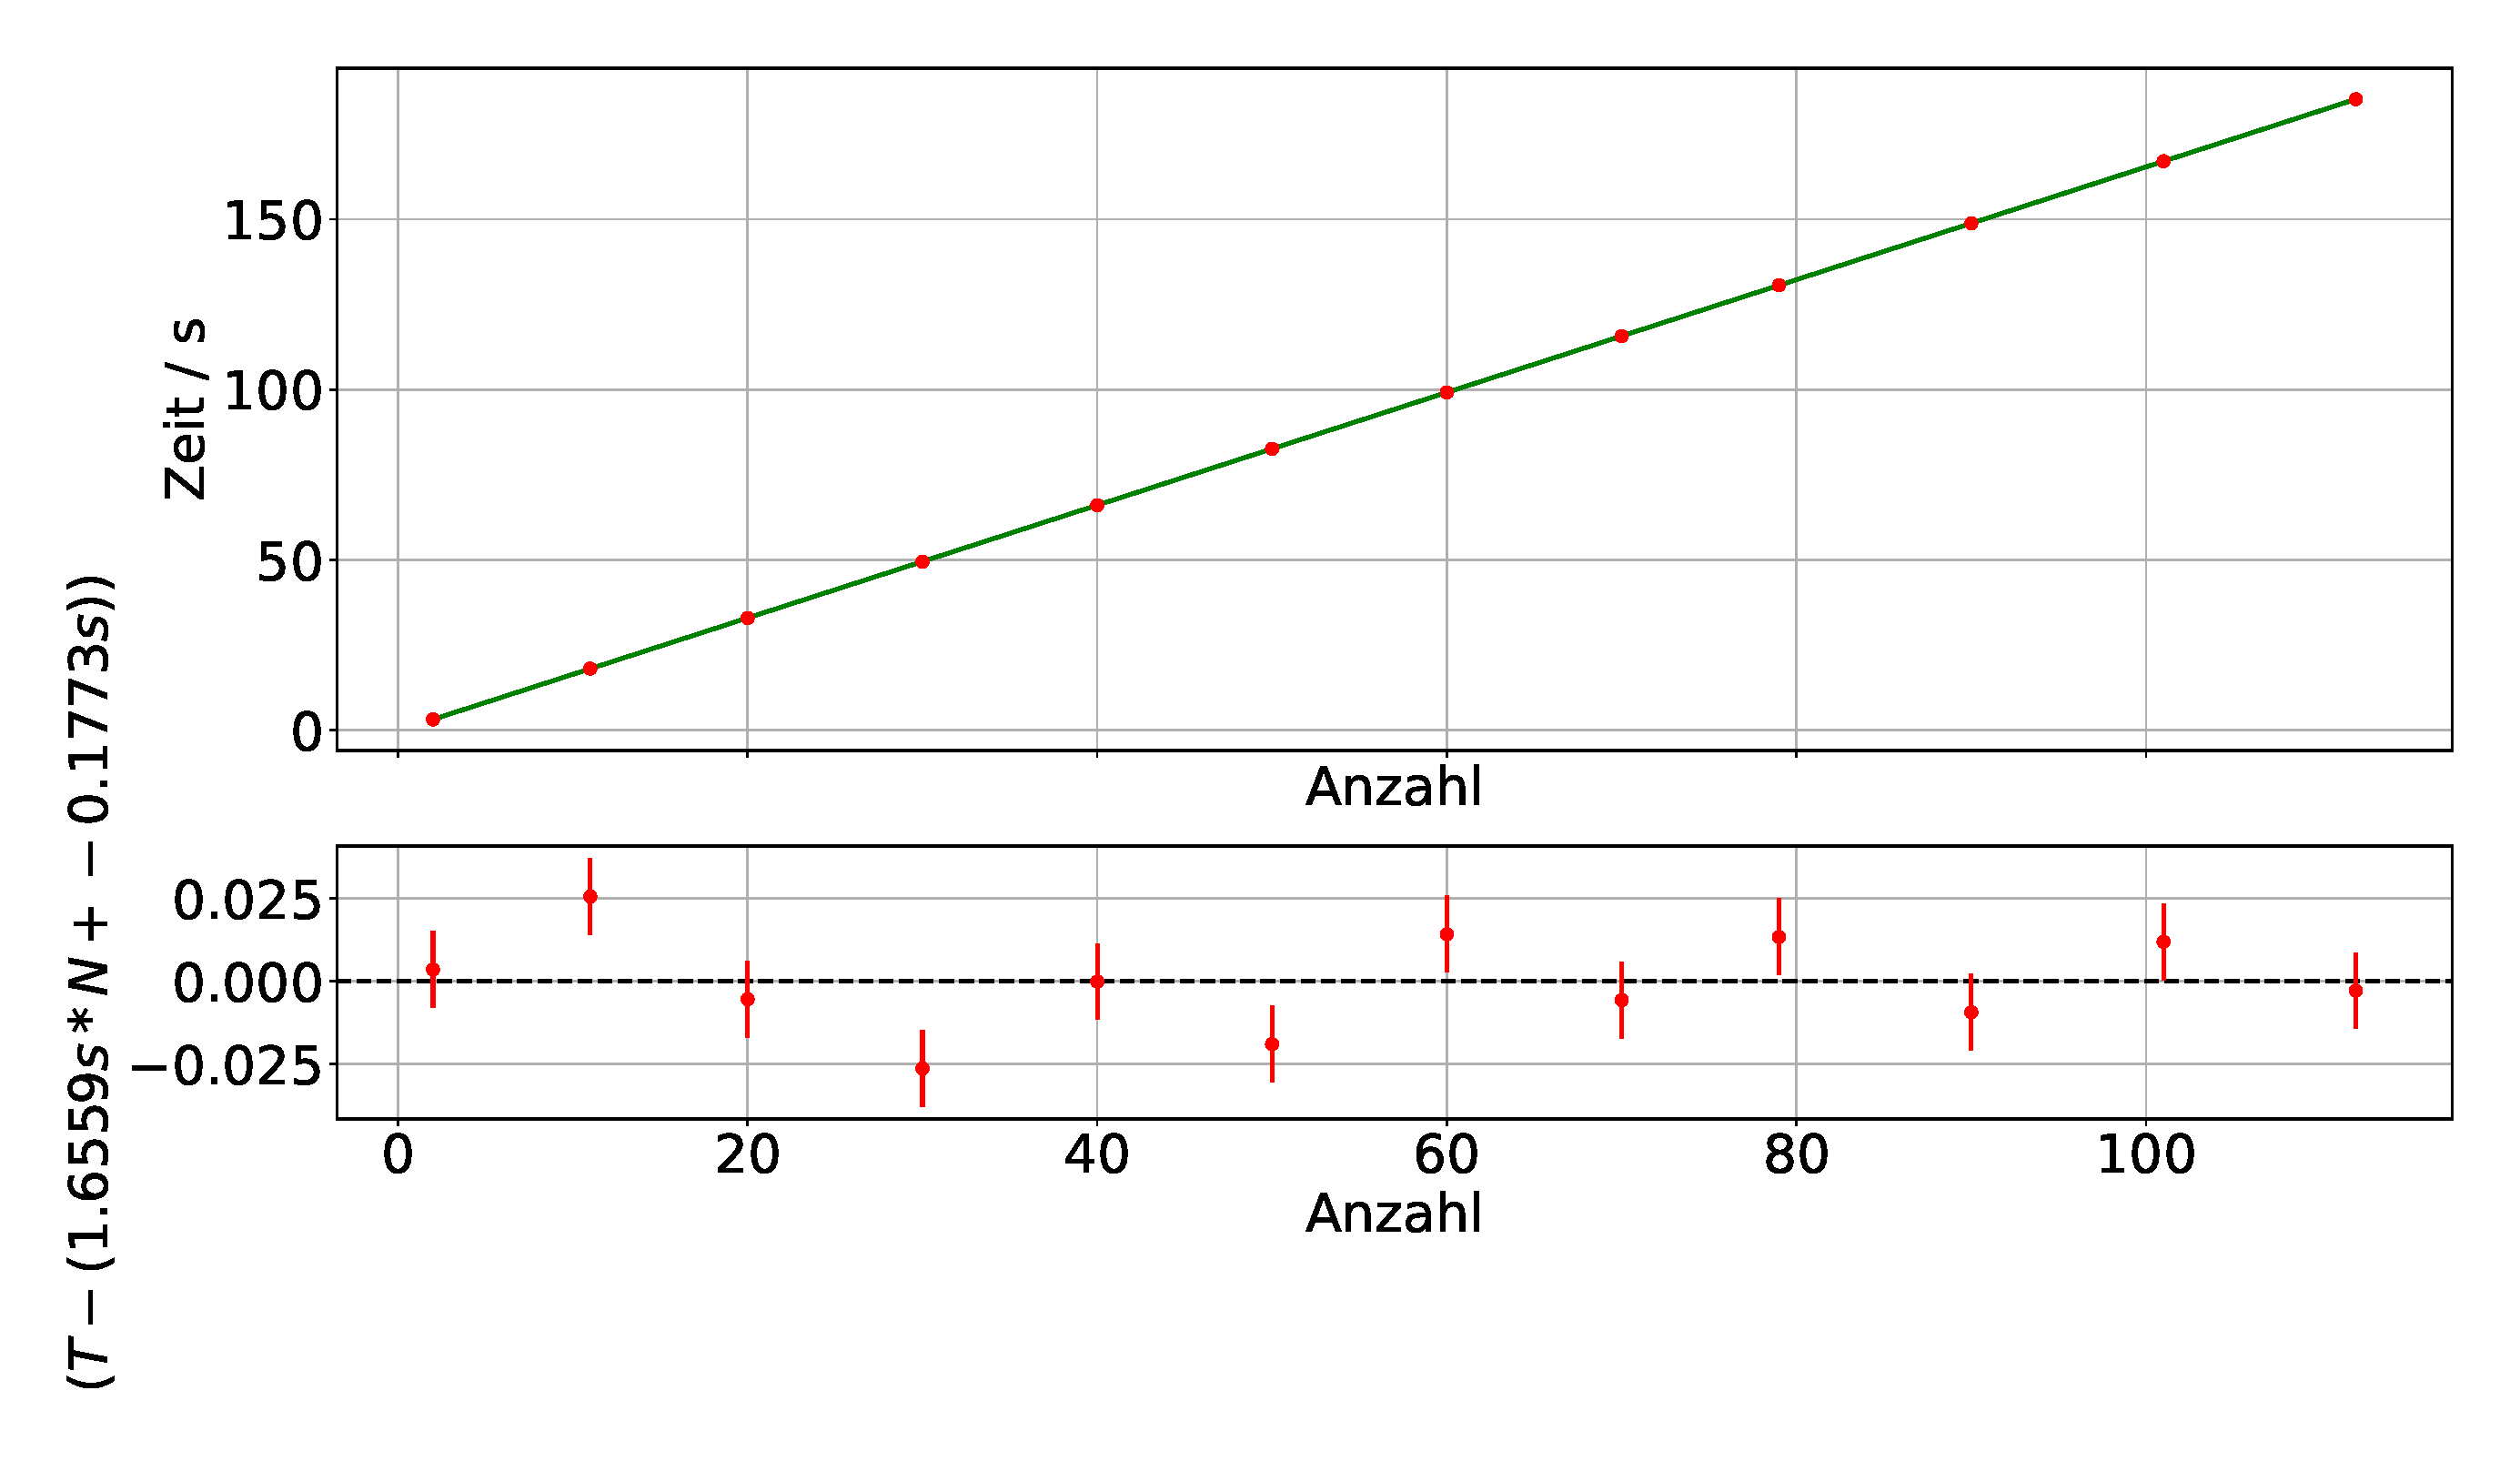
\includegraphics[width=1.0\textwidth]{plots/lineare_regression_stange_1.pdf}
    \caption{1. Messung ohne Pendelkörper mit Lineare Regression und Residuen Plot}
\end{figure}
\begin{center}
    $ \frac{\chi^2}{ndof}  =  1.8$
\end{center}

Im obigen Graphen der 1. Messung ohne Pendelkörper sieht man, wie die gemessene Zeit für N Perioden linear ansteigt.
Daran kann man erkennen, dass das anpassen einer linearen Funktion an die Messpunkte eine sinnvolle Herangehensweise ist.
Im unteren Graphen ist der Residuen Plot zu sehen. Hier haben wir auf der y-Achse die Differenz von gemessener Zeit und der mit der Linaren Regression errechnete Zeit aufgetragen. 
Auf der x-Achse ist ebenfalls N aufgetragen.
Im Residuen Plot liegt keine Systematik vor, was für eine gute Anpassung spricht.
Zudem gibt es keine Ausreißer, da kein Messwert weiter als $3\sigma$ von der Anpassung entfernt ist.
Nach Augenmaß liegen 6 Messwerte weniger als $1\sigma$ von der Anpassung entfernt. Dies ist etwas weniger als man bei einer Normalverteilung erwarten würde hier sollten 68\% innerhalb einer Standardabweichung liegen. Es liegen jedoch 95\% innerhalb von zwei Standardabweichungen sodass wir schließen können, dass die Messwerte normalverteilt um die Linare Regression streuen.
Das $\chi^2$ ist zwar größer als 1, was bedeutet das wir unsere Messfehler etwas unterschätzt haben, aber immer noch gut das es kleiner als 3 ist.
Der y-Achsenabschnitt ist $ (-0.1773 \pm 0.0063)s$, was gegenüber der Messdauer von über 180s und einer Periodendauer von ca 1.65s  klein ist.
Aus der Steigung ergibt sich $T = (1.6559 \pm 0.0001)s$, was mit unseren überschlagenen Werten von 1.65s übereinstimmt.
Damit handelt es sich um eine gute Anpassung.
 
\begin{figure}[H]
    \centering
    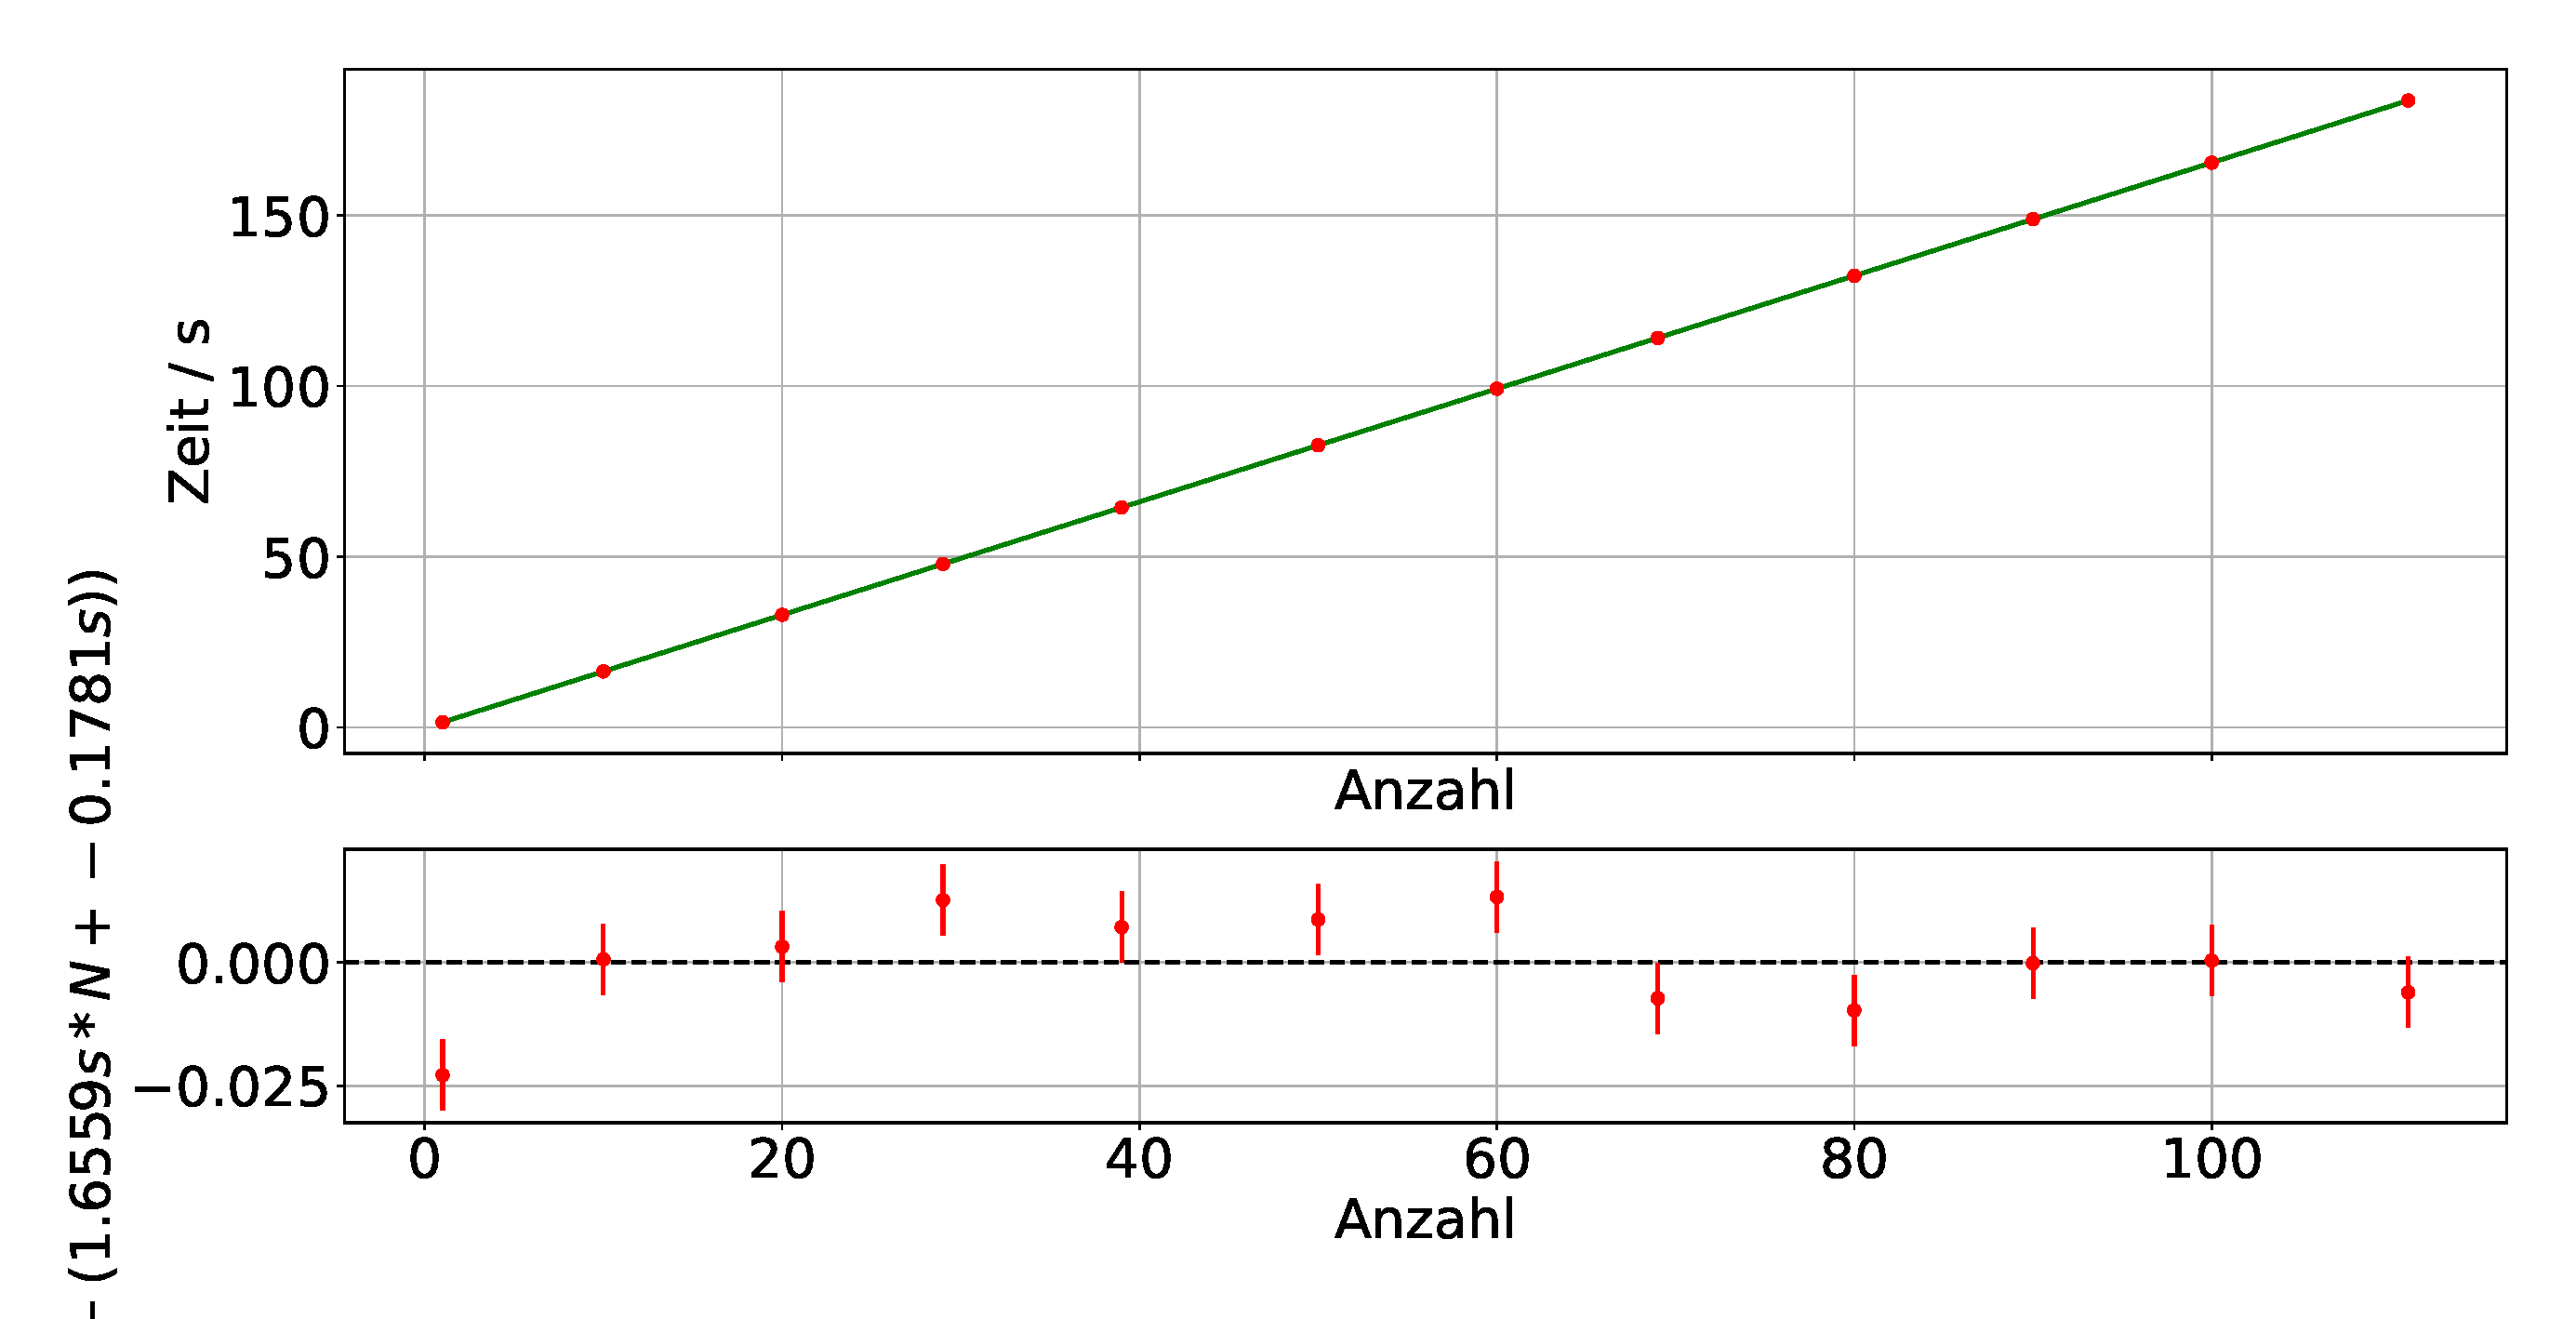
\includegraphics[width=1.0\textwidth]{plots/lineare_regression_stange_2.pdf}
    \caption{2. Messung ohne Pendelkörper mit Lineare Regression und Residuen Plot}
\end{figure}
\begin{center}
    $ \frac{\chi^2}{ndof}  =  2.3$
\end{center}
Im oberen Graphen der 2. Messung von der Stange sieht man, wie die gemessene Zeit für N Perioden linear ansteigt.
Im Residuen Plot könnte der 1. Wert ein Ausreißer sein, er liegt aber knapp weniger als $3\sigma$ von der Anpassung entfernt.
Die anderen Werte streuen statistisch um die Anpassung und es liegt keine systematische Abweichung vor.
Dem $\chi^2$ zufolge haben wir die Messfehler leicht unterschätzt, aber immer noch gut das es kleiner als 3 ist.
Folglich ist es eine gute Anpassung und die Wahl der Linaren Regression war richtig.
Mit $b = (-0.1781 \pm 0.0039)s$ ist dieses so wie oben Argumentiert vernachlässigbar nahe an 0.
Durch die Regression konnte die Periodendauer zu $T = (1.6559 \pm 0.0001)s$ bestimmt werden.


 
\begin{figure}[H]
    \centering
    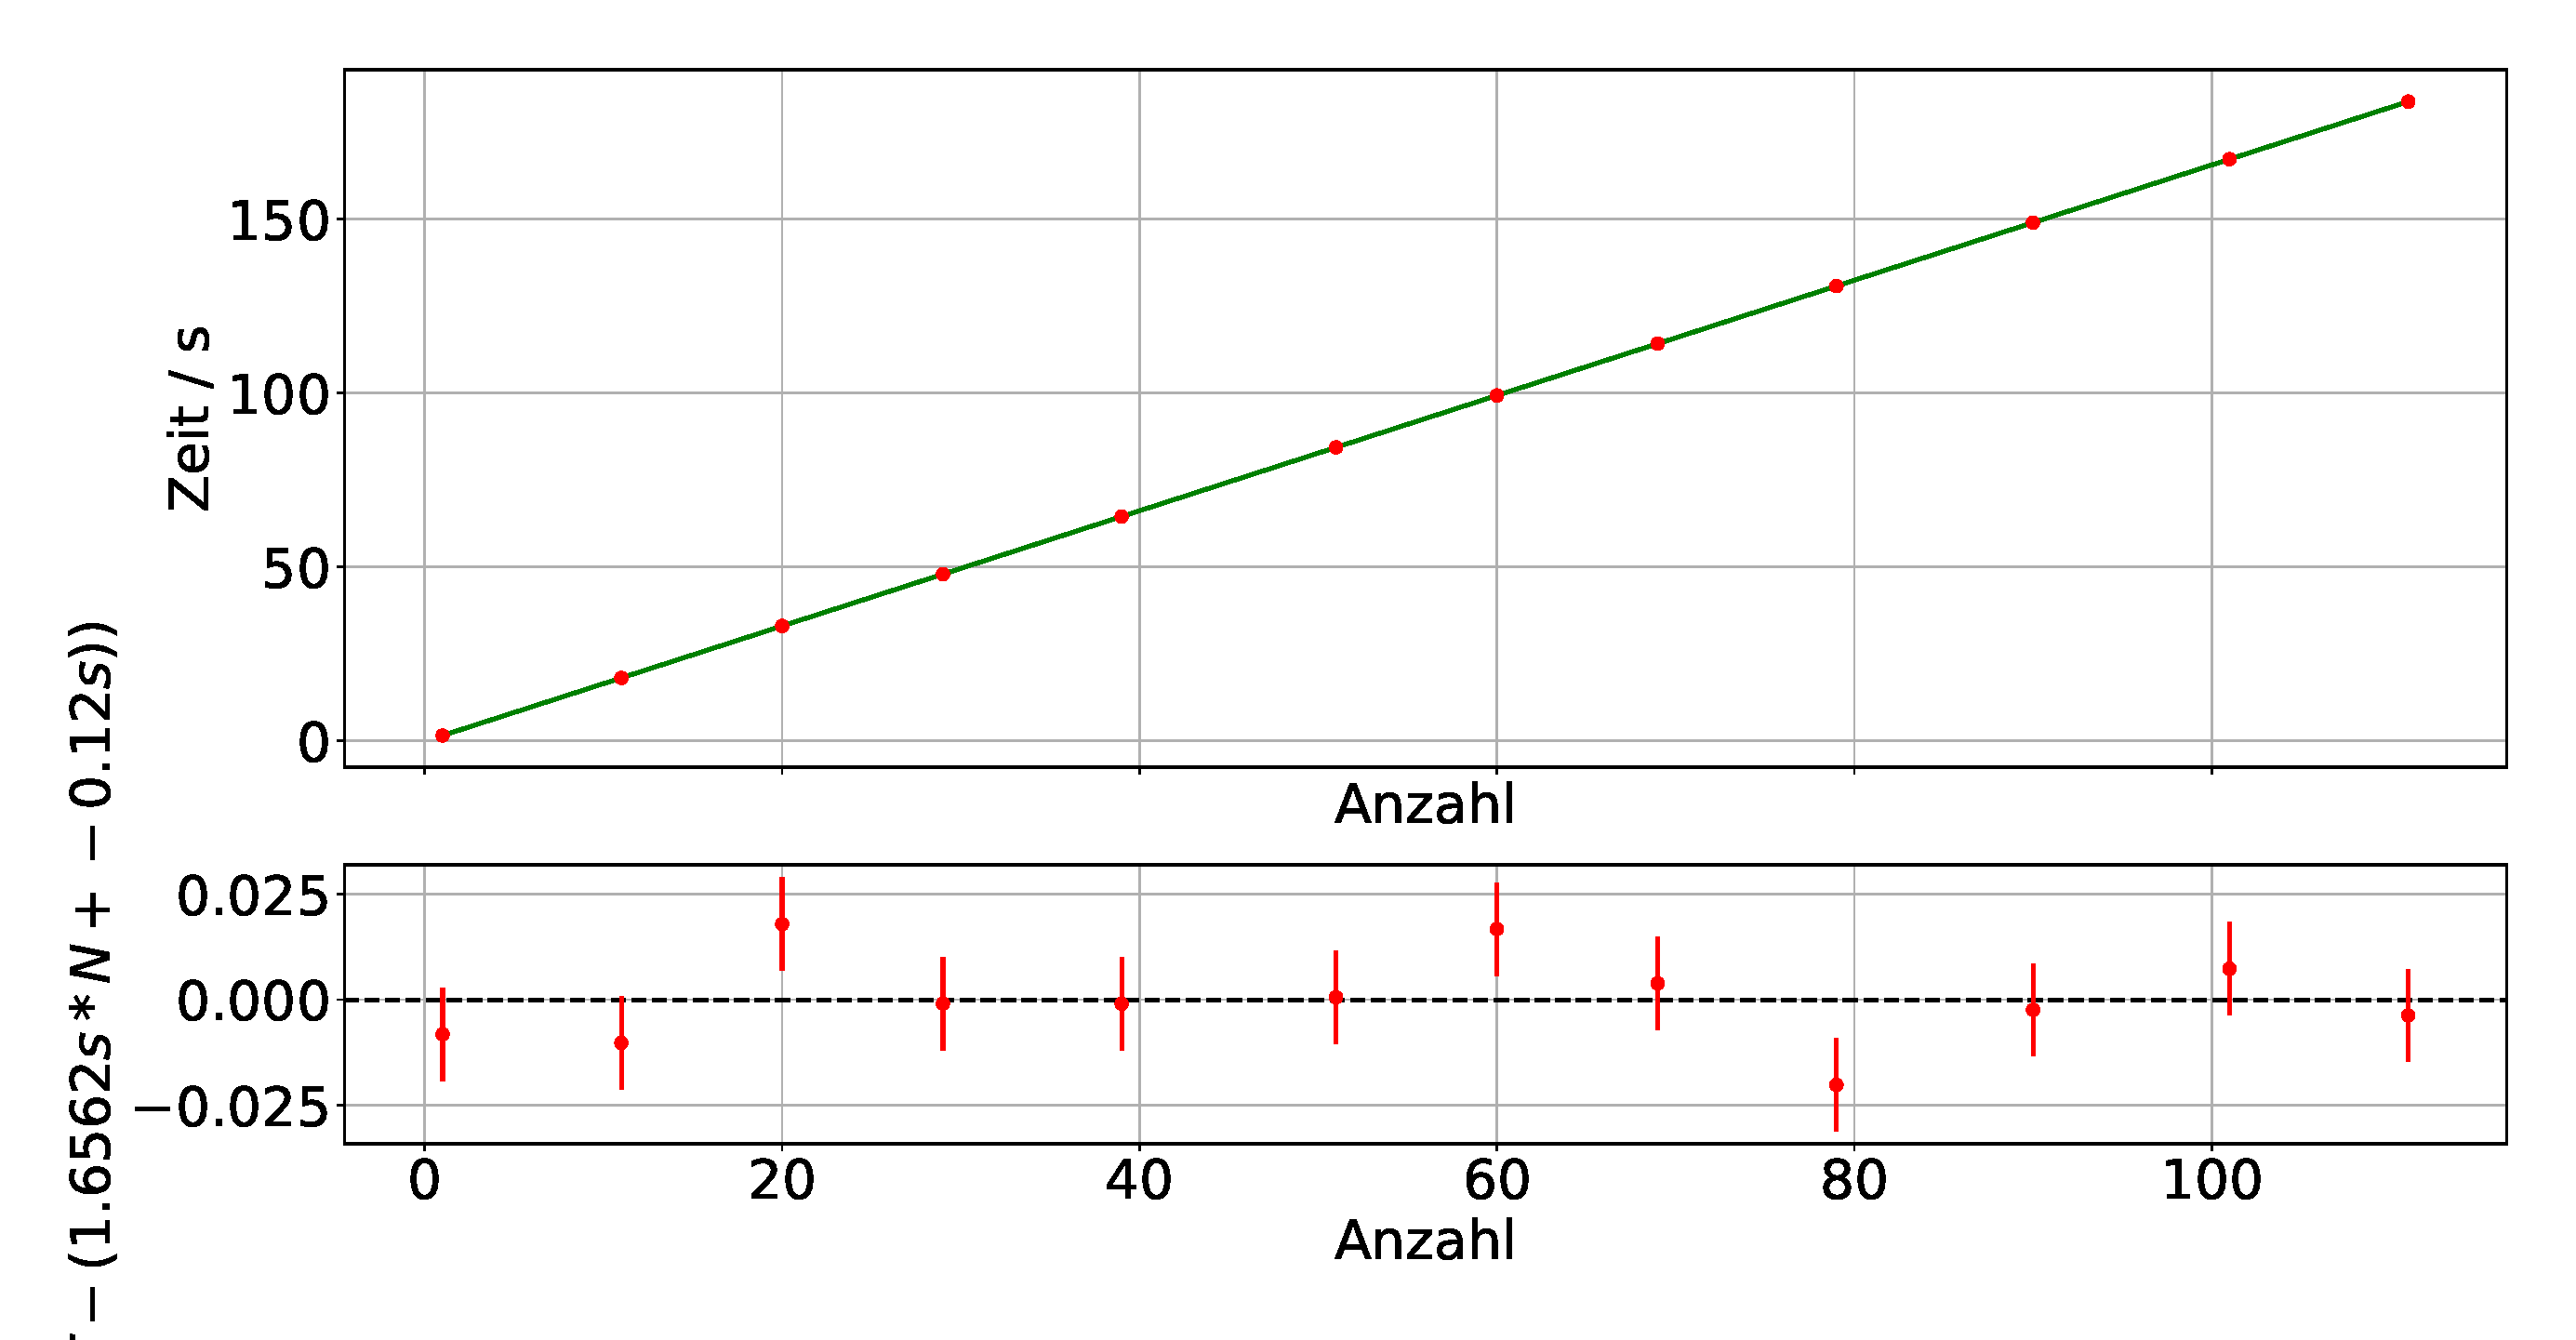
\includegraphics[width=1.0\textwidth]{plots/lineare_regression_stange_3.pdf}
    \caption{3. Messung ohne Pendelkörper mit Lineare Regression und Residuen Plot}
\end{figure}
\begin{center}
    $ \frac{\chi^2}{ndof}  =  1.0$
\end{center}
Auch hier kann man im oberen Graphen klar sehen, das die Gesamte Zeit für N Perioden linear ansteigt.
Im Residuen Plot gibt es keine Ausreißer und 3 Messwerte, welche nicht innerhalb von einer Standartabweichung von der Anpassung liegen.
Dies spiegelt sich im $\chi^2$ wieder, welches genau 1 ist und somit sehr gut.
Dabei ist der y-Achsenabschnitt $b =(-0.1200 \pm 0.0060)s$ und die Steigung $T = (1.6562 \pm 0.0001)s$.
$b$ ist dabei gegenüber der deutlich größeren Periodendauer vernachlässigbar klein.
Dies würde man auch erwarten, wenn keine Systematik vorliegt.

Zusammenfassen kann festgehalten werden, das alle Messungen vom Pendel ohne Pendelkörper gut mit einer Linearen Regression als Anpassung ausgewertet werden können, und somit über die Steigung die Periodendauer bestimmt werden kann.

Das gleiche Vorgehen wählen wir auch zur Bestimmung der Periodendauer des Pendels mit Pendelkörper.

\subsubsection{Bestimmung von T des Pendels mit Pendelkörper}

\begin{figure}[H]
    \centering
    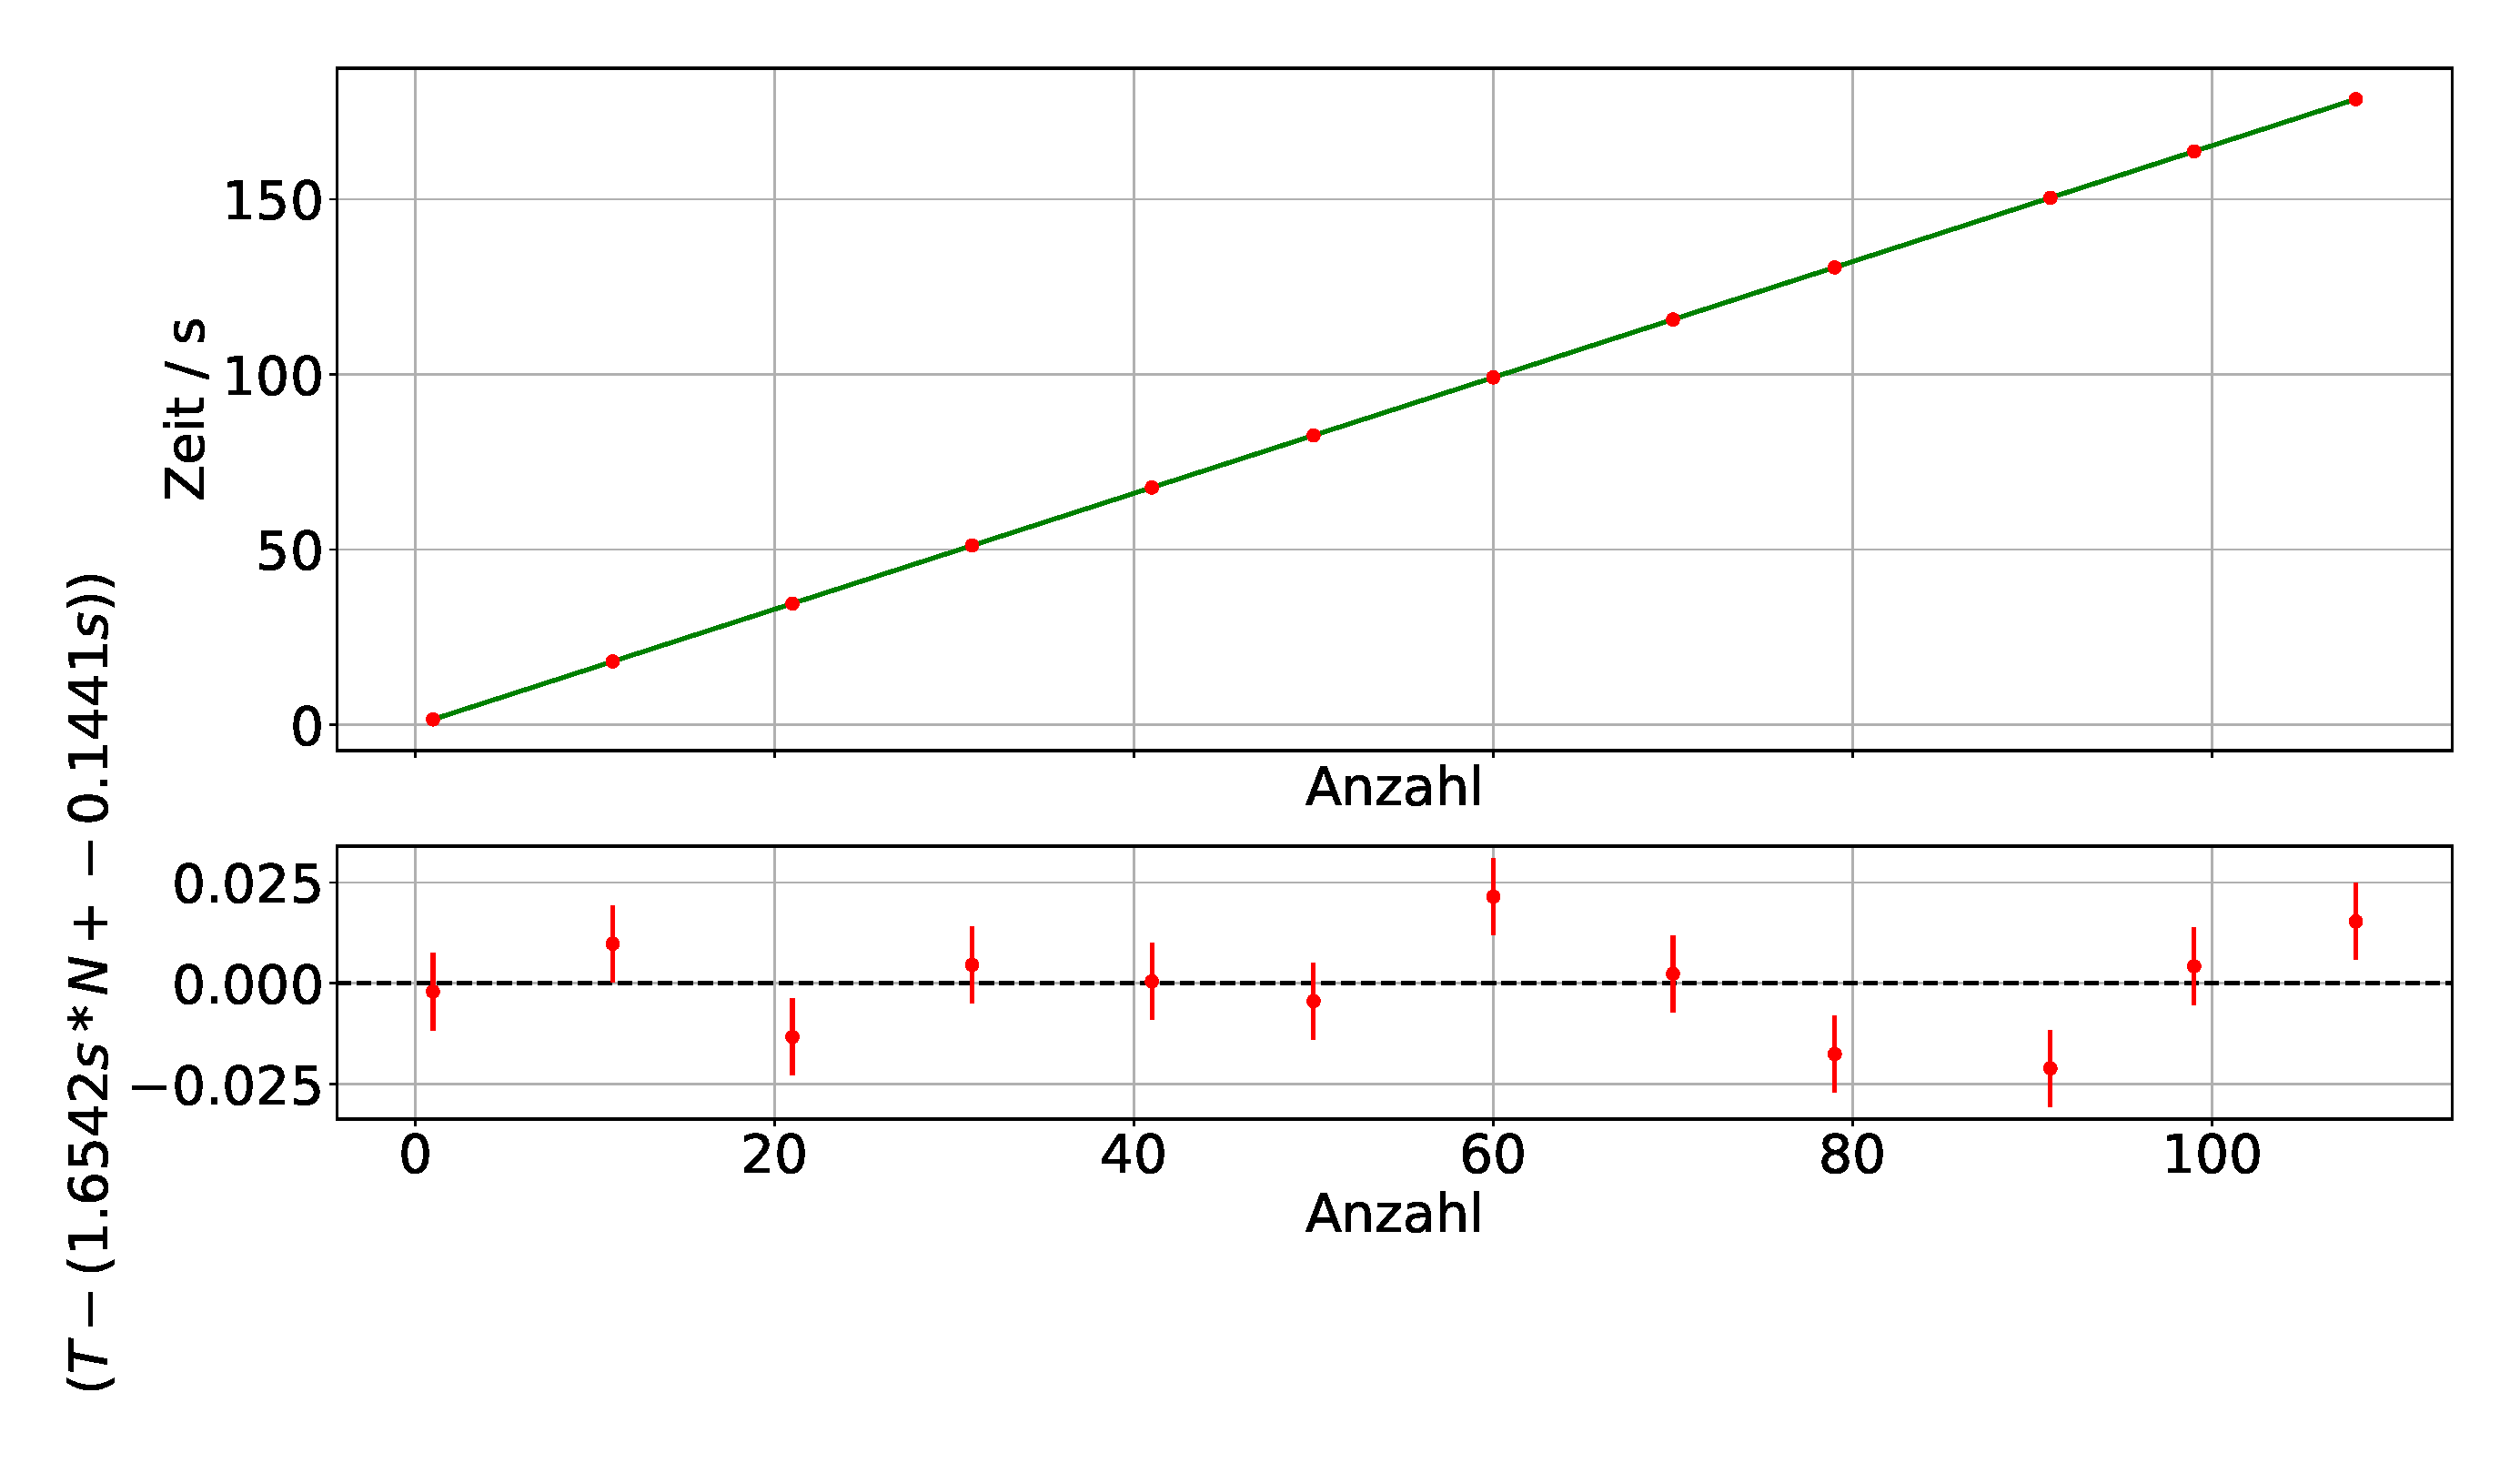
\includegraphics[width=1.0\textwidth]{plots/lineare_regression_gewicht_1.pdf}
    \caption{1. Messung mit Pendelkörper: Lineare Regression und Residuen Plot}
\end{figure}
\begin{center}
    $ \frac{\chi^2}{ndof}  =  2.0$
\end{center}
Oben sind die Messwerte für unsere erste Messung von der Stange mit Gewicht zu sehen.
Auch diese folgen einem linearen Zusammenhang.
Wie im Residuen Plot zu sehen ist, liegt keine Systematik vor.
Es ist kein Ausreißer dabei, wobei 5 Werte mehr als $1\sigma$ von der Anpassung entfernt liegen.
Dies ist aber noch akzeptabel, und da das $\chi^2$ kleiner als 3 ist, haben wir den Messfehler auch nicht unterschätzt.
$b = (-0.1441 \pm 0.0053)s$ ist gegenüber der Periodendauer von ca 1.65s und der Messdauer von 180s sehr klein.
Die Periodendauer für die erste Messung vom Pendel mit Gewicht ist $T = (1.6542 \pm 0.0001)s$.

\begin{figure}[H]
    \centering
    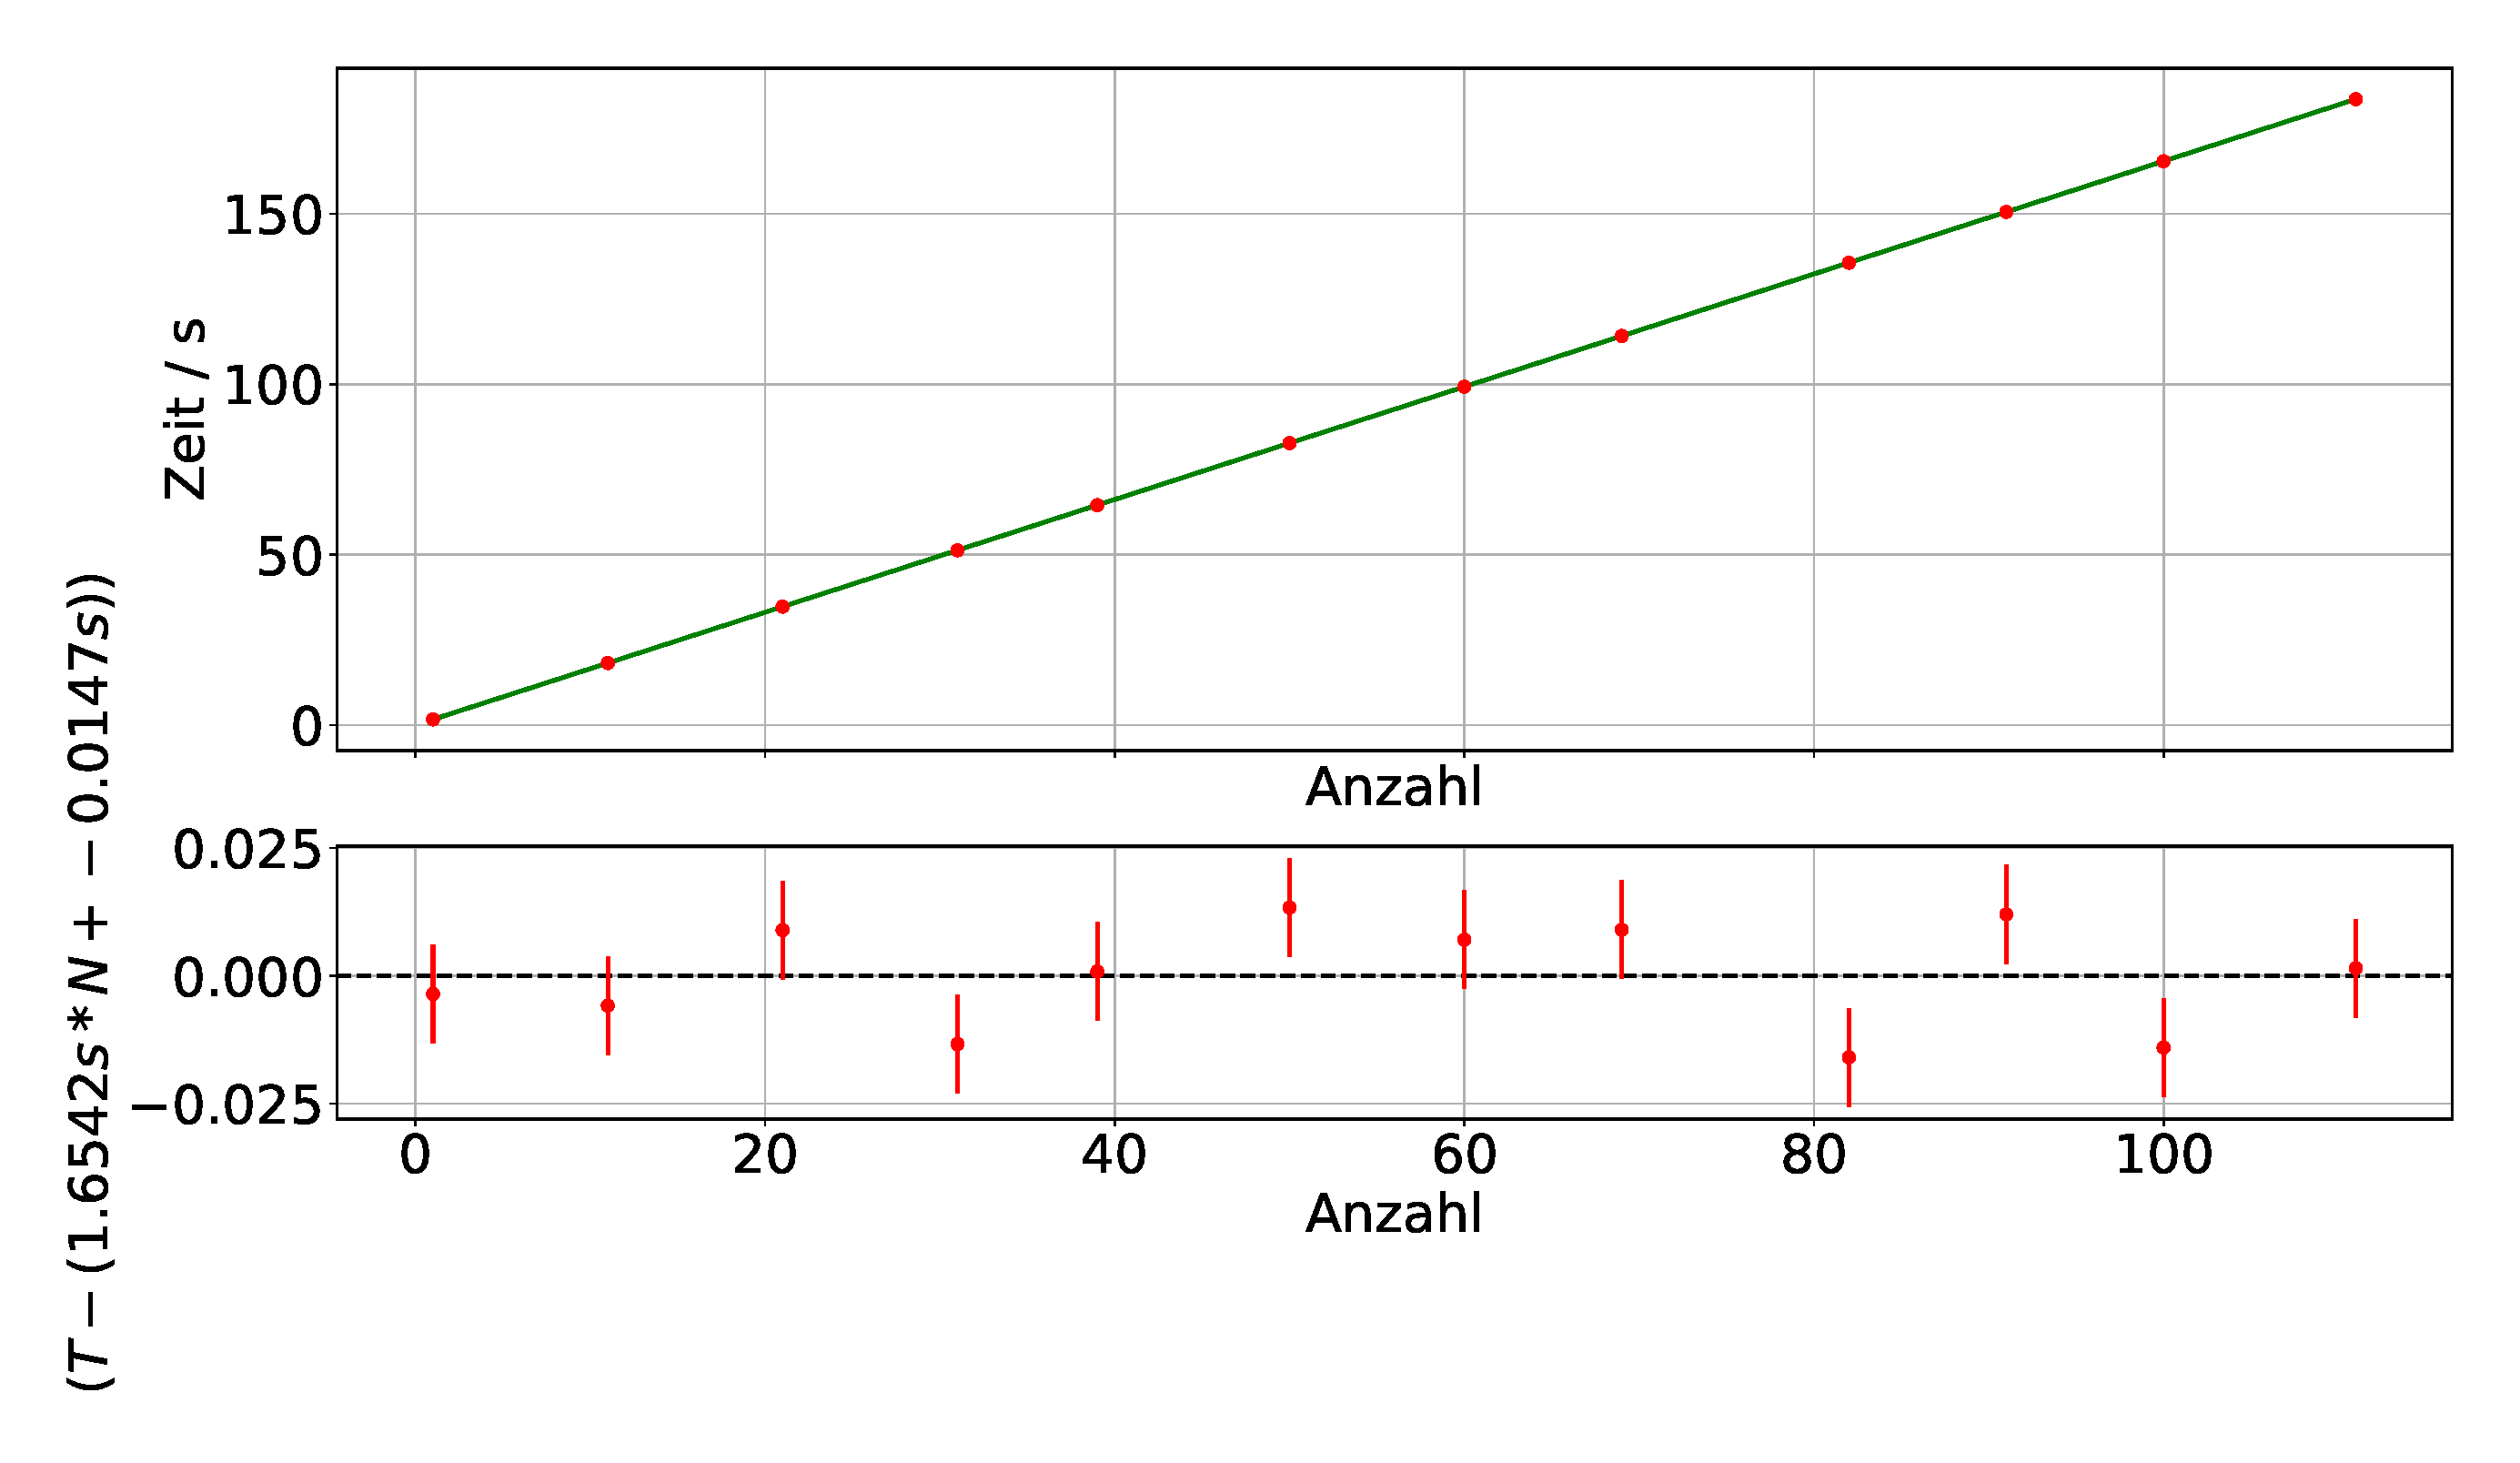
\includegraphics[width=1.0\textwidth]{plots/lineare_regression_gewicht_2.pdf}
    \caption{2. Messung mit Pendelkörper: Lineare Regression und Residuen Plot}
\end{figure}
\begin{center}
    $ \frac{\chi^2}{ndof}  =  1.3$
\end{center}
Wie im oberen Plot zu sehen ist, sind die Messpunkte linear angeordnet.
Entsprechend wurde eine Lineare Regression durchgeführt.
Wie dem Residuen Plot zu entnehmen ist, gibt es keine Systematik.
Es gibt keine Ausreißer und alle Werte streuen statistisch um die Lineare Regression.
Die Fehler haben wir leicht zu groß abgeschätzt, aber immer noch gut, da das $\chi^2$ kleiner 3 ist. Dies ist eine sehr gut Anpassung.
Aus der Linearen Regression ergibt sich $b = (-0.0147 \pm 0.0053)s$ und $T = (1.6542 \pm 0.0001)s$.
Diese Werte sprechen beide für eine sehr gute Anpassung.

\begin{figure}[H]
    \centering
    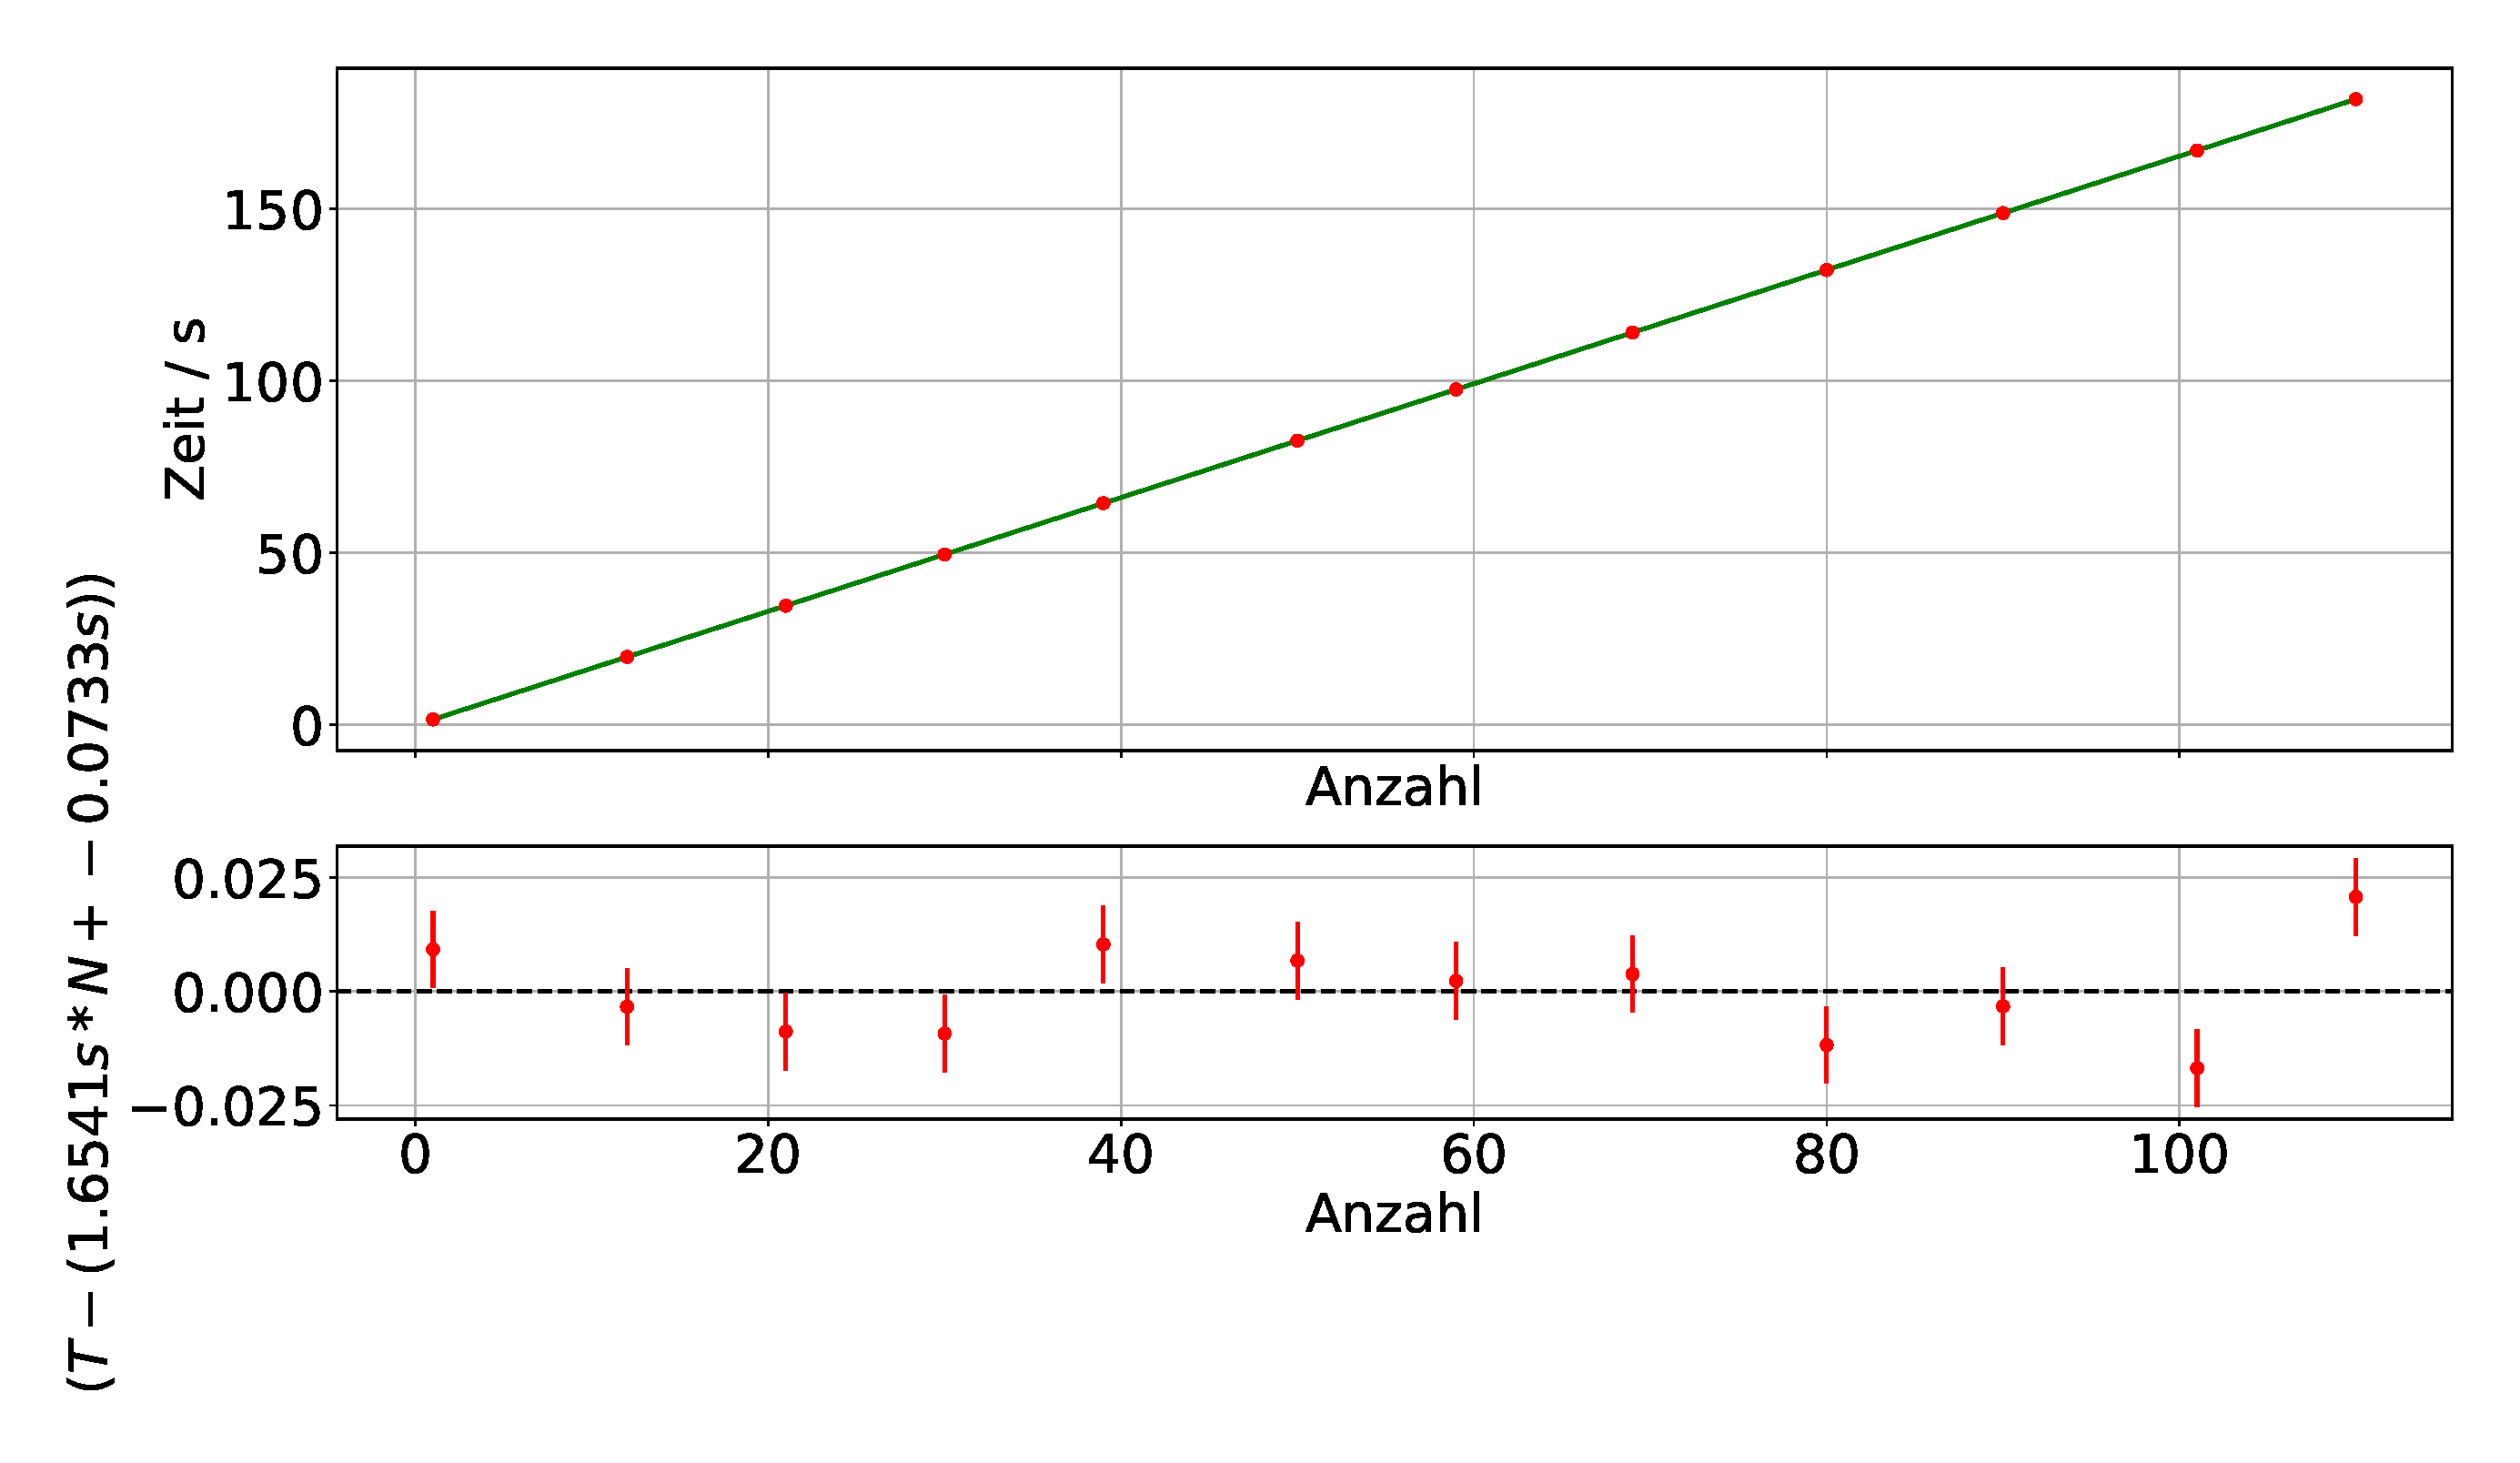
\includegraphics[width=1.0\textwidth]{plots/lineare_regression_gewicht_3.pdf}
    \caption{3. Messung von der Stange + Gewicht mit Lineare Regression und Residuen Plot}
\end{figure}
\begin{center}
    $ \frac{\chi^2}{ndof}  =  1.8$
\end{center}
Auch hier ist im oberen Plot zu sehen, wie die Messwerte einem linearen Verlauf folgen.
Im Residuen Plot ist keine Systematik zu erkennen, was bedeutet, dass unsere Anpassung zum tatsächlichen funktionalen Zusammenhang passt.
Es liegen 3 Werte nicht innerhalb von $1\sigma$, aber keiner von diesen ist ein Ausreißer. Damit sind die Messwerte wie es sein sollte normalverteilt um die Anpassung.
Das $\chi^2$ ist mit 1.8 nahe an 1 uns wir haben somit eine gute Anpassung. 
$b = ( -0.0733 \pm 0.0046)s$ und $T = (1.6541 \pm 0.0001)s$ sind die Werte, welche wir aus der Linearen Regression erhalten haben.
Beide passen zu den Erwartungen. \\

Damit konnten wir alle 3 Messungen vom Pendel mit Gewicht gut auswerten.
Dabei lag in keiner Messung eine Systematik vor, was bedeutet das die Lineare Funktion die passende Anpassung ist.
Da die $\chi^2$ gut waren, heißt es, das wir bei der Bestimmung unserer Messfehler gut vorgegangen sind, und auch keine vergessen haben oder überschätzt.


Zur weiteren Auswertung haben wir die Periodendauern für das Pendel mit Stange und das Pendel mit Stange und Gewicht mithilfe des Gewichteten Mittels verrechnet.
Als Unsicherheit haben wir die Unsicherheit auf $T$ aus der Linearen Regression genommen.
Der Fehler ergibt sich dabei aus der Wurzel der Varianz der Gewichteten Mittels.
\begin{equation}
    T_{Stange} = (1.65599 \pm 0.00004)s
\end{equation}
\begin{equation}
    T_{Gewicht} = (1.65415 \pm 0.00004)s
\end{equation}
Dabei ist die relative statistische Ungenauigkeit auf $T_{Stange}$ und $T_{Gewicht}$ mit $0.02$\textperthousand \quad gegeben. (Dies haben wir aus dem Quotieten des statistischen Fehlers durch den Wert von $T_{Stange}$ bzw. $T_{Gewicht}$ berechnet).
Da T quadratisch in $g$ eingeht, muss für eine ausreichende Genauigkeit von $g$, der relative Fehler auf  $T$ kleiner als $0.1$ \textperthousand sein.
Dies ist in unserem Fall gegeben.\\

Wie in den Grundlagen und in der Durchführung diskutiert, sollte die Periodendauer in beiden Fällen gleich sein.
Daher wollen wir hier die relative Abweichung der Periodendauern berechnen, um zu prüfen, ob dies gegeben ist.
\begin{equation}
    \frac{\Delta T}{T} = \frac{T_{Stange} - T_{Gewicht}}{T_{Stange}} = \frac{1.65599 - 1.65415}{1.65415} = 0.0011
    \label{eq:abweichung_T}
\end{equation}
Es ist nicht möglich im Rahmen des Experiments eine Abweichung von 0\% zu erreichen.
Damit wir die Auswertungsmethode welche bereits in den Grundlagen diskutiert wurde verwenden können, muss die Abweichung jedoch kleiner als 0.5\% sein. 
Diese ist bei unserer Messung gegeben. 
Da wir eine Abweichung von 0.11\% haben, können wir diese Auswertungsmethoden noch Sinnvoll verwenden. 
Wir haben das Pendel genau genug kalibriert und müssen keinen Korrekturterm bestimmen.\\

 
\subsection{Bestimmung von $l_p$}

Als Fehlerbeiträge auf $l_p$ haben wir den systematischen Fehler welche bei der Messung der Einzellängen auftreten.
Diese gibt der Hersteller der Messgeräte an. 
Für das Maßband der Güteklasse zwei ist das ein Fehler von $(0.3 + 0.2\cdot1)mm$, da wir von dem Maßband 1m ausgenutzt haben.
Zwar haben wir nicht den kompletten Meter ausgenutzt, wir wollen hier jedoch eine konservative Abschätzung machen. 
Für den Messschieber liegt kein systematischer Fehler vor.

Des weiteren haben wir noch einen Fehler aufgrund der Ablesegenauigkeit, dies ist ein statistischer Fehler.
Bei dem Maßband und Messschieber können wir die Streuung der Messwerte in der kleinsten Skaleneinheit (I) als gleich verteilt annehmen. 
Also können wir den Ablesefehler ($\sigma_A$) bestimmen. $\sigma_a = \frac{I}{\sqrt{12}}$\\

Da wir jede Messung von den einzelnen Längen drei mal durchgeführt haben, verwenden wir zur Berechnung von $l_p$ den Mittelwert dieser Werte. 
Die Werte können der Tabelle \ref{tab:längen} entnommen werden. 
Dabei bilden wir den Mittelwert von $l_1$ und $l_4$ um die Länge dieses Abschnitts zu bestimmen.

Hier könnte für den statistischen Fehler auch der Fehler auf den Mittelwert verwendet werden. 
Dafür können die folgenden Formeln verwendet werden. 

\begin{equation}
	\mu = \frac{1}{n}\sum_{i=1}^nx_i
\end{equation}

\begin{equation}
	s^2 = \frac{1}{n-1}\sum_{i=1}^n(\mu-x_i)^2
\end{equation}

\begin{equation}
	\sigma_s = \frac{s}{\sqrt{n}} 
\end{equation}

Dabei bezeichnet $\mu$ den Mittelwert, $s^2$ die Varianz auf den Einzelwert und $\sigma_s$ den Fehler auf den Einzelwert.\\

Den Ablesefehler und diesen Fehler zu verwenden, würde jedoch keinen Sin ergeben, da diese jeweils ineinander enthalten sind. 
Deshalb wählen wir für jede Teilstrecke den größeren Fehler. \\

Da wir für $l_2$ und $d_p$ drei mal den gleichen Wert gemessen haben, verwenden wir hier die Ablesegenauigkeit, da sonst der Fehler null wäre.
Die Ablesegenauigkeit für den Messschieber ergibt sich zu $\sigma_S = \frac{0.05mm}{\sqrt{12}} = 0.0144mm $. Für das Maßband zu $\sigma_M = \frac{1mm}{\sqrt{12}} = 0.289mm$

Für $l_1$ und $l_4$ ist der Fehler auf den Mittelwert $\sigma_{l_{1,4}} = 0.00333$.
Für $l_3$ ist der Fehler auf den Mittelwert $ \sigma_{l_3} = 0.0333$.
Diese sind beide kleiner als der Ablesefehler.\\

Damit ergibt sich für die einzelnen Abschnitte:

\begin{table}[H]
        \centering
        \begin{tabularx}{1.0\textwidth}{X X X X} % adjust width as needed
            \toprule
            \textbf{Längenabschnitt} & \textbf{Mittelwert in cm} & $\mathbf{\sigma_{stat}}$ in cm & $\mathbf{\sigma_{syst}}$ in cm\\
            \midrule
            $l_1$ und $l_4$ & 2.597 & 0.001 & 0 \\
            $l_2$ & 1.110 & 0.001 & 0\\
            $l_3$ & 64.166 & 0.029 & 0.05\\
            $d_p$ & 8.080 & 0.001 & 0\\
            \bottomrule
        \end{tabularx}
        \caption{Tabelle der Längenmessungen}
        \label{tab:längen un fehler}
    \end{table}

Unsere Gesamtlänge ergibt sich aus $l_p = l_1 + l_2 + l_3$. Für den Fehler auf $l_p$ müssen wir den Fehler nach Gauß'scher Fehlerfortpflanzung fortpflanzen. 
Hier könnte man argumentieren, dass auf Grund unseres Vorgehen bei der Messung von $l_3$ wir auf diese den Fehler des Maßbands und des Messschiebers quadratisch addieren müssen.
Jedoch ist der Fehler auf den Messschieber eine Größenordnung kleiner und hat keinen signifikanten Einfluss auf unsere Messung von $l_1$.\\
Den Radius berechnen wir aus $r_p = \frac{d_p}{2}$
\begin{center}
$l_p$ = ($67.873 \pm$ $0.029_{stat}$ $\pm 0.05_{syst}$)$cm$   \qquad $r_p$ = ($4.040$ $\pm 0.0005_{stat}$)$cm$
\end{center}

Für den Fehler auf $l_p$ haben wir die Fehler auf die einzelnen Teilstrecken quadratisch addiert und dann die Wurzel gezogen.
Für den Fehler auf $r_p$  gilt: $\sigma_{r_p} =\frac{\sigma_{d_p}}{2}$.

Da wir nur einen Systematischen Fehler auf $l_3$ haben, bleibt dieser bei der quadratischen Fehlerfortpflanzung unverändert.

\subsection{Bestimmen von g}

Zur Berechnung der Erdbeschleunigung brauchen wir die Folgenden Größen und ihre Fehler:
Dabei haben wir für $T$ das gewichtete Mittel der Periodendauer mit Pendelkörper verwendet.
 
\begin{table}[H]
        \centering
        \begin{tabularx}{1.0\textwidth}{X X X X} % adjust width as needed
            \toprule
            \textbf{Größe} & \textbf{Wert} & $\mathbf{\sigma_{stat}}$ & $\mathbf{\sigma_{syst}}$ \\
            \midrule
            $l_p$ & 67.873cm & 0.029cm & 0.05cm \\
            $r_p$ & 4.040cm & 0.0005cm & --\\
            $T$ & 1.65415s & 0.00004s & --\\
            \bottomrule
        \end{tabularx}
        \caption{Relevanten Observablen und ihre Fehler}
        \label{tab:längen un fehler}
    \end{table}
    
 Zur Bestimmung von g verwenden wir die in den Grundlagen eingeführte Formel:
\begin{equation}
    g = \omega^2 \cdot l_G \left( 1 + \frac{r_G^2}{2 \cdot l_G^2} \right)
    \label{eq:pendel_g}
\end{equation}

Für den Fehler auf g erhalten wir mit der Gauß'schen Fehlerfortpflanzung :
\begin{equation}
\sigma_g^2 = \left(\frac{8\pi^2}{T^3}l_p\left(1+\frac{r_p^2}{2l_p^2}\right)\right)^2 \sigma_T^2 + \left(\frac{4\pi^2}{T^2}\left(1-\frac{r_p^2}{2l_p^2}\right)\right)^2\sigma_l^2 + \left(\frac{4\pi^2}{T^2}\frac{r_p}{l_p}\right)^2\sigma_r^2 
%TODO muss 1 + r/2l quadiert werden im ersten summanten?
\end{equation}

Der letzte Beitrag welcher proportional zu $\sigma_r$ ist, kann vernachlässigt werden. 
der Fehler auf $r_p$ ist im Vergleich zu den anderen Fehlerbeiträgen klein. 
Außerdem ist in der Fehlerrechnung $\sigma_r^2 \propto \left(\frac{r_p}{l_p}\right)^2$.
Dieser Quotient ist sehr klein, da $ r_p \ll l_p^2 $. 
In unserem Fall ist $\left(\frac{r_p}{l_p}\right)^2 \approx 3.5\cdot10^{-3} $

dies führt dazu, dass der Fehlerbeitrag des absoluten Fehlers von $r_p$ sehr klein wird in der Fehlerrechnung.
Trotzdem wollen wir ihn in der Fehlerrechnung beachten. Somit ergibt sich: $\sigma_{g-stat} = 0.0042 \frac{m}{s^2}$.

%TODO fehler auf T durch verschiebung mit beachten
Da unsere Periodendauer von dem Pendel mit Pendelkörper und ohne Pendelkörper nicht exakt übereinstimmen, entsteht dadurch eine systematische Verschiebung pro Schwingung.
Dies bedeutet auch, dass das Gewicht etwas zu hoch angebracht war, da $T_{Stange} > T_{Gewicht}$ ist.
Dieser Fehler verschiebt die Periodendauer systematisch nach unten und stellt einen systematischen Fehler für das Ergebnis dar.
Da unser Abweichung der Periodendauern aber wie in \ref{abweichung_T} gezeigt kleiner als 0.1\% ist, können wir diesen Fehler in der weiteren Fehlerbetrachtung vernachlässigen, da der systematische Fehler auf $l_p$ überwiegt.
Auch den Systematischen Fehler wollen wir mithilfe der Gauß'schen Fehlerfortpflanzung berechnen.
Als Systematischen Fehler bleibt nur der auf $l_p$, womit sich ergibt:
\begin{equation}
    \sigma_{g-syst}^2 =  \sqrt{\left(\frac{4\pi^2}{T^2}\left(1-\frac{r_p^2}{2l_p^2}\right)\right)^2\sigma_l^2} = 0.0072 \frac{m}{s^2}
\end{equation}

Damit ergibt sich für g:

\begin{equation}
    g = (9.8102 \pm 0.0042_{stat} \pm 0.0072_{syst}) \frac{m}{s^2}
\end{equation}
Um den Gesamtfehler zu berechnen habe wir Systematischen und Statistischen Fehler quadratisch addiert und dann die Wurzel gezogen.
\begin{equation}
    \sigma_{g-ges} = \sqrt{\sigma_{g-stat}^2 + \sigma_{g-syst}^2} = 0.0083 \frac{m}{s^2}
\end{equation}
\begin{equation}
    g = (9.8102 \pm 0.0083_{ges}) \frac{m}{s^2}
\end{equation}
Damit haben wir einen relativen gesamten Fehler auf $g$ von 0.9\textperthousand.
Dabei kommt ein großer Teil des Fehlers von dem Systematischen Fehler.
Dieser kommt wiederum ausschließlich von dem Fehler auf $l_p$, wobei der Systematische Fehler vom Maßband stammt, da der Messschieber keinen hat.
Der systematische Fehler beim Maßband ist auch größer als der statistische Fehler beim Maßband.
Das bedeutet, was wir um unser Unsicherheit auf $g$ zu verringern am besten eine genauere Messmethode für den Abstand vom Pendelkörper zur Aufhängung hätten nehmen müssen.

Wenn man für den Statistischen Fehler auf $g$ nur die statistische Unsicherheit auf die Längenmessung betrachtet, dann ergibt sich $\sigma_{g} = 0.0042 \frac{m}{s^2}$.
Wie man erkennen kann, ist dies auf 2 Signifikante Stellen das gleiche wie wenn alle  Fehlerbeiträge berücksichtigt werden.
Folglich ist die Statistische Unsicherheit auf $l_p$ mit Abstand der größte Fehlerbeitrag auf $\sigma_{g-stat}$. \\
Dies liegt daran, dass unser Fehler auf die Periodendauer dank guter Auflösung, vielen Messwerten und verwenden der Linearen Regression, als Auswertungsmethode, sehr klein ist. 
Er also vernachlässigbar wird. \\



Zum Vergleich mit den Literaturwert haben wir zunächst mit einer Karte die geographische Breite und Länge des Modulbau II Physik bestimmt.
Dort haben wir auch die Höhe über dem Meeresspiegel abgelesen. 
Die Höhe des Gebäudes haben wir auf 5m geschätzt also insgesamt eine Höhe von 215m.

Diese Parameter haben wir in die Webseite zur Onlineberechnung des Schwerewerts g des Bundesamt für Kartographie und Geodäsie eingetragen. 
Somit haben wir einen erwarteten Literaturwert von $g_{lit} = 9.810853 \frac{m}{s^2}$.
Die Genauigkeit auf $g_{lit}$ ist auf der Webseite als besser als 2 mgal bei stark bewegter Topographie angegeben.
1 mgal = 0.01$\frac{m}{s^2}$. Also ist der Literaturwert gegeben als:
\begin{center}
$g_{lit} = \left(9.811 \pm 0.02 \right)\frac{m}{s^2}$
\end{center}

Unser Wert für g hat also einen kleineren Fehler als der Literaturwert. 
Wir haben eine absolute Abweichung von $\Delta g = g_{lit} - g = (0.0007 \pm 0.0217) \frac{m}{s^2}$.
Wie zu sehen ist, ist die Abweichung kleiner als die Unsicherheit auf die Abweichung von $g$.
Wir können also davon ausgehen, dass unser Wert genau genug mit dem Literaturwert übereinstimmt.
An dem Fehler auf unser bestimmtes $g$ kann man sehen, dass der Experimentell bestimmte Wert innerhalb von 1$\sigma$ des Literaturwertes liegt, und somit ein sehr gutes Ergebnis darstellt.
Der relative Unterschied vom Literaturwert zum gemessenen Wert ist: $\frac{g_{lit}}{g} =  0.07$ \textperthousand
Dies ist ebenfalls eine sehr gute Übereinstimmung.

\end{document}

